



%testbeams - module 0 1998


%TODO:
%
%
%
% 
%%pulse Figure - lots of Figures

% references

% FLOWCHART.


%HV - one quadrant of FCal 3A  (upper left if looking from IP?)



\chapter{Beam Test studies of the ATLAS Forward Calorimeter}
\label{chapTB}
\section{Introduction}

%\red{ test test} this should reference the CT10 fig \cite{CT10fig}.


%\red{intro to Testbeam studies here. 95, 98, 2000?, 2004, etc.}

%93 BNL - short depth EM module prototype -proof of principal, basic performance parameters
%95 CERN - full depth EM prototype - full depth - EM response
%98 CERN - FCAL1 and FCAL2 full depth module 0 prototype. - ratio of FCAL1/FCAL2 response/SF
%full depth 1/4 segments
%2003 - actual ATLAS FCAL C side
%2004 - ctb - uses module 0's from 1998

%\red{purpose of TB}

The first testbeam studies of the ATLAS Forward Calorimeter were carried out in 1993, using an early prototype of the FCal1 module\cite{TB93_prototype}. This study provided proof of principle of the novel calorimeter design, and based on the results the design was adopted by the ATLAS collaboration \cite{TB93_prototype}. The prototype used in these studies was made of brass instead of copper and had a depth of 25 cm, approximately half the depth of the FCal1 module presently being used in ATLAS. A subsequent beam test was carried out in 1995 using a full-depth FCal1 prototype \cite{TB95_prototype}. In 1998 further beam tests were carried out at CERN using full-depth ``module 0'' prototypes of FCal1 and FCal2, which allowed the response of the hadronic modules to be investigated for the first time \cite{TB98_testbeam_results,TB98_electron_signals}. The 2003 testbeam utilised all three of the C-side FCal modules presently operating in ATLAS, and will be discussed in detail in this chapter. Following this, a 2004 combined testbeam studied the behaviour of the combined end-cap calorimeter system\cite{TB2004pub}. This utilised the refurbished ``module 0'' FCal1 and FCal2 prototypes used in the 1998 testbeam, as well as modules from the EMEC testbeam \cite{EMECTB1,EMECTB2} and purpose-built HEC modules. The remainder of this chapter will focus exclusively on the 2003 beam test.
%
%\red{add citations}
%
%% studies investigated the response of the module to electrons, using beam energies between 2 and 200 GeV. The results of these studies provided proof of principle 

The 2003 testbeam studies were carried out in the H6 beamline at CERN, which is fed by the SPS. Protons from the SPS were directed at fixed targets in order to produce secondary beams of the desired particles (electrons/positrons or charged pions) at the available energies (10-200 GeV). 
% The purpose of the beam test was to understand the intrinsic response of the FCal to electrons and pions, and the effect of additional upstream material on the calorimeter's performance. Energy lost down the beampipe from particles showering close to the inner diameter was also investigated.

\begin{figure}[tb]
\begin{center}
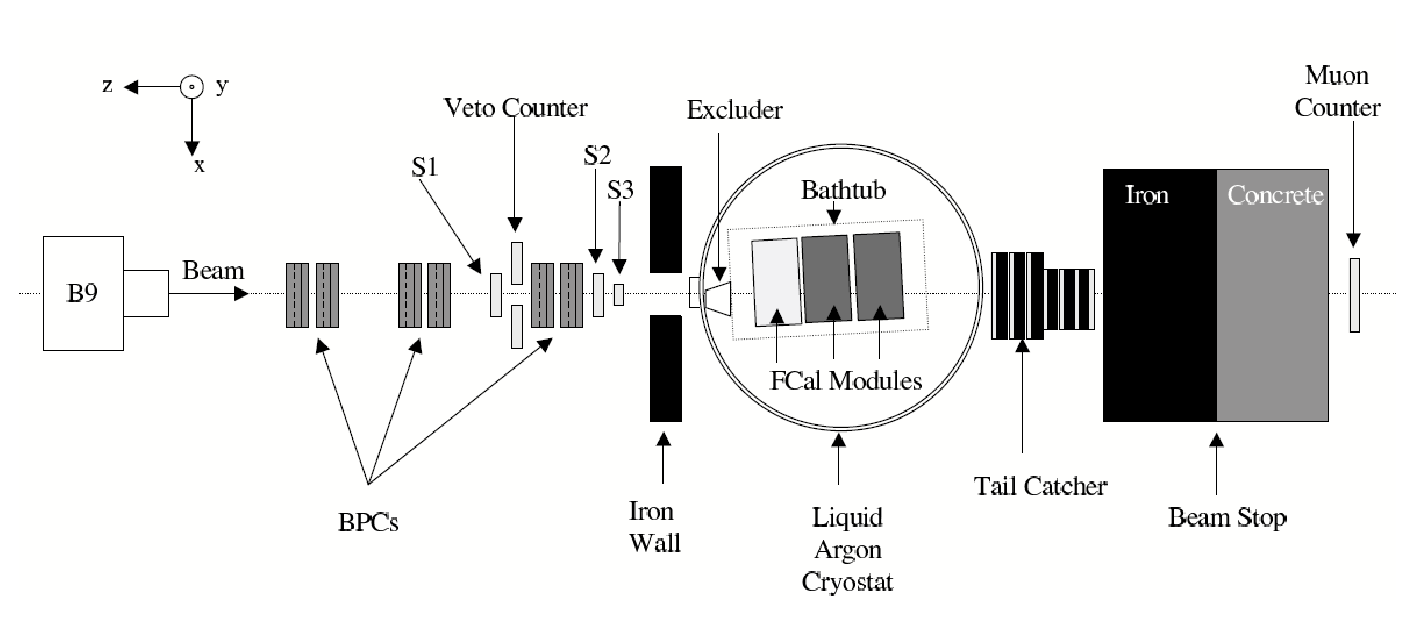
\includegraphics[width=0.8\linewidth,angle=0]{TB_Beamline}
\end{center}
%\centerline{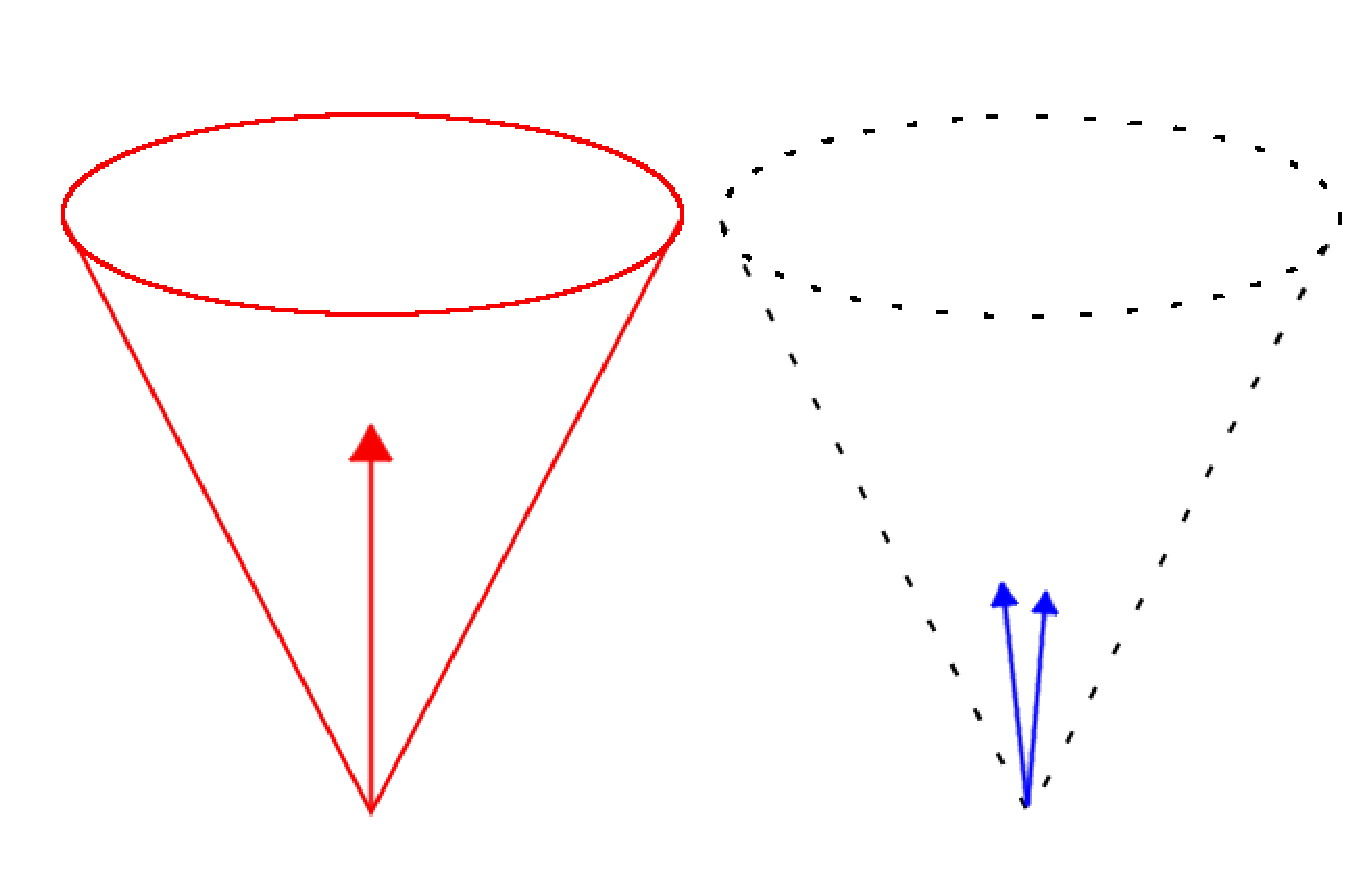
\epsfig{file=./figs/collinear.eps  , width=0.95\textwidth}}
\caption[Beamline setup for the 2003 beam test]{Diagram showing the setup used for the 2003 FCal beam test (not to scale).}
\label{fig_TB_beamline}
\end{figure}

\begin{figure}[tb]
\begin{center}
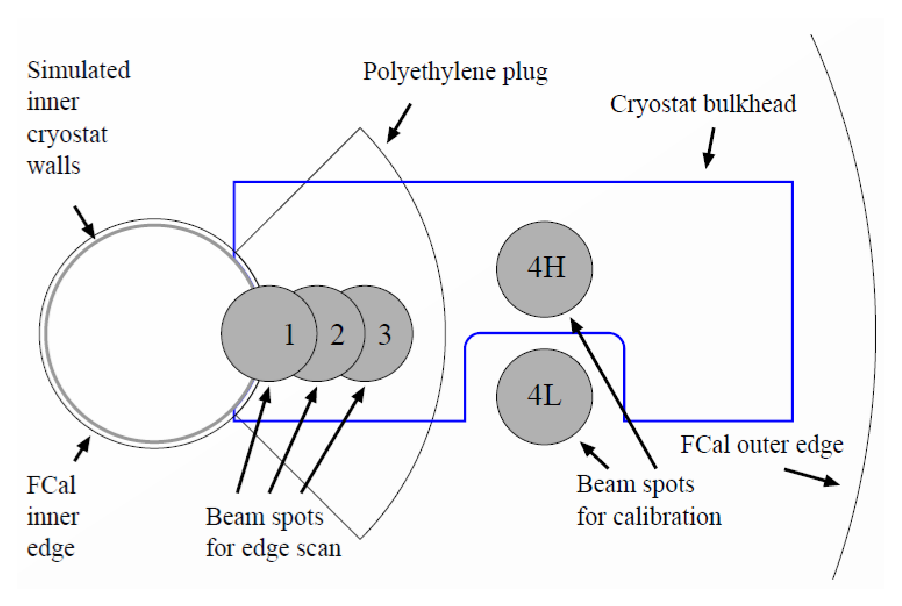
\includegraphics[width=0.8\linewidth,angle=0]{TB_beamspots}
\end{center}
%\centerline{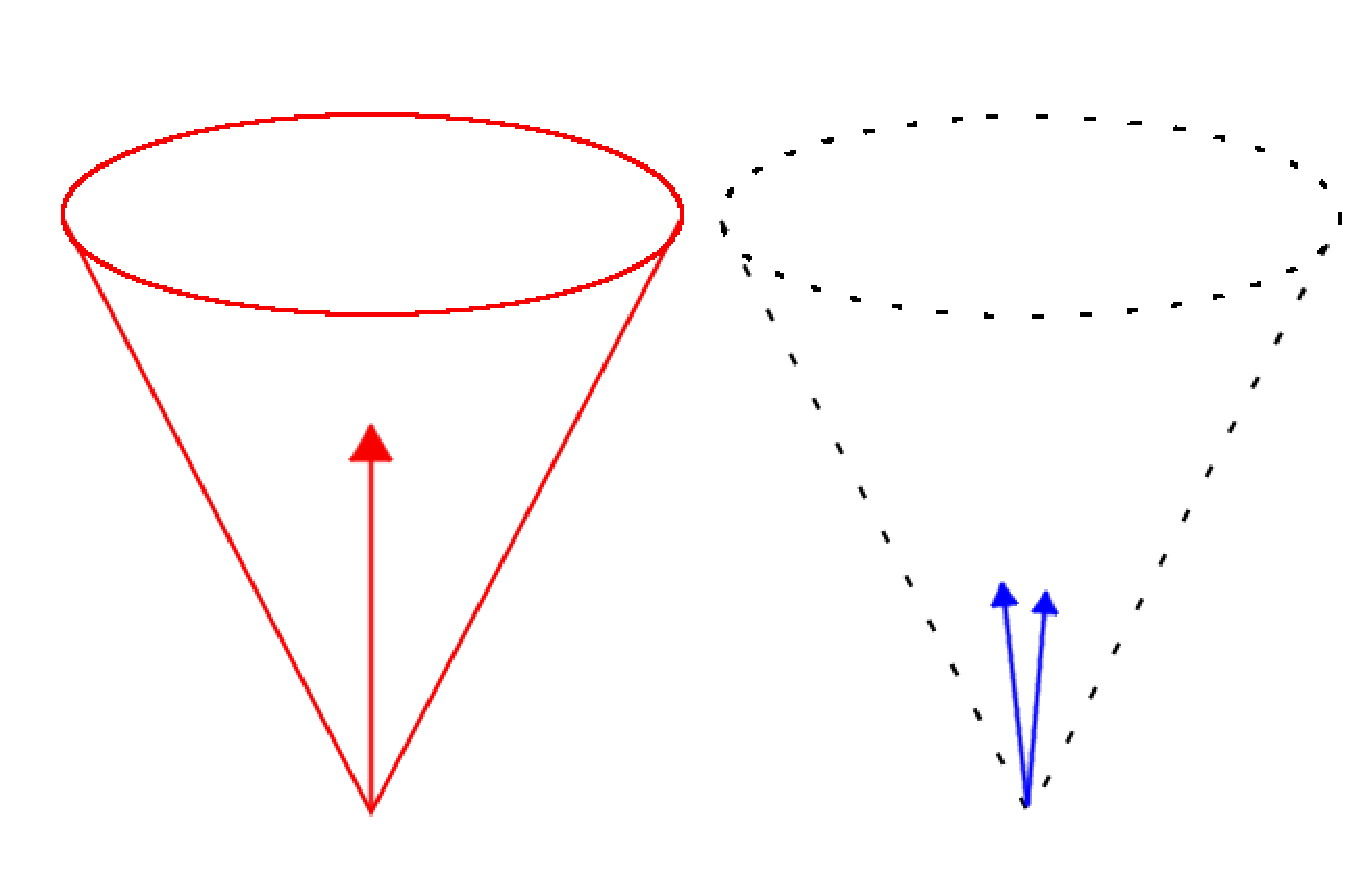
\epsfig{file=./figs/collinear.eps  , width=0.95\textwidth}}
\caption[Beamspots studied in the testbeam]{Beamspots studied in the testbeam.}
\label{fig_TB_beamspots}
\end{figure}

A diagram of the beamline is shown in Figure~\ref{fig_TB_beamline}. Beam particles emerge from the B9 magnet, travelling a distance of 32 metres and passing through several sets of instruments before reaching the FCal. The B9 magnet was used to control the vertical inclination of the beam, and thus the vertical position of the beamspot on the FCal face\cmt{ could be controlled via manipulation of the currents in the B9 magnet}. The cryostat containing the FCal was able to be translated horizontally and rotated slightly, providing control over the horizontal position of the beamspot and the angle at which the beam particles struck the front face of the calorimeter. A total of 5 beamspots were used, labelled 1,2,3, 4L and 4H, as illustrated in Figure~\ref{fig_TB_beamspots}. Positions 1,2 and 3 were used to study the effects of energy leakage down the beampipe from particles impacting close to the inner edge of the detector. High energy ($\sim$200 GeV) beams of electrons and pions were used to provide data at these positions, and the results of these studies can be found in \cite{LouiseThesis,TB03_tbp}. Position 4L was used to study the intrinsic response of the FCal with a minimal amount of material between the calorimeter and the incoming particles, whereas position 4H was used to simulate a more \atlas-like environment with additional dead (i.e. uninstrumented) material introduced into the beamline. Electrons and pions at energies from 10-200~GeV were used at these beamspots. This chapter will discuss the analysis of data taken at positions 4L and 4H, and the comparison of these results to those obtained from Monte Carlo simulations carried out using the \atlas software framework, \athena, and \geant, which simulates the interactions of the beam particles with the calorimeter.
 



\section{Beamline Instrumentation}
%beam instrumentation and upstream material 
\label{sec_TBoverview_beamline}
\cmt{bpcs: positioning or profile? positioning in FCal paper}
Eight beam positioning chambers (BPCs) were used to provide tracking information on beam particles.
Four of these BPCs were of a more sophisticated design, one pair of which was located about 1.6 metres downstream of the B9 magnet while the other pair was situated 3 metres upstream of the FCal, on an adjustable table described below. These chambers each contain two readout planes, oriented at right angles such that measurements of both transverse coordinates may be made. Each readout plane covered an area of 120mm~$\times$~120mm, and had an average resolution of around 130~$\mu$m. The other four BPCs were of an older design and were able to measure a single track coordinate with a resolution of about 325~$\mu$m. These were positioned in the middle of the beamline (about 20m from the FCal), with two BPCs measuring the $x$ coordinate of the beam particles and the other two the $y$ coordinate. In total, the eight BPCs provide six independent measurements of the $x$ and $y$ coordinates of the beam particle tracks.

%\red{should talk about alignment here, or in results}
A mapping between BPC and calorimeter coordinate systems was established through analysis of electron data~\cite{Fcalpaper}. The track measured by the BPCs was projected on to the calorimeter in order to obtain the beam impact point in the BPC coordinate system. This was then associated with the barycentre of the energy deposited in FCal1 using the calorimeter coordinate system. However, the finite granularity of the calorimeter readout tended to bias the position of the energy barycentres towards the centre of the readout cells. This mapping was improved by considering the ratio $E_\mathrm{max}/E_1$, where $E_1$ was the total energy deposited in FCal1 and $E_\mathrm{max}$ was the largest energy value contained in a single channel. This ratio was plotted as a function of (BPC) $x$ and $y$, with minimal values in the ratio corresponding to cases where energy was shared evenly between multiple channels. The positions of the minima could thus be associated with cell boundaries in the calorimeter coordinate system, which then allowed the mapping between BPC and calorimeter coordinate systems to be determined with greater precision. The uncertainty associated with this mapping is $\pm0.12$ mm in the $x$ coordinate and $\pm 0.25$mm in the $y$ coordinate~\cite{LouiseThesis}.
%
%
%Emax - max channel energy
%E1 - total FCal1 energy
%scan across cell boundaries. 





The adjustable table was positioned about 2 metres upstream from the cryostat, on which three scintillators (S1, S2, S3) were positioned. These scintillators were polystyrene-based, and were used for triggering and ``beam cleaning'', which is discussed in Section~\ref{sec_event_selection}. All three scintillators were 1 cm thick, with S1 and S2 having cross-sectional dimensions of 10cm $\times$ 10cm, while S3 had dimensions 7cm $\times$ 7cm. A veto counter was also present on the table, consisting of rectangular piece of scintillator (63cm $\times$ 63cm $\times$ 5cm) with a circular hole 65mm in diameter that the beam passed through. The height of the table could be varied such that the beam instruments were in the appropriate position for the beamspot under study. 

As the liquid argon gaps in the FCal are much smaller than those used in typical liquid argon calorimeters, FCal channels are susceptible to shorts should any conductive debris find its way into the liquid argon. Because it was particularly difficult to clean the interior of the cryostat, the FCal was housed inside a ``bathtub'' which sat inside the cryostat. This was made from stainless steel 1.5 mm thick, and had a rectangular shape. Holes were present on its sides to allow the liquid argon to flow in as the cryostat was filled, but these were covered with a fine mesh to keep any debris out. 

\begin{figure}[tb]
\begin{center}
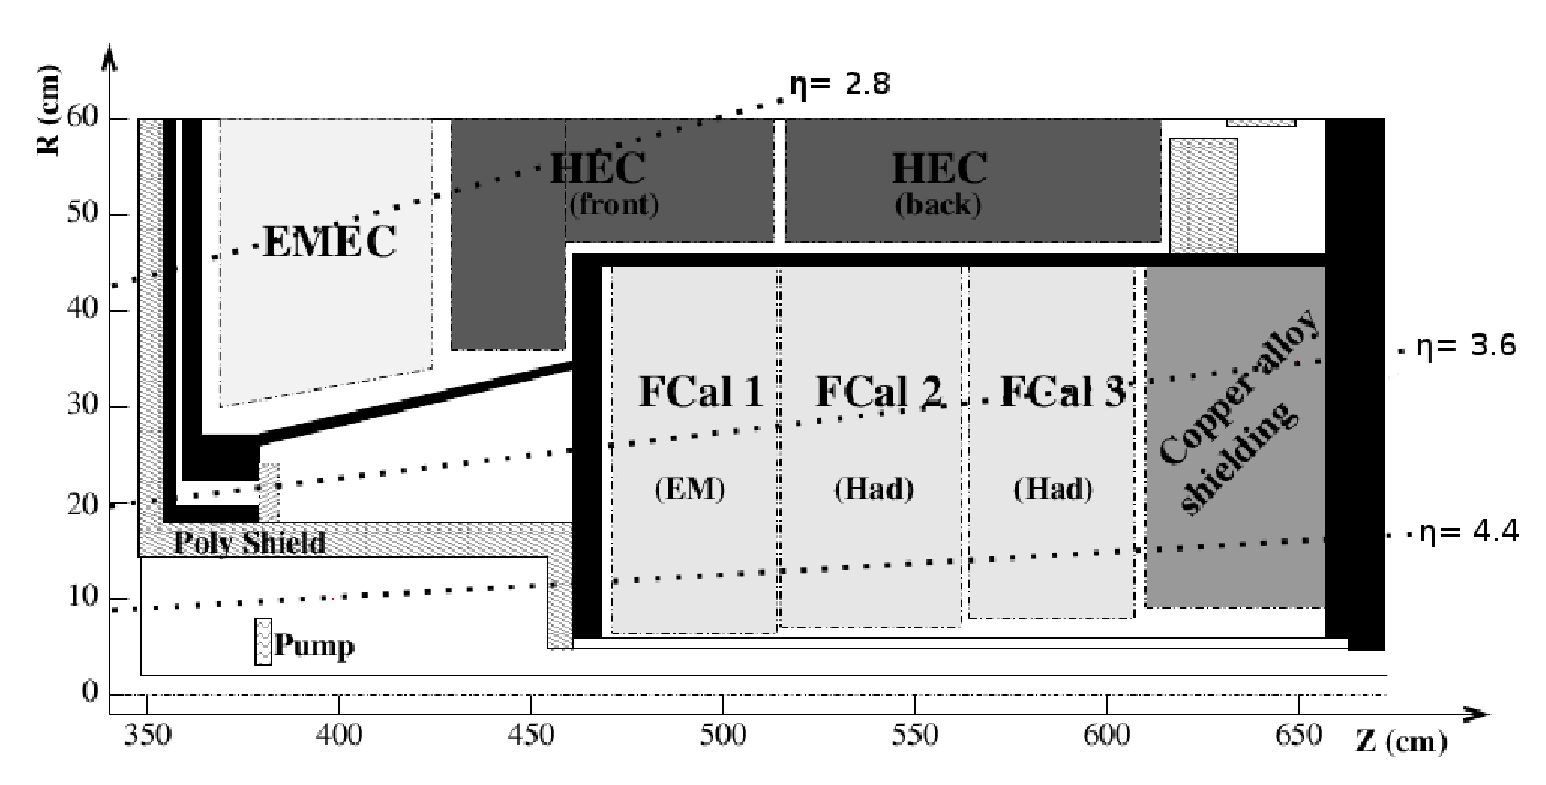
\includegraphics[width=0.8\linewidth,angle=0]{atlas_EC_xsec2.eps}
\end{center}

\caption[End-cap cross-section]{Cross-section of FCal positioned within the end-cap cryostat, showing the inactive material present in this region. The material in black is associated with the end-cap cryostat.}
\label{end_cap_xsec_2}
\end{figure}

In order to simulate a more \atlas-like environment for data taken at positions 1,2,3 and 4H, additional material was inserted into the beamline. A cross-section of part of the \atlas end-cap is shown in Figure~\ref{end_cap_xsec_2}, showing the uninstrumented (or ``dead'') material present in this region. An aluminium plate 50.8 mm thick was bolted to the inside of the bathtub to model the cryostat bulkhead (i.e. the cryostat material located just in front of FCal1 in Figure~\ref{end_cap_xsec_2}), with a slot cut out of the plate such that the material would not affect beams at position 4L. The area covered by this plate is labelled as ``Cryostat bulkhead'' in Figure~\ref{fig_TB_beamspots}.

The \atlas JM shielding~\cite{detector_paper} (labelled ``Poly Shield'' in Figure~\ref{end_cap_xsec_2}) is made of boronated polyethylene and is present in \atlas to prevent albedo radiation from scattering back into the inner detector. This was modelled in the beam test by placing a wedge shaped piece of polyethylene on the outside of the bathtub such that it covered positions 1, 2, and 3, simulating the toroidal ``plug'' part of the shielding that lies close to the beam pipe and adjacent to the cryostat bulkhead. Figure~\ref{tub_photo} shows a photograph of the bathtub with this polyethylene attached to its exterior wall. An iron wall was located between the adjustable table and the cryostat. This wall had a 10cm x 10cm slot cut into it to allow the beam to pass through. When taking data at position 4H, a rectangular piece of polyethylene with dimensions 5~cm~$\times$~20~cm~$\times$~1~m was placed at an angle in this slot. This was done in order to model the tube shaped part of the JM shielding that runs parallel to the beam axis. When running at position 1, a small piece of aluminium was instead placed in this slot, simulating the ion pump present close to the beampipe in \atlas (labelled ``Pump'' in Figure~\ref{end_cap_xsec_2}).

\begin{figure}[tbp]
\begin{center}
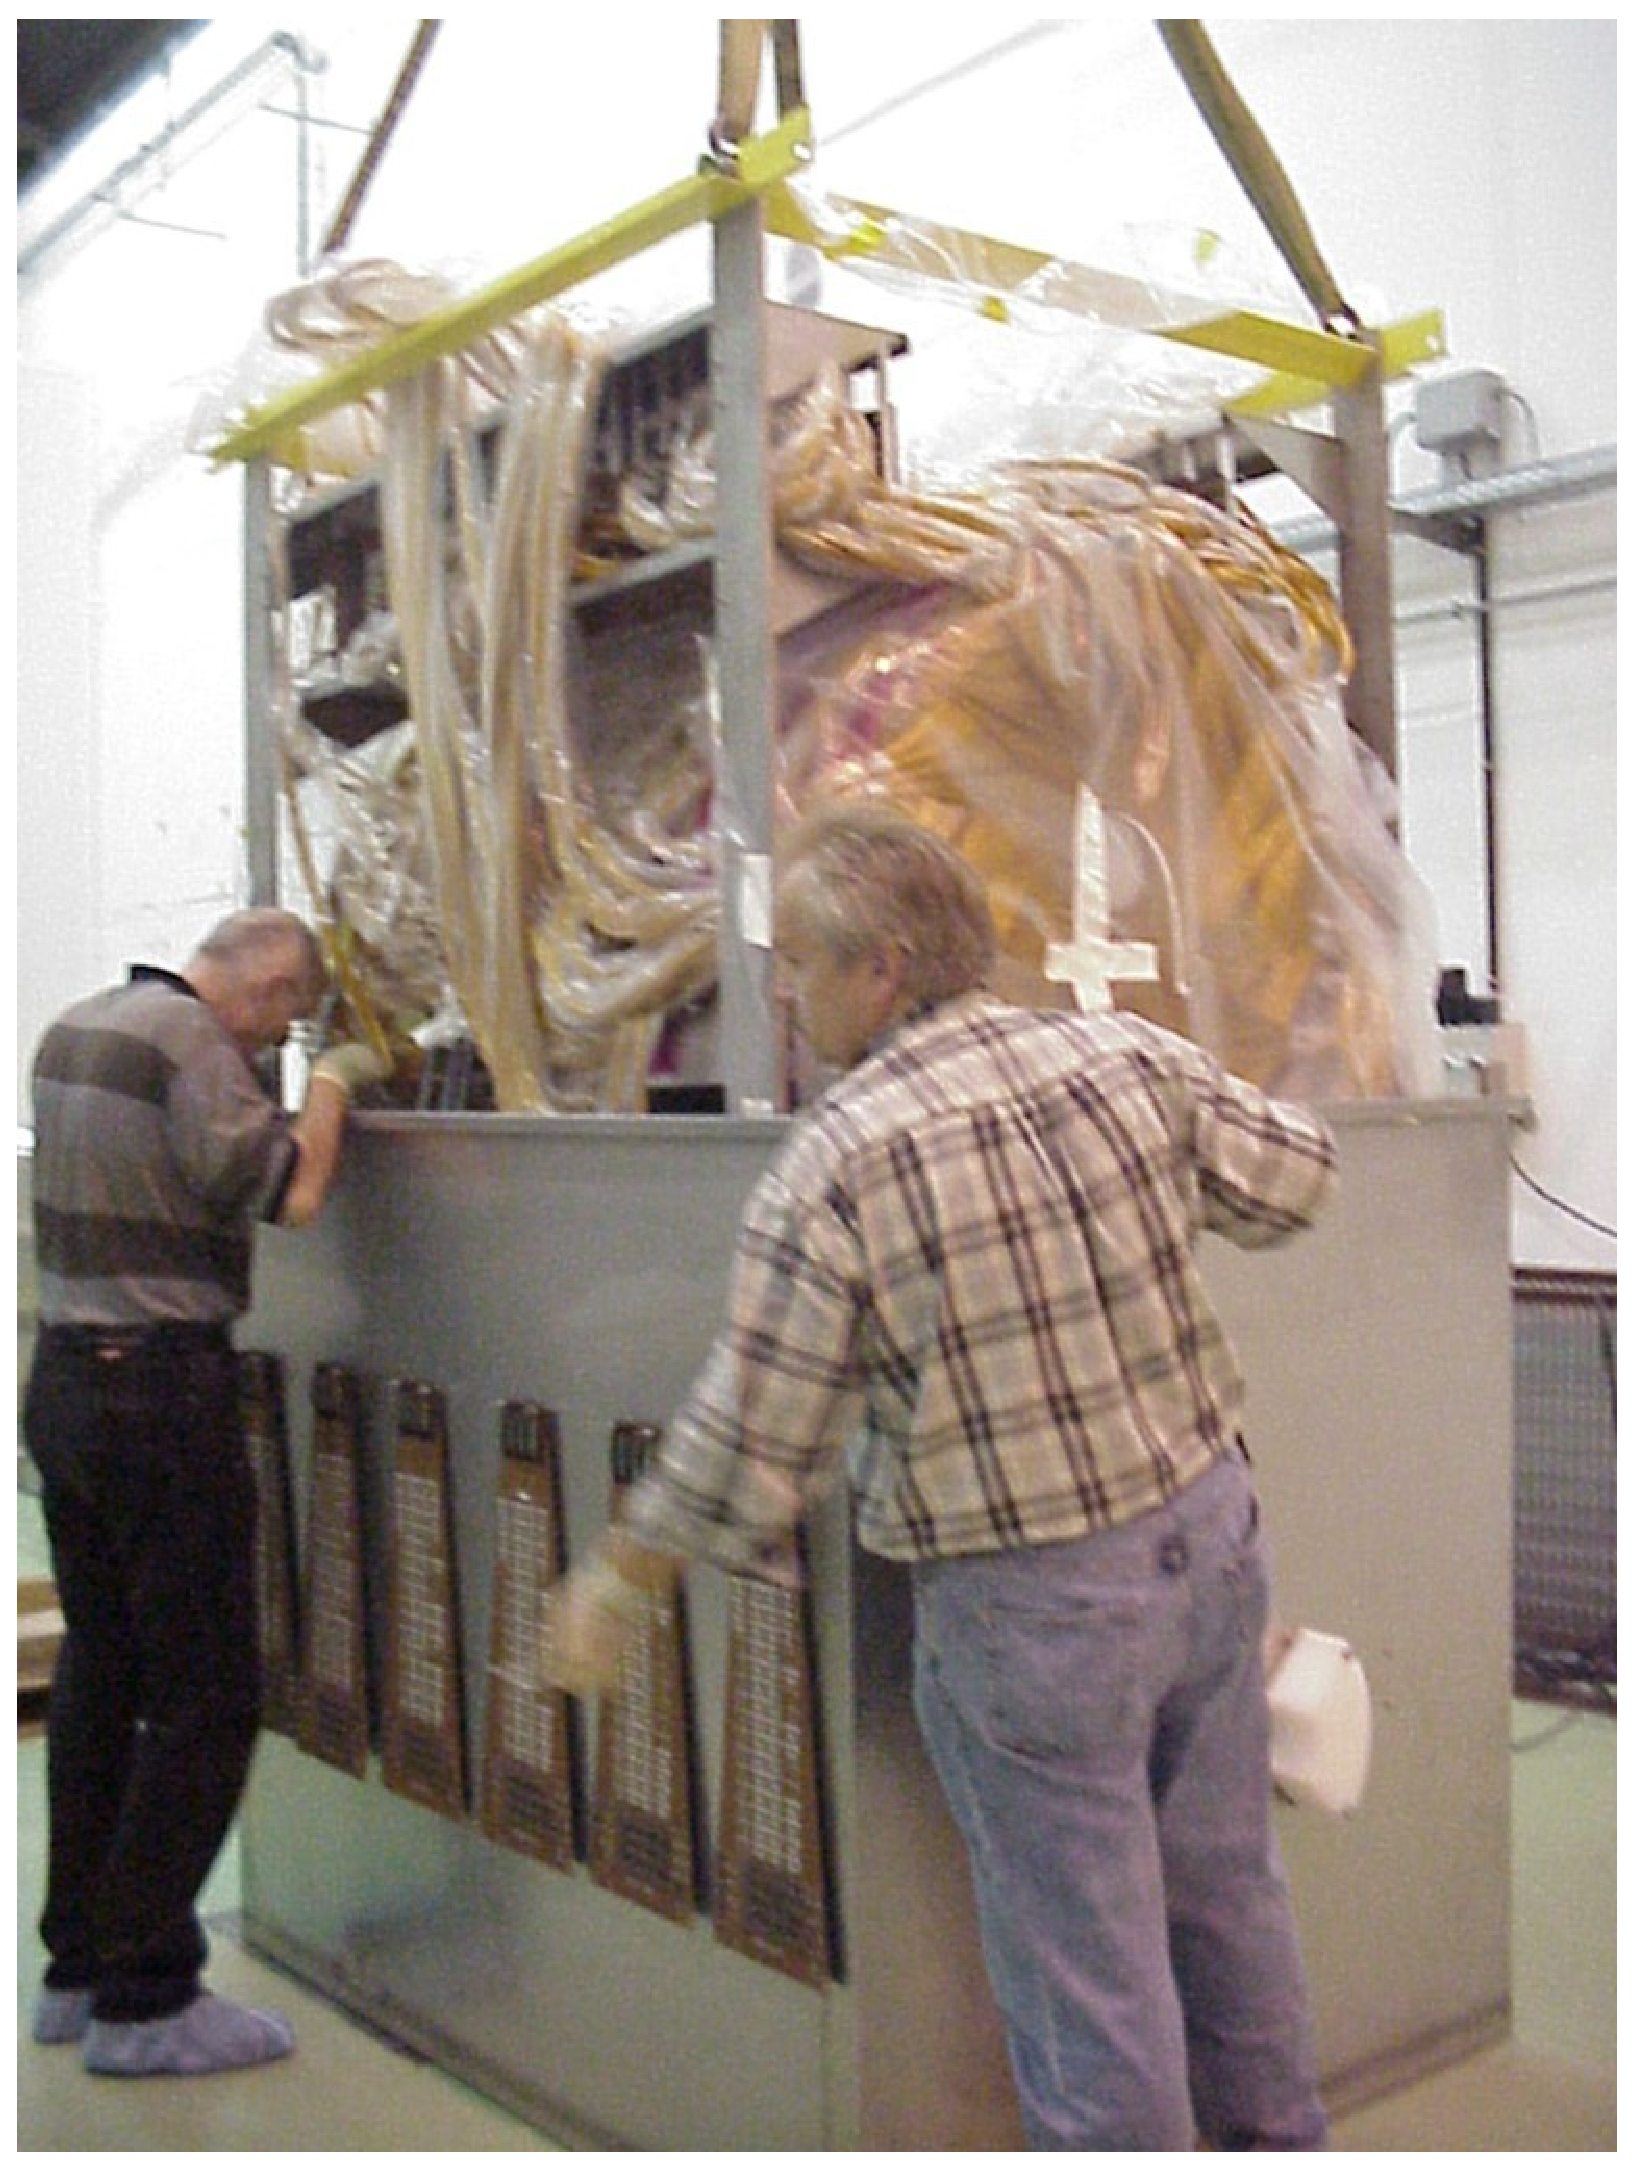
\includegraphics[width=0.5\linewidth,angle=0]{tub_photo.eps}
\end{center}
\caption[Photograph of the FCal and bathtub prior to beam test]{Photograph of the  FCal being lowered into the bathtub used for the beam test. The polyethylene used to simulate the plug portion of the ATLAS JM shielding is visible on the front of the bathtub, while the summing boards can be seen on the left side.}
\label{tub_photo}
\end{figure}




%An ``excluder'' made of RohaCell was also attached to the outside of the bathtub.
In \atlas, the area within the cone-shaped part of the FCal support tube (just in front of the FCal, as shown in Figures~\ref{end_cap_xsec_2} and \ref{fig_cut}) is evacuated. The support tube used in \atlas was not present during the testbeam, and the FCal modules were instead mounted on a purpose-built stand within the cryostat. An ``excluder'' made of RohaCell was attached to the outside of the bathtub, in order to prevent the region of space corresponding to the evacuated region in \atlas from being filled with liquid argon. 
% In \atlas the area between the FCal support tube and the beampipe is evacuated, and so the excluder was placed inside the cryostat to prevent this space from being occupied by liquid argon.
 The density of RohaCell is 0.011 $\mathrm{g}/\mathrm{cm}^3$ whereas that of liquid argon is 1.43 $\mathrm{g}/\mathrm{cm}^3$, so the RohaCell provides a relatively good approximation of a vacuum. A hollow stainless steel cylinder was also placed inside the FCal during the beam test to simulate the beampipe, and also to exclude liquid argon from this region.
 
Note that in \atlas, there is additional material upstream of the FCal that has not been considered here. The additional material described above was intended to model only the upstream material associated with the end-cap cryostat and the JM shielding. At the time of the beam test, the amount of material associated with the inner detector and its services was not well known, and so no attempt was made to simulate it. However, in \atlas, particles reaching the FCal will first have to pass through this material.

A tail-catcher calorimeter comprised of layers of steel and scintillator was positioned downstream of the cryostat. Behind this was a beamstop of iron and concrete, and beyond that a muon counter was located. The tail-catcher and muon counter were only used for muon identification: energy deposited in the tail catcher was not considered when measuring the response of the FCal, or in the derivation of any weights used for hadronic reconstruction in the analysis presented here.

A CEDAR (Cherenkov Differential counter with Achromatic Ring focus, \cite{CEDAR_note}) detector was located upstream of the B9 magnet and used for particle identification. The CEDAR detector consists of a chamber filled with gas (He) at high pressure. As beam particles pass through this chamber, they  emit Cherenkov radiation at an angle that depends on their velocity and mass. The optics of the CEDAR  collect this light and focus it into a ring-shaped image, with different types of particles giving rings of different radii. An adjustable annular aperture is positioned in front of a series of photomultipliers, such that these detect light only from rings of a given radius. The radius selected by the aperture may be tuned such that signal from the photomultipliers corresponds to a beam particle of the desired mass.

% As beam particles passed through a series of chambers filled with gas (He or $\mathrm{N}_2$) at high pressure, and emit Cherenkov radiation at an angle that is dependant on their velocity and mass. The optics of the detector then focus this into a ring, with different types of particles producing rings of differing radii. 

%
%
%
%
%
%
%
%
%\begin{figure}[tb]
%\begin{center}
%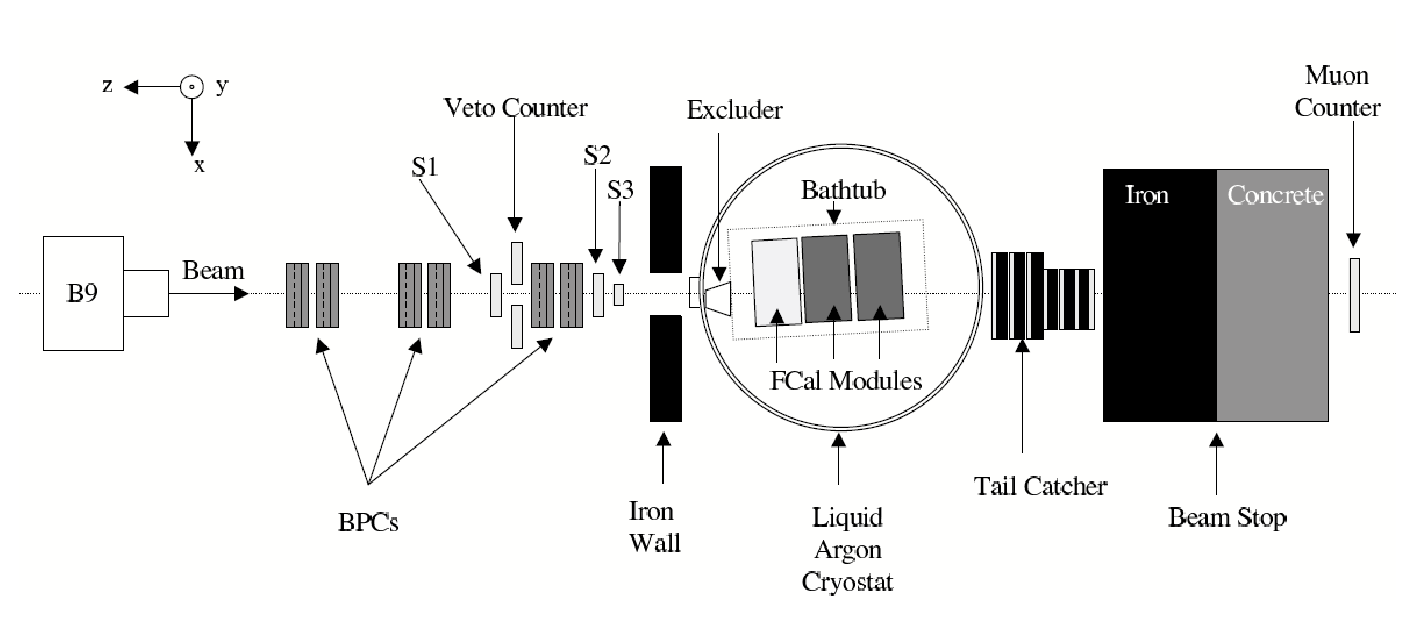
\includegraphics[width=0.8\linewidth,angle=0]{TB_Beamline}
%\end{center}
%%\centerline{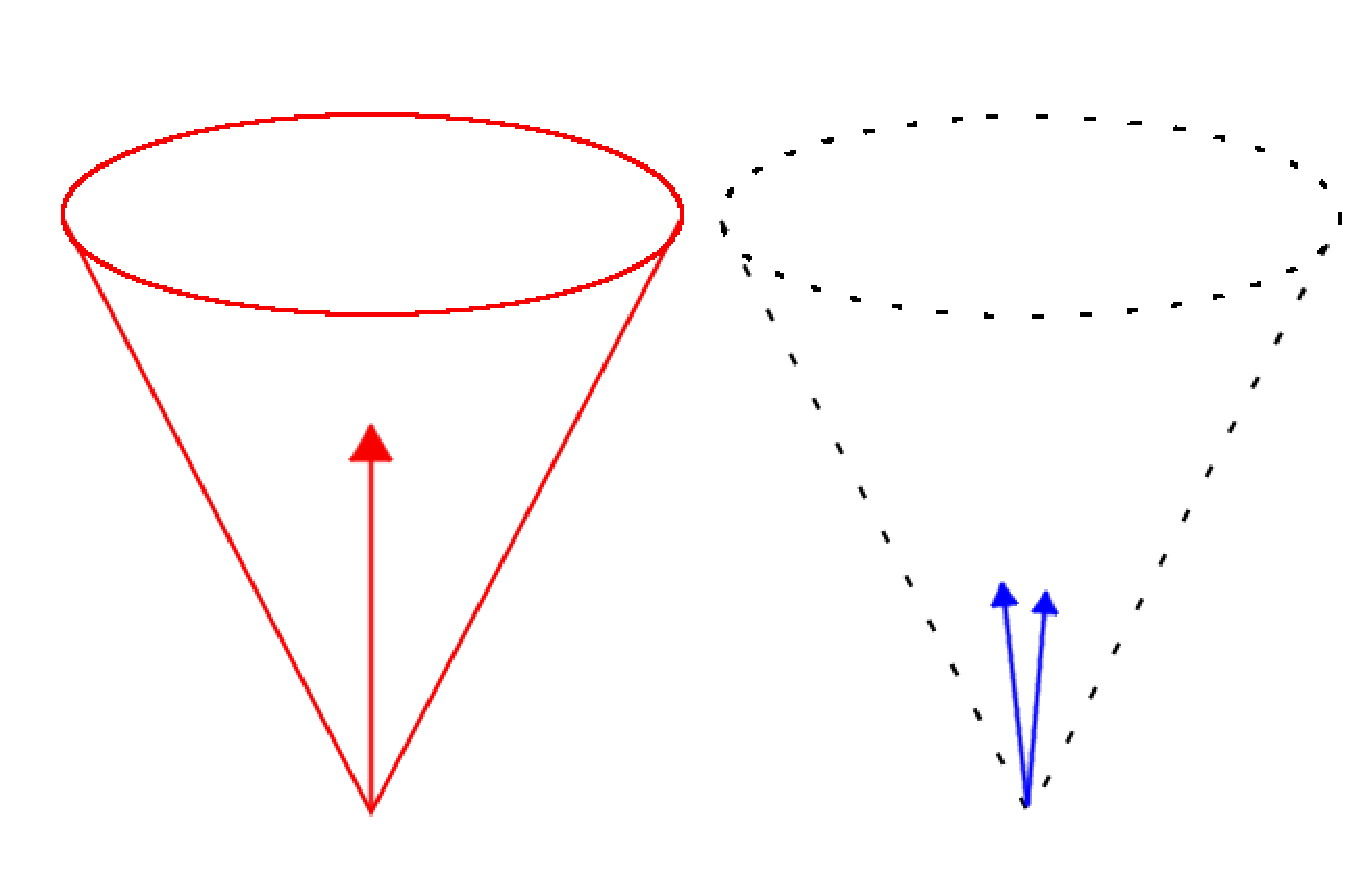
\epsfig{file=./figs/collinear.eps  , width=0.95\textwidth}}
%\caption{Diagram showing the setup used for the 2003 FCal beam test (not to scale).}
%\label{fig_TB_beamline}
%\end{figure}
%
%\begin{figure}[tb]
%\begin{center}
%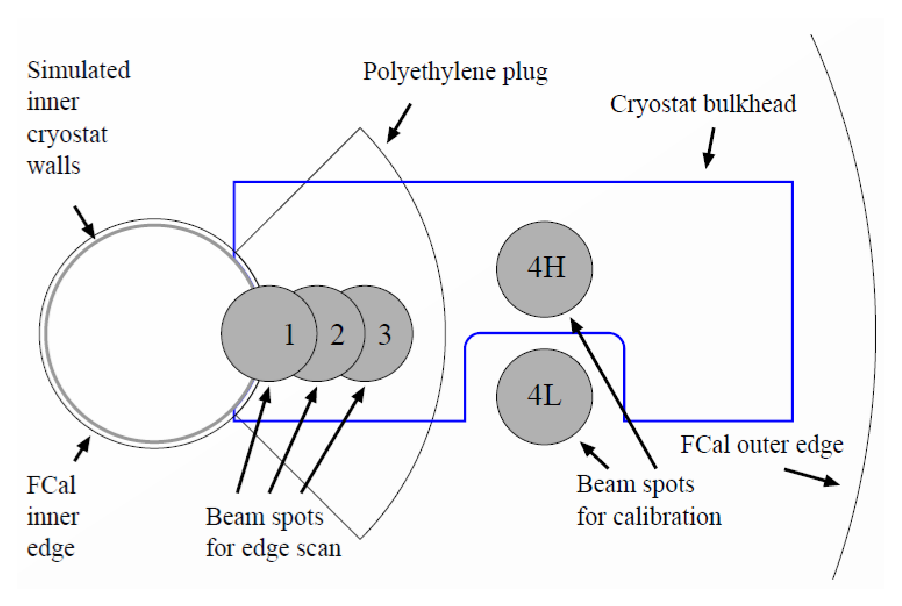
\includegraphics[width=0.8\linewidth,angle=0]{TB_beamspots}
%\end{center}
%%\centerline{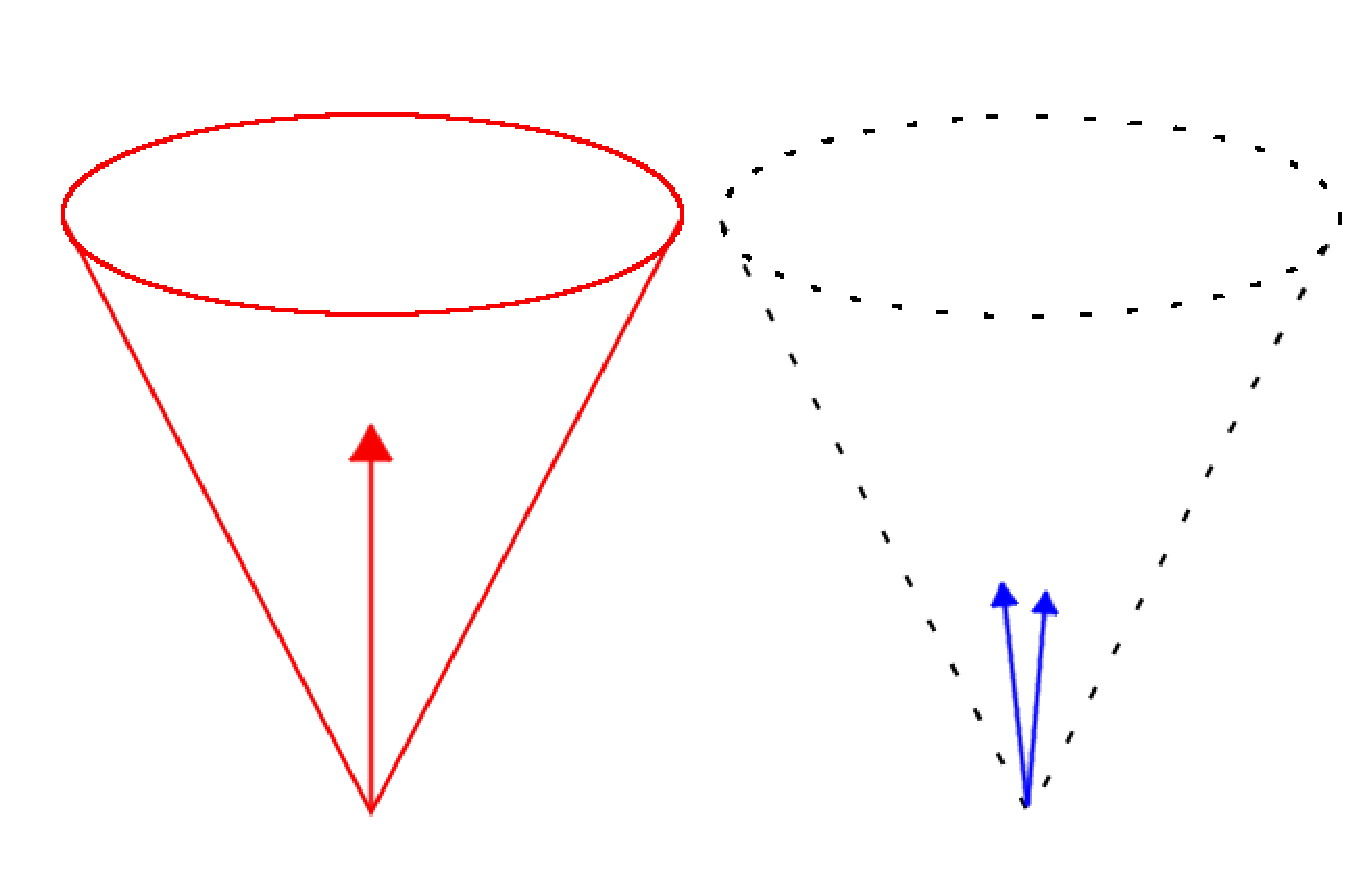
\epsfig{file=./figs/collinear.eps  , width=0.95\textwidth}}
%\caption{Beamspots studied in the testbeam.}
%\label{fig_TB_beamspots}
%\end{figure}
%
%


%
% 
%
% 
%
% Protons from the SPS beam were directed onto targets of in order to produce a secondary/tertiary beam of the desired particle type.\red{(which targets for which particles?)} . \red{Then a magnet (velocity selector) was used to select particles of the desired type and energy}. 
%maybe skip the details here. secondary/tertiary beam emerges from B9, then stuff happens.
%
%
%
%
%This secondary beam of particles then passed through a bending magnet ("B9"), which controlled the vertical inclination of the beam. The vertical position of the beamspot on the FCal face could thus be manipulated by varying the currents in the B9 magnet. 
%
%
%The cryostat containing the FCal was positioned 32 metres away from the B9 magnet. The 
%
%
%
%Six Beam Profile Chambers (BPCs) are used to obtain information on the trajectory of the beam particles. The 
%
%BPCs
%
%table scintillators, veto counter
%
%Iron wall, upstream material
%
%Cryostat
%aluminium plate, excluder
%bathtub
%FCal
%
%Tail Catcher
%
%
%\red{move FCal electronics and LAr signal reconstruction to Detector chapter. Keep Timing and offline reconstruction here.}



\subsection{Timing and Pulse Shapes}
\label{sec_TBoverview_timing}
%done using ofc method described in Section~\ref{sec_signal_rec_OFC}.\cmt{\red{Test beam studies pulse shapes\ldots}} 
Reconstruction of the calorimeter signals was carried out using the OFC method described in Section~\ref{sec_signal_rec_OFC}.\cmt{ A SPICE \cite{SPICE_paper} simulation of the electronics chain was used to obtain an initial estimate of the pulse shape used in the OFC calculation. This estimate was then improved using an iterative procedure that incorporated data taken during the beam test. The data used in this procedure was taken from events in which the signal pulses had large amplitudes, in order to ensure that the signal was coming from a physical energy deposit.}
Pulse shapes were sampled in time with the TTC clock on the FEBs (described in Section~\ref{sec_FCal_electronics}). Seven samples were recorded for each pulse during physics runs, with the timing adjusted such that, on average, the fourth sample was coincident with the pulse peak. The first sample could thus be used to monitor noise, as it was recorded before the signal pulse started to rise. In \atlas the TTC system is synchronised to the LHC clock, such that samples are taken in time with each bunch crossing. This was not the case during the beam test, as beam particles arrived at random times with respect to the TTC clock. Timing for the event was taken from the S1 scintillator. A LeCroy 2228A Time to Digital Converter (TDC)  with a timing resolution of 50 ps was used to measure the phase difference between the event trigger and the TTC clock, with the trigger from the S1 scintillator used as a start signal and the clock pulse from the TTC system used as a stop signal. The TDC only measured a phase difference between the start and stop signals, and so readings close to 0 or 25 ns were ambiguous. To resolve this a second TDC was used in which the stop signal was delayed by 10 ns, which allowed the time interval between the beam trigger and the TTC pulse to be determined uniquely. 

While the OFC method is capable of handling time differences between pulse peaks and sample times, the Taylor expansion used in equation \ref{eq_OFC_taylor} becomes invalid when this time, $\tau$, becomes large. To avoid this issue, events are binned according to the phase time measured by the TDC, using 25 bins of width 1 ns. A set of OFCs is calculated for each bin using a pulse shape that has been shifted in time by the relevant amount. During event reconstruction, the amplitude of each pulse is obtained by using the set of OFCs corresponding to the TDC phase time for that event. Only a single set of OFCs is required at \atlas, as in this case the TTC clocks are synchronised with that of the LHC, and so the samples are recorded in time with the LHC clock.

%
%For each of the 25 bins, a set of OFCs are calculated using a pulse shape shifted in time by the relevant amount. During signal reconstruction, the TDC phase time is used to look up the correct set
%
%
%
% 
%
%A SPICE simulation of the electronics chain is used to obtain an initial estimate of the pulse shape used in the OFC calculation. This estimate was then improved using an iterative procedure that incorporated data taken from physics runs. 
%
%To avoid this issue, 
%
%%The pulse shapes used in deriving the OFCs are taken from physics data, using events which had a large peak and were thus due to physical energy deposits.
%A SPICE simulation of the electronics chain is used to obtain an initial estimate of the pulse shape used in the OFC calculation. This estimate was then improved using an iterative procedure that incorporated data taken from physics runs.   
%
%
%The samples were fitted to a pulse shape prediction obtained through simulation of the electronics chain in order to find the time and amplitude of the pulse peak. Each pulse was then shifted and scaled so that the peak occurred at time zero and had unit height. 
%
%
%
%
%
%
%OFC calculation.
%
%
%
%
%
% TTC every 25 ns.
%S1 random with respect to this, so LeCroy TDC used to measure time shift/phase between TTC and S1 with 50ps resolution. Second TDC used to remove phase ambiguity at 0/25 ns (are things exactly in time or 25ns off?) 
%
%because things arrive asynchronously, OFCs computed for 1ns bins of phase difference, i.e. 25 different sets of OFCs derived. timing phase used to select OFCs used for signal reconstruction.
%
%Pedestal - physics triggers, first (of seven) sample used for pedestal studies. Pedestal subtracted from pulse. 
%
%Pedestal value calculated for each channel, run by run. Noise for each sample taken as RMS of pedestal - 3.2 ADC on average.
%
%random trigger data used for noise autocorrelation?
%
%
%
%
%
%
%
%
%
%
%

\subsection{Offline Reconstruction}
\label{TBoverview_offline}
Offline reconstruction of the beam test data is carried out using \athena. A flowchart depicting the data structures and algorithms used in the reconstruction of data and simulation events is shown in Figure~\ref{TB_data_flowchart}. For each event, the LArRawChannelBuilder algorithm retrieves the pulse samples (which are stored as LArDigits), and fetches the appropriate set of OFCs from a database. The pedestal is then subtracted from these samples and the OFCs are applied, giving the amplitude of the pulse in ADC counts. This amplitude is then converted to an energy using a factor (the ADC2MeV value discussed in Section~\ref{ECal}) that depends on the channel and gain. The energy of the channel, in MeV, is then stored as a LArRawChannel object. Another algorithm is then used to create a CaloCell object from this LArRawChannel. From the CaloCell, the position, time, energy, quality, and four-momentum of the channel may be retrieved, making CaloCells suitable objects for use in data analysis. Because of this, CaloCell information is recorded by default in Event Summary Data (ESD) files, one of the standard file formats used by \atlas. CaloCells are also used as input during the formation of topological clusters (discussed in Section~\ref{FCALTB_topoclusters}), which in turn are used as input for jet-finding and missing-energy algorithms.

For initial studies of the testbeam data, the ADC2MeV factors used in the reconstruction were set to 1, so that the final energies were obtained in terms of ADC counts. This was done so that the actual ADC2MeV values could be extracted from the data more easily. However, the LArRawChannel class used in \athena stores channel energies as an integer number of MeV, as energies less than 1 MeV are deemed insignificant. An unforeseen consequence of this was that in earlier versions of the testbeam analysis, cell energies were truncated (rounded down) to an integer number of ADC counts. This rounding meant that energy was effectively lost during the reconstruction process, up to $\sim$80 MeV per cell in FCal1 and $\sim$160 ($\sim$185) MeV in FCal2 (FCal3). This had a small effect on the electron results, but a more significant effect on the hadron results due to the broader showers and higher ADC2MeV factors associated with the hadronic modules. The bug has since been fixed, and none of the results presented here are affected by it. The effect that this bug had on the previously published results \cite{Fcalpaper} was small, and will be discussed further later in this chapter.


\begin{figure}[tb]
\begin{center}
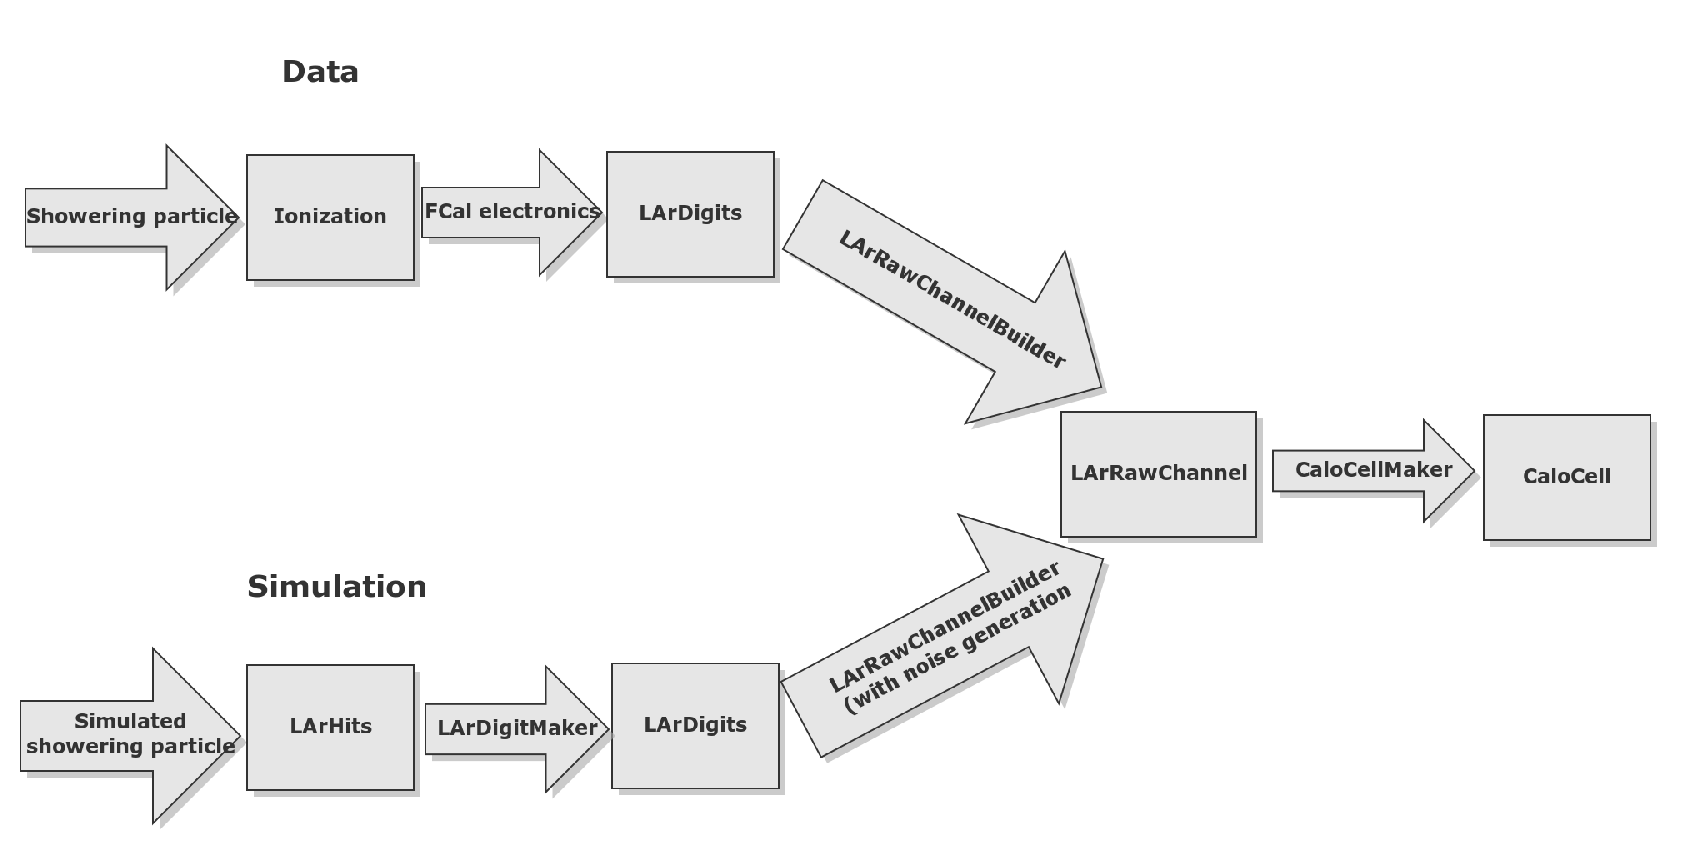
\includegraphics[width=0.9\linewidth,angle=0]{TBoverview/TB_flowchart2.eps}
\end{center}

\caption[Flowchart showing the algorithms used during reconstruction]{Flowchart showing the processes/algorithms and data structures involved in the reconstruction of testbeam data and simulation results.}
\label{TB_data_flowchart}
\end{figure}
%\clearpage
\section{Monte Carlo Simulation}
%\subsection{Monte Carlo}
%\subsection{reconstruction}
%\subsection{noise}
%Athena/G4/geometry
%digi/reco
%noise


A Monte Carlo simulation of the testbeam setup has been developed within the \athena framework. \cmt{The simulation describes all elements of the beamline from the B9 magnet to the tailcatcher.} {\tt G\scalebox{0.9}{EANT4.9.2}} \cite{geant4} is used to simulate interactions of the beam particles with beamline elements and the calorimeter. The results of this simulation are then reconstructed and analysed in the same manner as the data. The forward calorimeter beam test provides a clean environment in which the results from data may be compared to those obtained from simulations. As all of the hadronic calibration schemes used at \atlas are derived from Monte Carlo, it is important to understand the how well these simulations agree with data.

\subsection{GEANT4 Simulation of the Forward Calorimeter Beam Test}
\label{TB_overview_g4}
Geometry in \geant is described in terms of volumes. A ``solid volume'' is first created to describe the shape of a given object. This is then used to derive a logical volume, which inherits the shape of the solid and is associated with a material. A material type is defined by specifying the relative mass fractions \cmt{of the elements of which it is composed} of its constituent elements and the density of the material. Logical volumes are then used to construct physical volumes, which inherit the shape and material information from the logical volume. A physical volume also has a position and orientation assigned to it, and it is by positioning these physical volumes that the geometry of the simulation is defined. A special physical volume, the world volume, is created first. All subsequent physical volumes are then placed either inside the world, or inside another physical volume. 
%The position and orientation of a physical volume are specified through transformations: rotations and translations. A physical volume is placed at the origin of the volume it is inserted into, and transformation operations are then applied to reposition it. 

The description of the beamline used in the simulation contains all beamline elements downstream of the B9 magnet, including all scintillators, BPCs, cryostat material, beampipes, the tailcatcher and the muon counter. Most of these objects are defined from scratch, however the description of the FCal is taken from that used in the full \atlas simulation (although this is modified slightly as discussed below), while the H6 cryostat description has been taken from another testbeam simulation. Elements upstream of the B9 magnet, such as the CEDAR detector, have not been included. The scintillators and BPCs that are included in the simulation are only treated as dead material, no (simulated) signals are obtained from them.

%The description of the FCal has been modified in some respects,
Small modifications to the FCal definition used in the simulation were made in order to improve some aspects of the material description. In the default definition of the FCal, WFeNi is the material used for the rods in the hadronic modules, whereas they are actually made of pure tungsten which has a slightly higher density. 
%The density of the absorber matrix was also corrected, as an updated estimate of this value was obtained. 
The correct materials and densities (given in Section~\ref{chap_Detector_FCal}) have been used in the testbeam simulation.

%The abstract way in which positions are defined can also lead to errors. \geant uses matrices to represent transformations, and so the order of operations are important. When a physical volume is inserted into the world (or another physical volume), it is placed at the origin of that volume's coordinate system, and must be repositioned by applying transformations. These transformations are not commutative, so care must be taken to ensure the operations are applied in the correct order. The last operation specified prior to the creation of a physical volume is the first operation applied to it once it is placed in the world, which can be counterintuitive if these transformations are not thought of as matrix operations. 

%For example, the Cryostat description takes the z axis to be vertical, whereas in the geometry used by \atlas and the testbeam the z axis is the beamline (i.e. horizontal). The cryostat is thus rotated $90^\deg$ before being inserted into the world. Consequently, the 

In \geant, physics is defined in terms of processes. Particles are propagated through the simulation in a step-by-step fashion, with continuous processes (such as ionisation) acting on the particle during the step while discrete processes (such as decays, pair production) take place at the end of a step. After each step, the particle's kinematics are updated. Secondary particles are only produced if their energy exceeds a ``range cut'': if a process would produce a secondary particle with energy less than the range cut, this energy is instead deposited in the material. Range cuts are specified as a distance, but \geant converts this distance to an energy based on the material the particle is travelling through at the time. A range cut of $30 \mu$m has been used for testbeam simulations, and is also used in full \atlas simulations involving the FCal. This value is appropriate given the narrow width of the active liquid argon gaps. In the full simulation of the \atlas detector, range cuts of 100$\mu$m are used in the EM barrel and EMEC calorimeters, while a cut value of 1mm is used in the HEC. 

%Interactions of particles with matter are done in a step by step manner. At each step, particles in the simulation are moved forward by an amount dependant on their kinematics and any physical processes that may be relevant.  
%
%http://geant4.web.cern.ch/geant4/UserDocumentation/UsersGuides/ForApplicationDeveloper/html/ch05.html#sect.Track
%
%Electromagnetic showers only consist of a relatively small number of  processes (e.g. Bremsstrahlung, pair production, ionisation), and so are relatively straightforward to model.

Electromagnetic showers are generally well understood and relatively straightforward to model. Hadronic showers are more complex, and a variety of processes are used to describe the shower development. Hadronic ``physics lists'' are used to define the specific set of processes available and the energy ranges in which they are used. Three physics lists have been used in the simulation of the test beam, and are outlined below:

\begin{itemize}
\item{QGSP\_BERT:} Quark Gluon String Precompound with Bertini cascade. This is the default physics list used for \atlas simulations. The Quark Gluon String model \cite{QGSP_paper} is used to simulate hard inelastic scattering for hadrons with energies from 12 GeV to 100 TeV. One or more strings are formed between between partons of the colliding hadrons, one of which belongs to a nucleus in the material while the other is a hadron in the shower. These strings are then ``cut'' by inserting quark/anti-quark pairs. One member of the pair becomes the new ``end'' of the string, while the other forms a hadron with the parton that was the old end. This process repeats until the string has insufficient energy to form new pairs. The precompound model is then used to de-excite what remains of the nucleus.
Between 9.5 and 25 GeV, a Low Energy parameterisation (LEP) is used to describe inelastic scattering \cite{LEP_paper}. 
For particles with energy less than 10 GeV, a Bertini intra-nuclear cascade model \cite{ Bertini_paper, Bertini2} is used to describe inelastic scattering with nuclei. The incoming hadron is classically scattered within the nucleus, using cross-sections and angular distributions taken from experiment. 
\item{QGSP\_BERT\_HP:} This physics list is essentially the same as QGSP\_BERT, but includes high precision modelling for low energy neutrons ( $<$20~MeV). This method relies extensively on cross-sections obtained from experiment. It was reported in \cite{QGSP_HP_note} that the high precision neutron tracking had a significant effect on the development of hadronic showers in tungsten, and so it was considered worthwhile to investigate this physics list.
\item{FTFP\_BERT:} This physics list uses the Fritiof string model \cite{Fritiof_string_paper} to model high energy inelastic interactions. The Fritiof model can be applied over a wide range of energies, and is used for hadrons with energies between 4 GeV and 100TeV. As with the QGSP\_BERT physics list, the precompound model is used to de-excite the nucleus following the Fritiof interaction. The Bertini Cascade model is also used at energies below 5 GeV.
\end{itemize}





%geometry - uses volumes. solid volumes for shape logical volumes for material/density,  physical for position within world.
%
%positioning carried out through transformations - translations and rotations. physical volumes placed within physical volumes.
%
%Some parts FCal, "based of descriptions used..."taken from \atlas or other simulations of beam tests of other detector components.
%need to be careful here. small errors were found in the densities and materials used in default \atlas simulation. For example, the rods used in the default simulation are made of WFeNi material rather than pure tungsten, which is of a slightly higher density. The density of the default absorber matrix was also found to be too high/low, whereas the correct value (14.39g/cm3, c.f. section XX) has been used in the testbeam simulation.
%
%Abstract way in which positions are defined can also lead to errors. Transformations (translations/rotations) are defined in terms of matrices, and the order of operations are important. When a physical volume is inserted into the world (or another physical volume), it is placed at the origin of that volume's coordinate system, and must be repositioned by applying transformations. These transformations are not commutative, so care must be taken to ensure the operations are applied in the correct order. The last operation specified prior to the creation of a physical volume is the first operation applied to it once it is placed in the world, which can be counterintuitive if these transformations are not thought of as matrix operations.
%
%The representation of the cryostat takes z direction as being vertical, whereas \atlas and the beam test use z to be the beamline. This kinda fucks everything up.
 
%Interactions of particles with matter (i.e. physical volumes) are carried out in a step by step fashion. 
%How does G4 work, exactly?
%
%kinematics ->get step size from processes
%move by the step
%update kinematics (all active processes used
%maybe decay?
%continue
%
%particles tracked until they have no energy, but not produced unless they have enough energy to travel a certain distance, range cut.
%
%Electromagnetic showers pretty straightforward, consist of a few processes. Hadronic showers more complex, and various processes/models are used in the shower development. A Hadronic physics list is used to define the specific set of processes available and then energy ranges in which they may be used. Simulations have been run using the three physics lists described below
%
%QGSP\_BERT quark Gluon String Precompound with Bertini cascade QGString, fragments, interacts with precompound. Bertini used at lower energy
%
%FTFP\_BERT Fritiof string model, with bertini
%
%QGSP\_BERT\_HP. like QGSP\_BERT, but uses tables of data from neutron scattering. Investigated this physics list after it was noted in \cite{} that slow neutrons are important for showers in tungsten. generally gives results similar to QGSP\_BERT, but takes a lot longer to run.
%
%%http://geant4.cern.ch/support/proc_mod_catalog/physics_lists/hadronic/FTFP_BERT.html
%%http://geant4.cern.ch/support/proc_mod_catalog/physics_lists/hadronic/QGSP_BERT.html
%
%hits - showering particles deposit energy via ionisation in active region (LAr Gaps of FCal), information is stored as a G4 hit from which the energy, time, and location of the deposited energy can be accessed. A vector of these hits is stored for each FCal channel, and used as an input for the reconstruction. 
%%If desired, calibration hits can also be enabled, in which case information is stored for energy deposited in dead/inactive areas of the beamline, including the absorbing material of the calorimeters. This is useful for determining the sampling fraction of the calorimeter.






%simulation uses geant 4.9.2 within \athena
%
%geometry - everything in the beamline from the B9 magnet to the muon counter (TC?) - not the CEDAR
%geant 4 uses shapes, logical volumes, physical volumes
%
%processes - particles take steps, looks at available processes, rolls dice and does something.
%
%Hadronic processes and physics lists




%
%mention volumes used, solid defined by shape, logical volume made from a solid, associated with a material. Physical volumes is an instance of a logical volume given a position in the MC "World". Position defined w.r.t world or another physical volume.
% The geometry used in the simulation describes all instrumentation and material from the B9 magnet to the tail catcher calorimeter, covering a length of over 30 metres. Material upstream of the B9 magnet, including the CEDAR detector and large air gaps traversed by the beam, was not simulated. 
% sell this, over years description has been refined, errors corrected. try to emphasise how complex and abstract geometry definition in G4 is.
% maybe talk about how geometry done, defining solids, logical and physical volumes, transformations, etc.





\subsection{Reconstruction of Simulation Results}
The reconstruction chain used for Monte Carlo simulations is, with a few exceptions, the same as that used for reconstruction of testbeam data. In \geant, when a showering particle deposits energy through ionisation in a liquid argon gap, a ``hit'' is produced. The hit describes the size, time and location of the energy deposited in the liquid argon. A digitisation step then collects these hits and simulates the electronics chain to in order to produce digitised samples of the pulse shape, which are again stored as LArDigits. These are then processed into LArRawChannels and CaloCells in the same manner as is used for data, as shown in Figure~\ref{TB_data_flowchart}.


Electronic noise must also be modelled in the simulation. For the FCal, most of this noise arises in the preamplifiers on the FEBs. Noise can be quantified by studying the RMS of the pedestal values, which gives a value of 3.2 ADC counts per sample\footnote{Note that this value is specific to the electronics used for the testbeam. The preamplifiers used in \atlas are of a slightly different design, and thus have a different level of noise.} when averaged over all channels and all runs. In addition to physics data, some randomly triggered events were recorded during data taking, in between spills. The data taken by these random triggers is essentially all noise, and allows correlations in the noise between channels to be studied.

\begin{figure}[tb]
\begin{center}
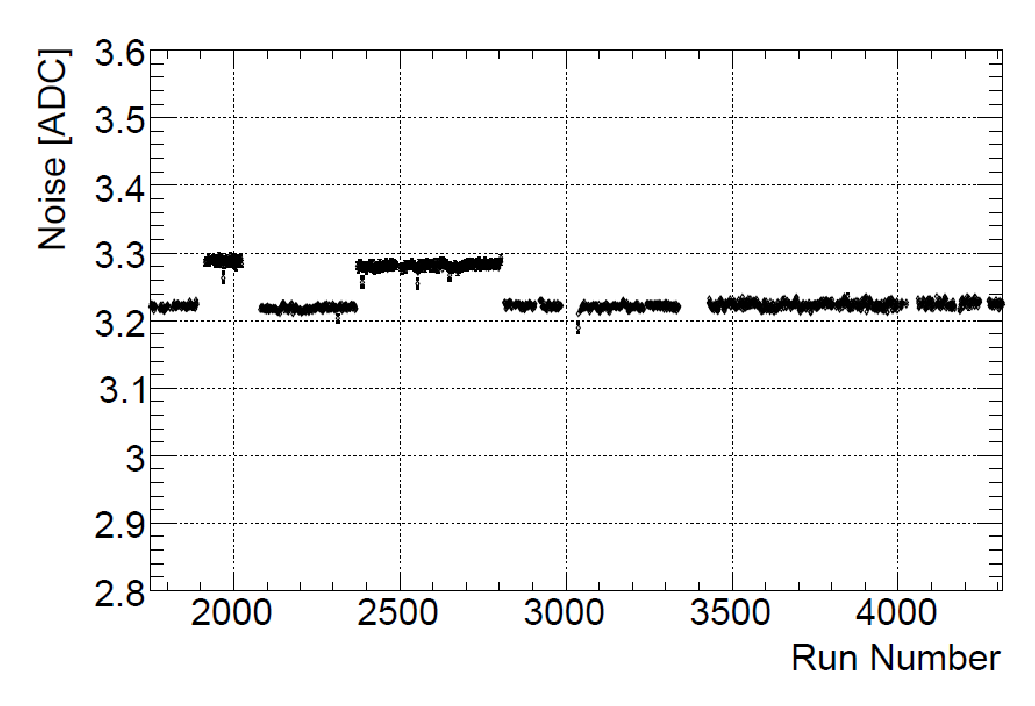
\includegraphics[width=0.8\linewidth,angle=0]{TBoverview/noise_v_run.eps}
\end{center}
\caption[Plot showing pedestal RMS vs. run number]{Plot showing variation in the pedestal RMS, as a function of run number (covering the full duration of the beam test). The pedestal RMS is an indication of the level of noise present in the electronics, showing that this varied with time.}
\label{pedestal_variation}
\end{figure}

The default method for modelling noise in the simulation is done during the digitisation step, where the autocorrelation matrix for the noise is retrieved from a database. It is then used to randomly generate the noise contributions that are added to each sample. However, during data taking, the level of electronic noise present was seen to vary, as is shown in Figure~\ref{pedestal_variation}. After the second period of high noise, the source of the problem was discovered and fixed. However, data for different beam configurations (i.e. particle type/beam energy/beamspot location) were taken at various times, so the average noise present for data taken with a given beam configuration (e.g. 200GeV pions at 4L) differs from that present in data taken with a different beam configuration (e.g. 10 GeV pions at 4L). To account for this effect in the simulation, randomly triggered data (taken from the same runs as the physics data) are used to determine the amount of noise that is added into the simulation, using a procedure that will be discussed below. This method allows different beam configurations to be simulated with different levels of noise, whereas the default method of noise generation would apply the same level of noise to all simulation results, and this noise would not include correlations between channels.


%
%
%
%
%
%The default method for modelling this noise is done during the digitisation step, where a randomly generated noise contribution is added to each sample. 
%
% The default method for applying this noise is to add a random amount 
%
%The default method for modelling this noise is done during the digitisation step, where a randomly generated noise contribution is added to each sample. 
%
%In addition to physics data, some randomly triggered events were recorded during data taking. 
%
%
%Noise can be quantified by studying the rms of the pedestal values, which gives a value of of 3.2 ADC counts per sample when averaged over all channels and all runs. In addition to physics data, some randomly triggered events were recorded during data taking. The data taken by these random triggers is essentially all noise, and allows the correlations between samples to be studied. 
%
%
%
%
%
%Default: noise autocorrelation retrieved from database, which is used to randomly generate the noise that is added to each sample. 
%
%
%However, during data taking the level of electronic noise present was seen to vary, as can be seen from the pedestal values in Figure~\ref{}.
%Runs for different beam configurations done at various times, so average noise present for specific particle/beamspot/energy will be different to that for another beam configuration. 
%To account for this, randomly triggered data taken from same runs as the physics data is used to generate noise added into the simulation, using a procedure discussed below. Default method generating noise lacks this functionality.
%
%
%
%
%
%noise observed to vary
%
%
%
%
%after event simulated, reconstruction done the same way as data, with some exceptions
%First, LarDigitMaker used to simulate electronics and turn hits into digits., which are then fed to LarRawChannelMaker.
%second is the way in which noise is handled. noise needs to be simulated in Monte Carlo. By default, this is done in digitisation, random amount added to each sample. Testbeam case this is not done, instead the noise is added to the LArRawChannelBuilder algorithm.  

\subsection{Noise Generation and Application}


%As data-taking progressed, the level of noise observed in the FCal electronics was seen to vary from %run to run. \red{cause?}. Data for a different sets of run conditions (beam energy, particle type, beamspot position) taken with different level of noise present. 
%
%The RMS of the electronics noise over all runs is 3.2 ADC counts per sample for summed channels \red{and unsummed attenuated channels}. The simulation initially used this value when modelling the electronics noise during the digitisation process, by adding or subtracting a random amount to each sample. However, as the level of the noise varied during data taking it was decided that the simulation should model this, and that the noise used in the simulation should reflect the noise present in the data.
%
%For a given set of data, e.g. 200GeV electrons at position 4L, data taken from randomly triggered events is used to calculate the properties of the electronics noise and model this in the simulation. The random data is used to generate a covariance matrix, describing the correlations between channels


The noise added into the simulation is derived from the randomly triggered data. A covariance matrix is generated by running over the randomly triggered data taken with a specific beam configuration (e.g. 200 GeV pions at position 4L), such that 
\begin{equation}
M_{ij} = \frac{1}{N_\mathrm{events}}\sum_n^{N_\mathrm{events}} e_{i,n} \, e_{j,n}
\end{equation}
where $e_{i,n}$ is the noise reconstructed from the $i$-th channel of the $n$-th event, in ADC counts. The matrix $M_{ij}$ is then diagonalised, such that it can be written as
\begin{equation}
\mathbf{M} = \mathbf{U}^T \, \mathbf{D} \, \mathbf{U}
\end{equation}
where $\mathbf{U}$ is a unitary matrix with columns equal to the eigenvectors of $\mathbf{M}$, and $\mathbf{D}$ is a diagonal matrix which has the eigenvalues of $\mathbf{M}$ as its entries. The matrix $\mathbf{U}^T$ thus acts as a transformation matrix, transforming information from the ``channel'' basis to the eigenvector basis. The eigenvectors and eigenvalues are written to a file, and then retrieved during the reconstruction.

The noise is applied in the LArRawChannelBuilder algorithm, after the pulse peak has been found through application of the OFCs. \cmt{sensible, as this method makes no use of information on individual samples.}The matrix elements $U_{ij}$ and eigenvalues $D_{ii}$ are first read from file. For each event a vector of noise, $N_i$ is then generated. This is done in the eigenvector basis using a normal distribution, such that $\sigma (N_i) = D_{ii}$. This noise is then transformed back into channel basis, such that 
\begin{equation}
N^\prime_i = \sum_j U_{ij} \, N_j
\end{equation} 
which builds in all the correlations between channels. The noise $N^\prime_i$ is then added to the reconstructed pulse peak of the $i$-th channel.

The default method relies on an autocorrelation matrix, such that a correlations between samples are present but each channel is considered independently. The alternative method described above avoids dealing with the noise on individual samples and instead considers the total noise on the reconstructed pulse peak, while also incorporating correlations in the noise between different channels. These correlations are significant, as without them the estimations of the noise contribution in a given cluster are too low. This is important when studying the energy resolution of the FCal, which will be discussed later.


%
%
%
%
%
%
%
%
%
%
%
%
%store eigenvectors and eigen values. (check this).
%
%in ChannelBuilder, vector of noise generated in eigenvector basis. This vector is then multiplied by matrix of eigenvectors in order to transform back into the channel basis. noise then applied to each channel.
%
%method ensures that correlations in noise between channels are preserved, which does not happen in default method. Initial attempts at implement noise only focused on using the correct RMS for each channel, neglecting correlations. Clustered noise was subsequently found to be too low.
%
%
%
%diagonal
%
%   



%\chapter{Testbeam Results}
%\label{chap_TB_results}

%v1.1.
%todo:
%add some of the MC studies in, relate Tb03 to TB04
%mention 98,99 testbeams also
%electron plot of clustered energy vs clustering radius
%maybe more cluster moment plots?



% pion topocluster plots, data and MC (appendix) - need to make both.
%noise vs beam plots - think these are sorted

%more discussion of simulation
%energy loss upstream/refer to JP's thesis
%
%check weights/relative energy amounts.

%\red{some kind of overview}

\clearpage
\section{Event Selection}
\label{sec_event_selection}
The three scintillators located on the adjustable table (labelled S1, S2, and S3 in Figure~\ref{fig_TB_beamline}) were used for triggering. Coincident signals were required from all three in order for the event to be accepted. Any signal from the veto counter indicated that the beam particle had scattered off the upstream material, and in these cases the event was rejected. When analysing data taken from electron beams, events were rejected if there was any signal in either the tail-catcher or the muon counter, as this implied that a muon was present in the event. Showering electrons should have been fully contained within the FCal, so any energy present in the tail-catcher was attributed to muons. It is possible for muons to be produced during hadronic showers, and so these cuts were not applied to data taken from pion beams. 

A series of ``Beam Cleaning'' cuts were also applied, which used information from the scintillators as well as the BPCs. These are intended to remove events in which  multiple beam particles were present and events in which the beam particle had scattered off the upstream material. In order to remove events in which multiple particles were present, the signal from each scintillator was compared to that expected for a minimum ionising particle (MIP). If a single scintillator produced a signal consistent with 5 times that of a MIP, or at least two scintillators gave signals over twice the MIP threshold, the event was rejected. 

While the primary purpose of the BPCs was to provide tracking information on the beam particles, they were also used in the beam cleaning in a similar way to the scintillators. A key feature of MWPCs is that the total charge arriving at an anode is proportional to the total number of electron-ion pairs produced in the chamber, and from this the number of ionising particles that passed through the active areas could be inferred. Events were rejected if a single BPC produced a signal five times greater than that expected for a single MIP, or if at least two BPCs generated a signal twice that expected for a single MIP.


%BPCs used to reconstruct track. fit made in xz and yz plane, and event rejected if chi2 (40) is bad (indicating a particle that has scattered). 

%These tracks were then used to make ``beam envelope'' cuts, which were intended to remove events containing undesired particles. The magnet systems in the H6 beamline tended to place electrons and hadrons into different areas of phase space, due to differences in their charge to mass ratios.


% The $x$ intercept of the track is measured from the BPC closest to the FCal, and an "ideal" slope (in the $x-z$ plane) is determined for a track of the desired particle type which has the intercept. This procedure is then repeated in the $y-z$ plane. For each direction, the difference between the measured track slope and the ideal track slope is computed. The sum of the squares of these differences are then computed, and if this total exceeds a specified threshold the track is deemed to lie outside the beam envelope, and the event is rejected.

Particle tracks were reconstructed by performing a linear fit to the data from the BPCs. The $x-z$ and $y-z$ planes were reconstructed separately, with the BPCs providing six measurements of the track in each plane. If the sum of the $\chi^2$ values for these fits exceeded 40.0 (for 8 degrees of freedom), the event was rejected. The reconstructed tracks were then used to define ``beam-envelope'' cuts, which were intended to remove events containing undesired particles. The beams delivered to the testing area were not completely pure, and so hadrons were sometimes present in the electron beams and protons sometimes present in the pion beams. The magnet systems in the H6 beamline tended to separate electrons and hadrons into different areas of phase space, due to differences in their charge to mass ratios. The $x$ intercept of the track, $c_x$, was measured using the BPC closest to the FCal (``BPC 5''). This intercept was then used to determine an ``ideal'' slope in the $x-z$ plane for the desired particle type, $m_{x,\mathrm{ideal}}(c_x)$, as well as a width parameter, $\Delta m_x (c_x)$. Similarly, the intercept $c_y$, was used to define an ideal slope, $m_{y,\mathrm{ideal}}(c_y)$, and width, $\Delta m_y (c_y)$, in the $y-z$ plane.
%
% procedure is then repeated to obtain the intercept, ideal slope, and width parameter in the $y-z$ plane, denoted as $c_y$, $m_{y,\mathrm{ideal}(c_y)$, and $\sigma_y (c_y)$ respectively. 
% 
The quantity 
\begin{equation}
\Delta S = \left(\left( \frac{ m_{x,\mathrm{ideal}}(c_x) - m_{x,\mathrm{measured}} }{ \Delta m_x (c_x)} \right)^2 + \left( \frac{ m_{y,\mathrm{ideal}}(c_x) - m_{y,\mathrm{measured}} }{ \Delta m_y (c_y)} \right)^2 \right)^{1/2}
\end{equation}
was then calculated, where $m_{x,\mathrm{measured}}$ and $m_{y,\mathrm{measured}}$ are the measured track slopes in the $x$ and $y$ directions, respectively. The quantity $\Delta S$ describes how much the measured track direction deviates from the ideal track direction for the desired particle type. If $\Delta S$ exceeded a specified threshold (1.25 in this analysis), the measured track was deemed to lie outside the beam-envelope for the desired particle type, and the event was rejected. 
%Particle trajectories and the beam envelope from a 193 GeV electron run are plotted in Figure~\ref{envelope_fig}.

%%%%%%%%%%%%%%%%%%%%%%%%%%%%%%%%%%%%%%%%%%%%%%%%%%%%%%%%%%%%%%%%
%\begin{figure}[!htbp]
%\begin{centering}
%\subfigure{
%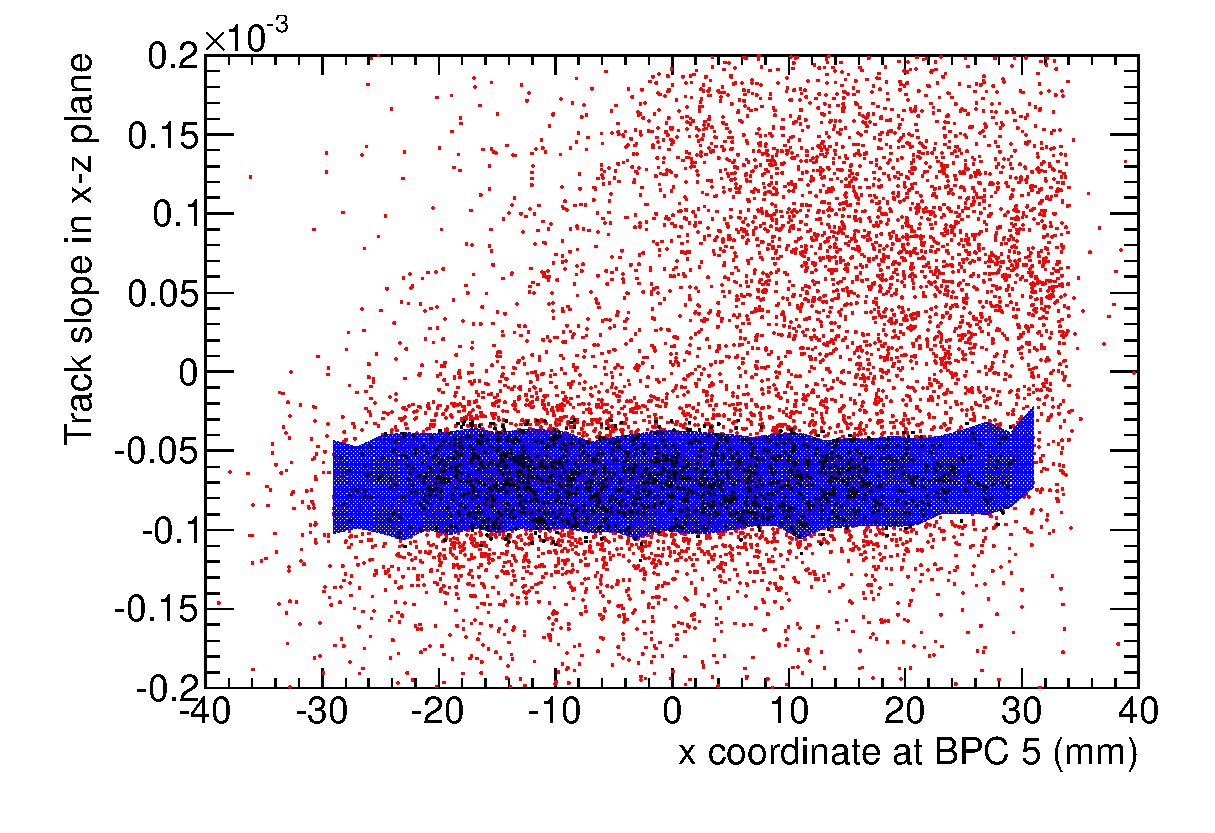
\includegraphics[width=0.45\linewidth,angle=0]{FCalTB_plots/tracks_x_e_run2324.eps}
%\label{envelope_fig_x}
%}
%\subfigure{
%
%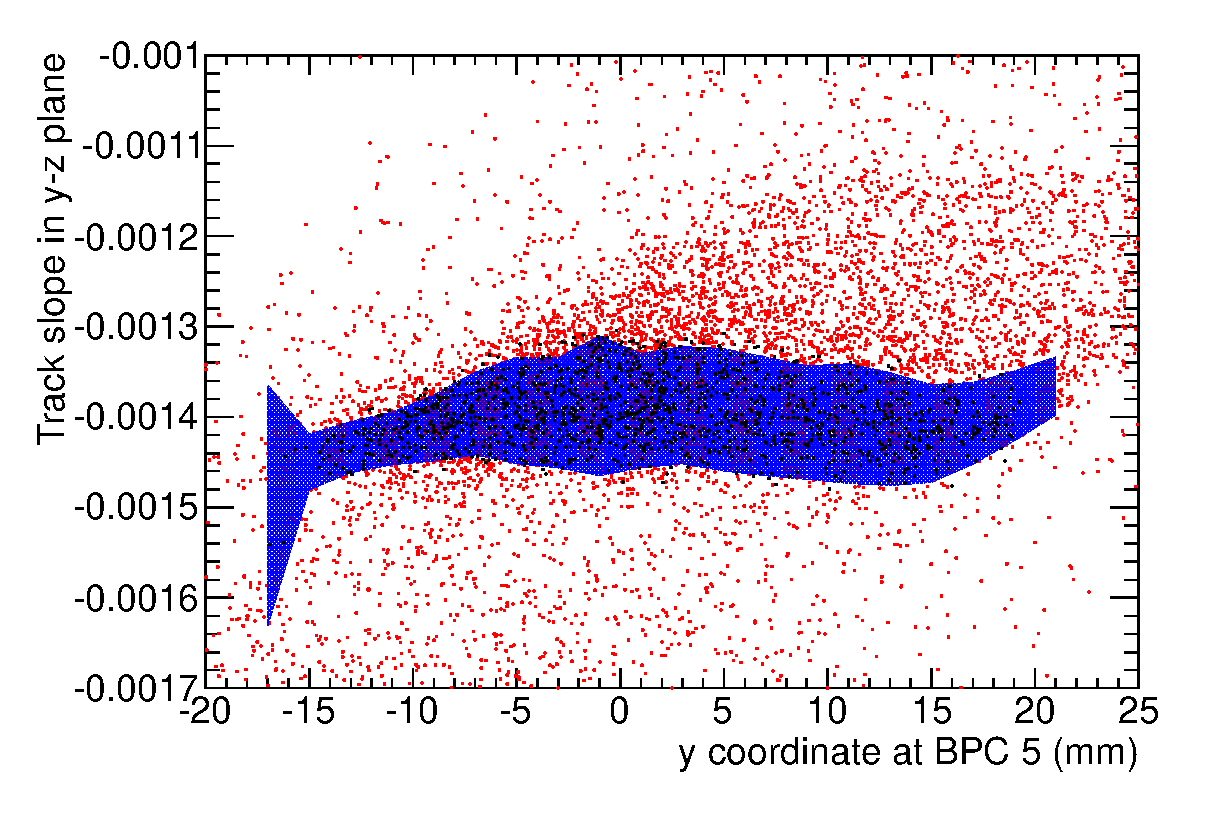
\includegraphics[width=0.45\linewidth,angle=0]{FCalTB_plots/tracks_y_e_run2324.eps}
%\label{envelope_fig_y}
%}
%\caption{Particle trajectories in the $x-z$ plane (left) and the $y-z$ plane (right), taken from a 193 GeV electron run at position 4L. The region shaded in blue corresponds to the beam envelope, while the black (red) markers correspond to tracks that pass (fail) the envelope cut. Note that a track must lie within both envelopes in order to pass the beam envelope cut. } 
%\label{envelope_fig}
%\end{centering}
%\end{figure}
%
%%%%%%%%%%%%%%%%%%%%%%%%%%%%%%%%%%%%%%%%%%%%%%%%%%%%%%%%%%%%%%%%


As mentioned in Section~\ref{sec_TBoverview_timing}, two TDCs were used to measure the time interval between the trigger signal and the clock pulse from the TTC, at which time the signals from the calorimeter were sampled. Output from the TDC is given as an integer number of TDC counts, between $\sim 300$ and $\sim 800$, which covers a time interval of 25 ns and thus gives the TDC a time resolution of 50 ps. There are three regions where a mismeasurement of the TDC can be problematic: near the TDC's minimum value, its maximum value, and in the ``wrap-around'' region. The wrap-around point is where the phase jump occurs, such that the time interval measured by a TDC jumps suddenly from 0 ns to 25 ns. The TDC phase quality is defined as the smallest difference between the TDC reading and one of the problematic regions. Event timing was determined using the TDC which had the highest phase quality. Events were rejected in cases where the readout from the highest quality TDC was within 1 ns of a problematic region.
% The event was rejected if the TDC phase quality did not lie in the range 20 $<$ TDcPhaseQuality $<$ 230, as in these cases the better clock choice was still within 1 ns of a problematic region.
%} %not stoked about this

%An additional timing cut was implemented using $\tau$, the time of the pulse peak as reconstructed by the OFCs (c.f. equation~\ref{eq_ofc_AT}. 
%
%
%halfling cut goes here.

The CEDAR detector (described in Section~\ref{sec_TBoverview_beamline}) was also used to improve the beam purity. It was mainly used to eliminate proton events when analysing data taken with $\pi^+$ beams, by rejecting events containing beam particles that the CEDAR did not identify as charged pions. However, the CEDAR information was also used when analysing electron data at 60~GeV, as the electron beams had a low purity at this energy.

%
%also another cut.
%
%The TDC Phase Quality is defined as the 
%
%
%
%Timing cut. 











%The measured slope is then compared to the ideal slope, and the procedure is repeated in the $y-z$ plane. For each direction, the difference between the ideal and measured track slopes in each direction are then summed in quadrature. and if the sum exceeds a specified threshold 
%
%it's chi^2 in track slope.
%
%The same thing is done in the $y$ direction, and in each case the deviation of the measured track from the ideal track is computed.  The difference between the actual track slope and the ideal track slope is then computed, and the process is repeated in the $y-z$ plane
%Beam envelope cuts? they work how?
%
%look at closest bpc to FCal
%if based on it's position, determine ideal slope for this intercept
%envelope of slopes determined around this. difference between actual slope and ideal slope determined. If the significance of this difference exceeds some threshold, event is cut.
%
%actual slope is "allowed" to be 
%
%
%Timing cuts.






%The BPCs were also 
%
%
%Beam cleaning
%- remove multiple particles and those that are scattered
%remove impurities from beam
%
%S1 S2 S3 signal over mip signal
%also BPCS - same deal
%
%
%
%CEDAR used on electron runs to remove pions, and on pi+ runs to remove protons.
%
%Beam envelope cuts - BPCS give good measurement of particle tracks - straight line fit to determine position and direction
%Cut if quality of fit is shit(?)
%Also used beam envelope. (Check this again) particles with different charge/mass ratios tend to occupy different regions of phase space in (x,v). Tracks are analysed, envelopes are defined for pions and electrons. Reject event if track isn't within envelope, or is too far outside it.
%
%
%
%timing - halflings?
%clustering timing cut.
%TBphase quality cut




\section{Results Obtained Using Cylindrical Cell Clustering}

\subsection{Analysis of Electron Data}
\label{TB_results_electrons}
%events taken with electron and positron beam, polarity determined by other experiments
%
%no. of triggers?
%
%final events after all cuts
%
%response plotted goes here

%\red{fancy timing cut should go somewhere}









%
%What is the deal with the beam polarity, exactly. 
%
%cuts used as described earlier. CEDAR is off, except at 60~GeV where its hard to get a good, pure beam.

Using the tracking information from the BPCs, the point at which the beam particles strike the front face of the calorimeter can be determined (with accuracy on the order of 1 mm). Cylindrical clusters are then formed by collecting all cells within a certain distance of the impact point. For the analysis of data taken with electron beams, only calorimeter cells in FCal1 are considered. For the analysis of data taken with hadron beams, calorimeter cells from all three FCal modules are included in the cylindrical cluster. As the FCal was oriented at an angle with respect to the incoming beam particles, the beam particle track is projected through the FCal to give a slightly different impact point for each module. This impact point changes by $~\sim2$cm between neighbouring modules.

%Cylindrical clusters are then formed by summing the energy of each cell within a certain radius of this impact point. A clustering radius of 8 cm is used for analysis of the electron data. 
%
%
%The Moliere radius is a quantity used to describe the transverse development of electromagnetic showers. It is given by \blue{blah}, and on average $\sim 90\%$ of the shower energy is contained within a cylinder of radius $\sim R_M$. \cmt{can cite paper on my desk by fabiola and fabjen, calorimetery in particle physics, reviews of modern physics}.
%either do this here or in detector chapter, where Moliere is first mentioned
%
%

On average, about 80-90\% of the energy deposited by an electromagnetic shower is contained within a cylinder of radius $\rho_M$ (the \moliere radius). In FCal1 the \moliere radius is about 17~mm, and $\sim 99\%$ of the energy is contained within a cylindrical cluster of radius 8 cm, as can be seen in Figure~\ref{TBplot_electron_radials}. Clusters with radii 12~cm and 16~cm are also generated during event reconstruction. These larger clusters capture about 1\% more energy than the 8~cm cluster, however the noise contained within the cluster increases by $\sim50 \%$ at a radius of 12~cm and  $\sim100 \%$ at a radius of 16~cm. For this reason 8~cm clusters are used in the analysis of electron data. Note that both positron and electron beams were available during the beam test. No distinction was made between these particles during this analysis, and so both particles will be referred to as ``electrons'' in this Section\footnote{The distinction between electrons and positrons is made later in this Section during some of the discussion on systematic effects, but this is the only case in which they are treated separately}. 



%%%%%%%%%%%%%%%%%%%%%%%%%%%%%%%%%%%%%%%%%%%%%%%%%%%%%%%%%%%%%%%
\begin{figure}[tb]
\begin{centering}
\subfigure{
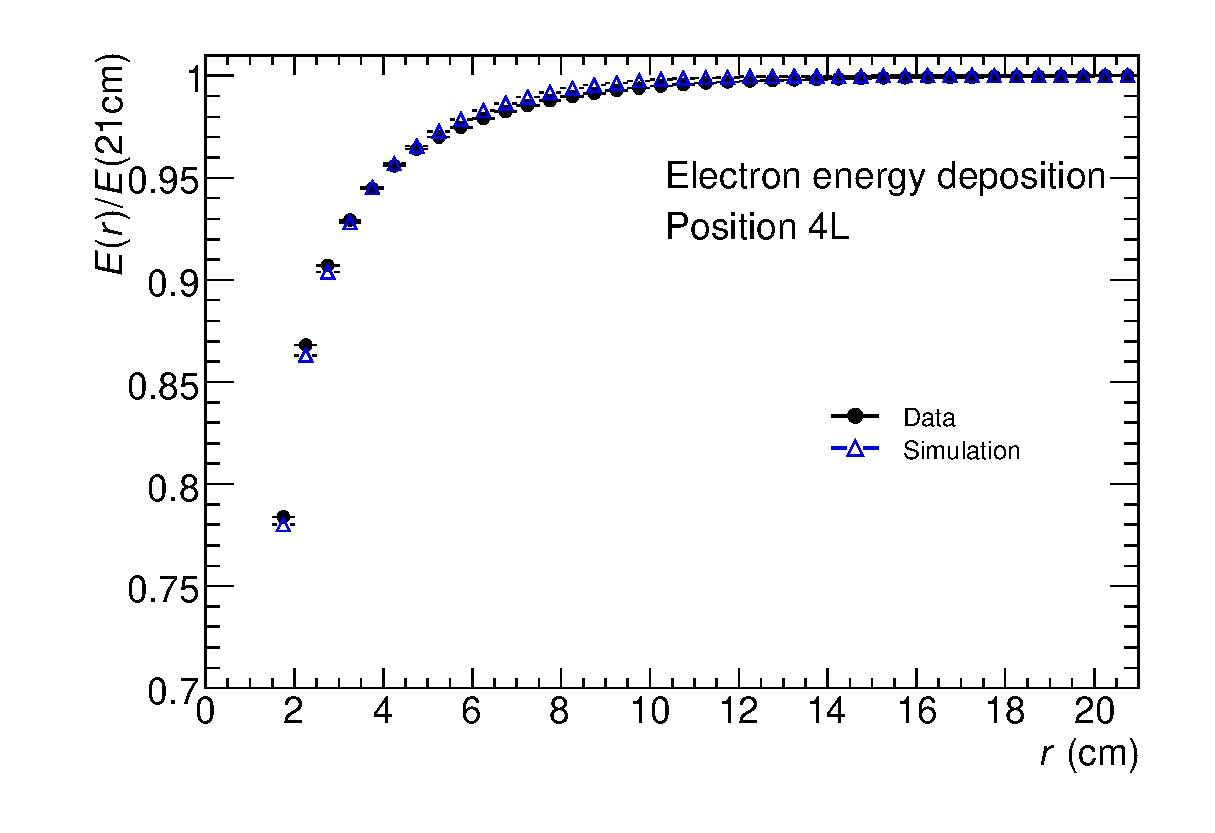
\includegraphics[width=0.45\linewidth,angle=0]{FCalTB_plots/radial_electrons_4L_193GeV_int.eps}
\label{TBplot_electron_rad_4L_int}
}
\subfigure{

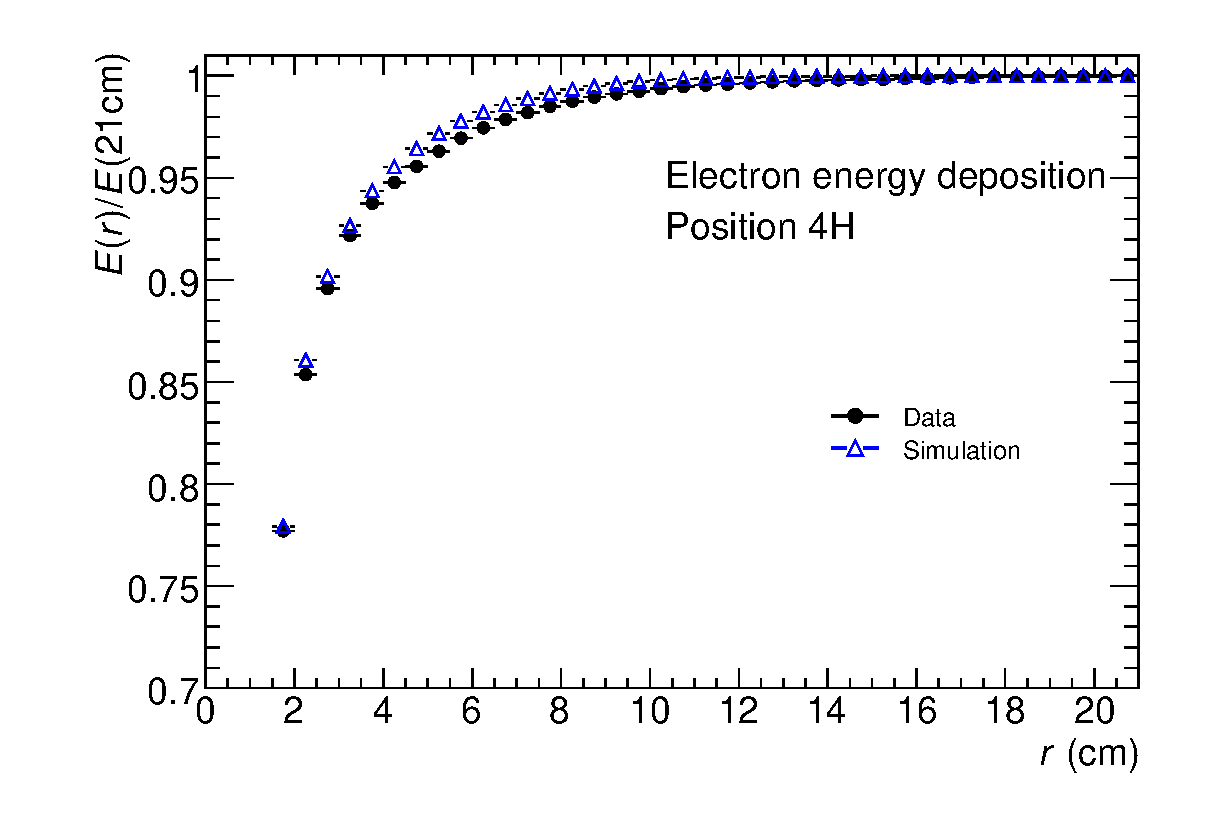
\includegraphics[width=0.45\linewidth,angle=0]{FCalTB_plots/radial_electrons_4H_193GeV_int.eps}
\label{TBplot_electron_rad_4H_int}
}\\
\subfigure{
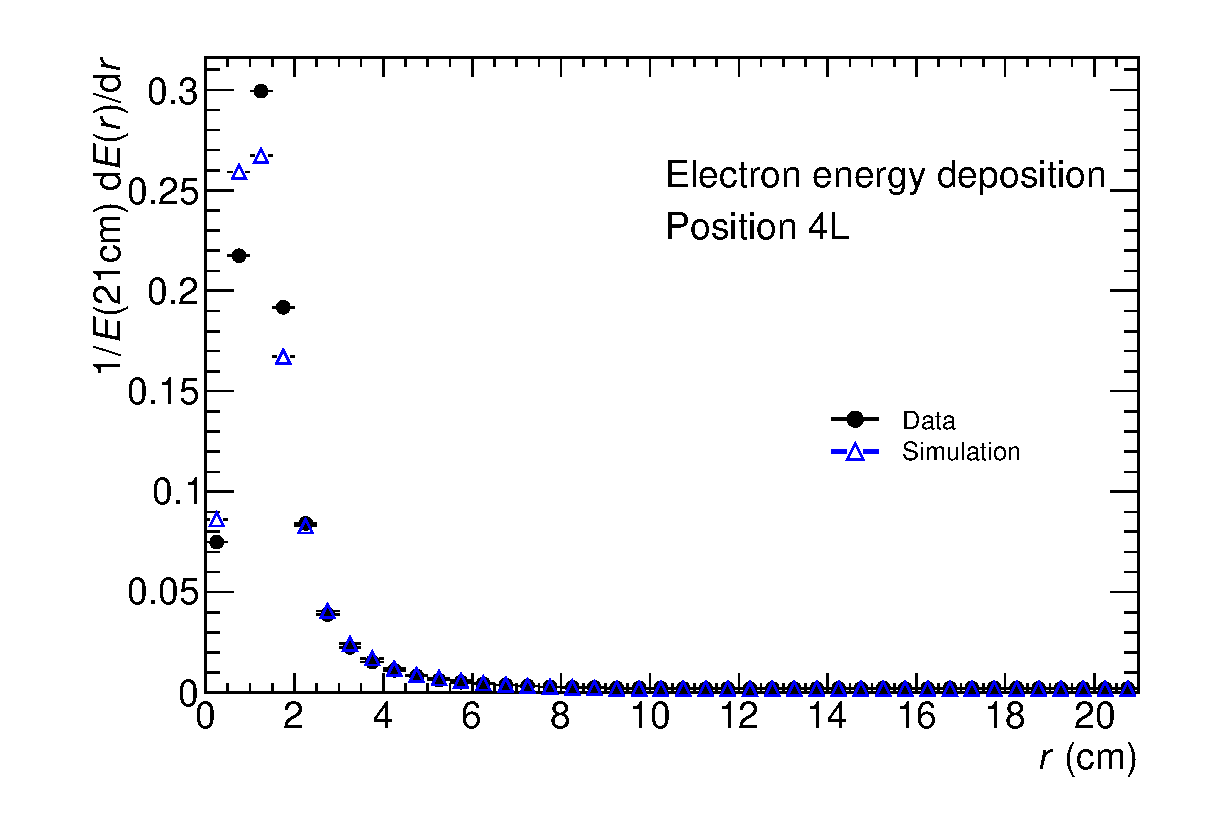
\includegraphics[width=0.45\linewidth,angle=0]{FCalTB_plots/radial_electrons_4L_193GeV_diff.eps}
\label{TBplot_electron_rad_4L_diff}
}
\subfigure{

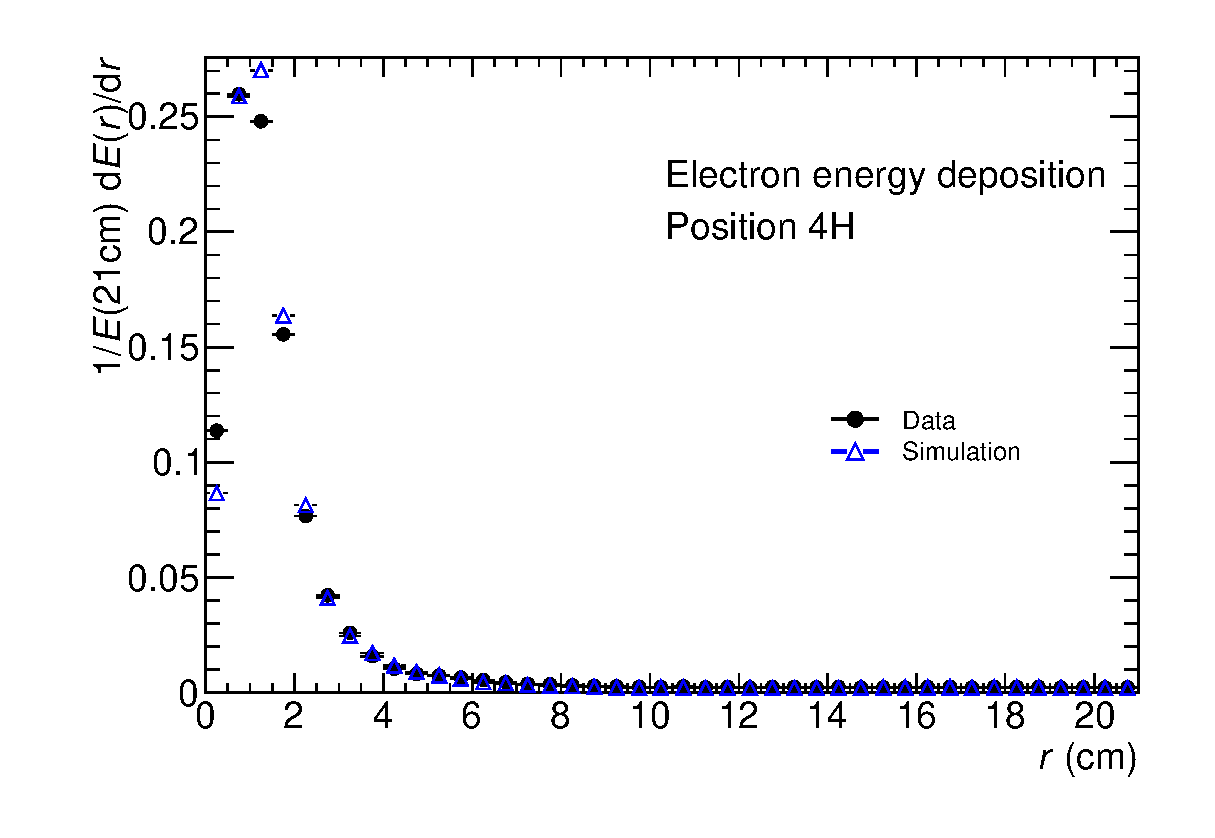
\includegraphics[width=0.45\linewidth,angle=0]{FCalTB_plots/radial_electrons_4H_193GeV_diff.eps}
\label{TBplot_electron_rad_4H_diff}
}
\caption[Radial distribution of the energy deposited by electrons]{Fraction of energy contained within a cylinder of radius $r$ centred on the beam impact point. Figures~(a) and (b) show the fraction of energy contained within a cylinder of radius $r$ compared to a cylinder of radius 21cm, for showers initiated by 193.1~GeV electrons at position 4L and 4H, respectively. Figures~(c) and (d) show the fractional energy deposited between $r$ and $r+\ud r$ as a function of $r$, for position 4L and 4H respectively. The value of 21cm was chosen because as cylinders of larger radii are not entirely contained within the FCal. } 
\label{TBplot_electron_radials}
\end{centering}
\end{figure}

%%%%%%%%%%%%%%%%%%%%%%%%%%%%%%%%%%%%%%%%%%%%%%%%%%%%%%%%%%%%%%%



%\red{halflings}

%. The BPCs present in the beamline are used to obtain the trajectory of the beam particle, which is then projected to a point on the front face of the FCal1 module. A cluster is then created by summing the energy of all FCal1 channels within 8cm of the impact point. 

The energy reconstructed for a given particle has some dependence on the position at which that particle impacts the calorimeter, as an electron striking the centre of an electrode rod deposits less visible energy in the calorimeter than one that hits close to the liquid argon gap \cite{TB93_prototype,TB98_electron_signals}. As the diameter of the beamspot (65 mm) is an order of magnitude larger than the spacing between adjacent electrodes (7.5 mm in FCal1), many different impact points are sampled. This leads to a non-Gaussian distribution in the response, as this is essentially the sum of many different Gaussian distributions. A good fit to the data is obtained using a double Gaussian function,

\begin{equation}
F(E) = a_0 \exp \left( - \frac{(E - a_1)^2}{2 a_2^2} \right ) +  a_3 \exp \left( - \frac{(E - a_4)^2}{2 a_5^2} \right)
\label{eqn_dbl_Gaussian}
\end{equation}
%where $A_i$, $\mu_i$, and $\sigma_i$ are the peaks, means and widths of the component Gaussians. The mean response is then found by taking the first moment of $F(E)$, such that
where the parameters $a_0$ and $a_3$ describe the amplitudes, $a_1$ and $a_4$ describe the means, and $a_2$ and $a_5$ describe the widths of the component Gaussians. 
%$A_i$, $m_i$, and $\sigma_i$ are the amplitudes, means and widths of the component Gaussians, respectively. 
When fitting the response distributions with the double Gaussian, some constraints are imposed on the parameters. The non-Gaussian shape of the response is determined by the geometry of the calorimeter, as this determines which impact points are closer to a liquid argon gap (yielding a higher response), and which impact points are further from the gap (giving a lower response). This suggests that the shape of the response should be independent of the beam energy, which allows some constraints to be imposed on the fit parameters in equation~\ref{eqn_dbl_Gaussian}. The ratios of the populations and the means of the two Gaussians are held fixed, such that
\begin{eqnarray}
\frac{a_0 a_2}{a_3 a_5} & = & C_1 \label{eqn_constraint_1}\\
\frac{a_1}{a_4} & = & C_2,
\label{eqn_constraint_2}
\end{eqnarray}
where $C_1$ and $C_2$ are constants obtained from an unconstrained double Gaussian fit on the 193 GeV electron data (or 200~GeV hadron data). These values are then used to apply constrained fits to the responses at lower beam energies. The constrained fits tend to have better agreement with the peak of the distribution, and so these have been used to obtain the results presented in this chapter, though the unconstrained fits have been considered in systematic studies.
%whereas the unconstrained fits sometimes result in one Gaussian being used to fit the peak while the second is used to fit the tails of the distribution. %\red{constrained and unconstrained usually pretty similar}.
%
%variation in impact point
%variation in response
%due to geometry
%
%two Gaussians used to fit this response
%
%relative populations and means therefore determined by geometry
%independent of energy/constrained.
%
%
%
%
%
%As the variation in the response is due to variations in the beam particle impact point,  These constraints are motivated by the geometry of the calorimeter: as this is responsible for the
%

The mean response, $\bar{E}$, is taken as the first moment of $F(E)$, where the $i$-th moment, $\mu_i$, is given by
\begin{equation}
\label{eqn_moment}
\mu_i = \frac{\int^{E_{\mathrm{max}}}_{E_{\mathrm{min}}}  E^{i} F(E) \ud E }{\int^{E_{\mathrm{max}}}_{E_{\mathrm{min}}}  F(E) \ud E},
\end{equation}
where the limits of the integral, $E_\mathrm{min}$ and $E_\mathrm{max}$, are obtained from the response histogram. The lower limit, $E_\mathrm{min}$, is taken from the low edge of the lowest energy bin that is not empty, while $E_\mathrm{max}$ is the upper edge of the highest non-empty histogram bin. 

The width of the response, $\sigma$, is determined from the first and second moments of $F(E)$, such that
%\begin{equation}
%\mu_2 = \frac{\int^{E_{\mathrm{max}}}_{E_{\mathrm{min}}}  E^2 F(E) \ud E }{\frac{\int^{E_{\mathrm{max}}}_{E_{\mathrm{min}}}  F(E) \ud E},
%\end{equation}
%such that
\begin{equation}
\sigma = \left( \mu_2 - \mu_1^2 \right)^{1/2}.
\label{DG_width_def}
\end{equation}

Statistical uncertainties on these quantities may be written in terms of higher order moments. However, for simplicity, a (single) Gaussian fit is made to the response, and the moments of this Gaussian are used to compute the statistical uncertainties. The statistical uncertainties on $\bar{E}$ and $\sigma$ are then
\begin{eqnarray}
\Delta \bar{E} = \Delta \mu_1 & = & \frac{\sigma_g}{\sqrt{N_g}} \\
\Delta \sigma & = & \frac{\sigma_g}{\sqrt{2N_g}},
\end{eqnarray}
where $\sigma_g$ and $N_g$ are the width and population from the (single) Gaussian fit.




The response of the FCal to electrons (for all beam energies) is plotted in Figures~\ref{TBplot_electron_response_4L_data} and \ref{TBplot_electron_response_4H_data}, for positions 4L and 4H, respectively. The results of the fits to these distributions are summarised in Tables \ref{TBres_table_elec_4L} and \ref{TBres_table_elec_4H}. 
%%%%%%%%%%%%%%%%%%%%%%%%%%%%%%%%%%%%%%%%%%%%%%%%%%%%%%%%%%%%%%%
\begin{figure}[tbp]
\begin{center}
\subfigure{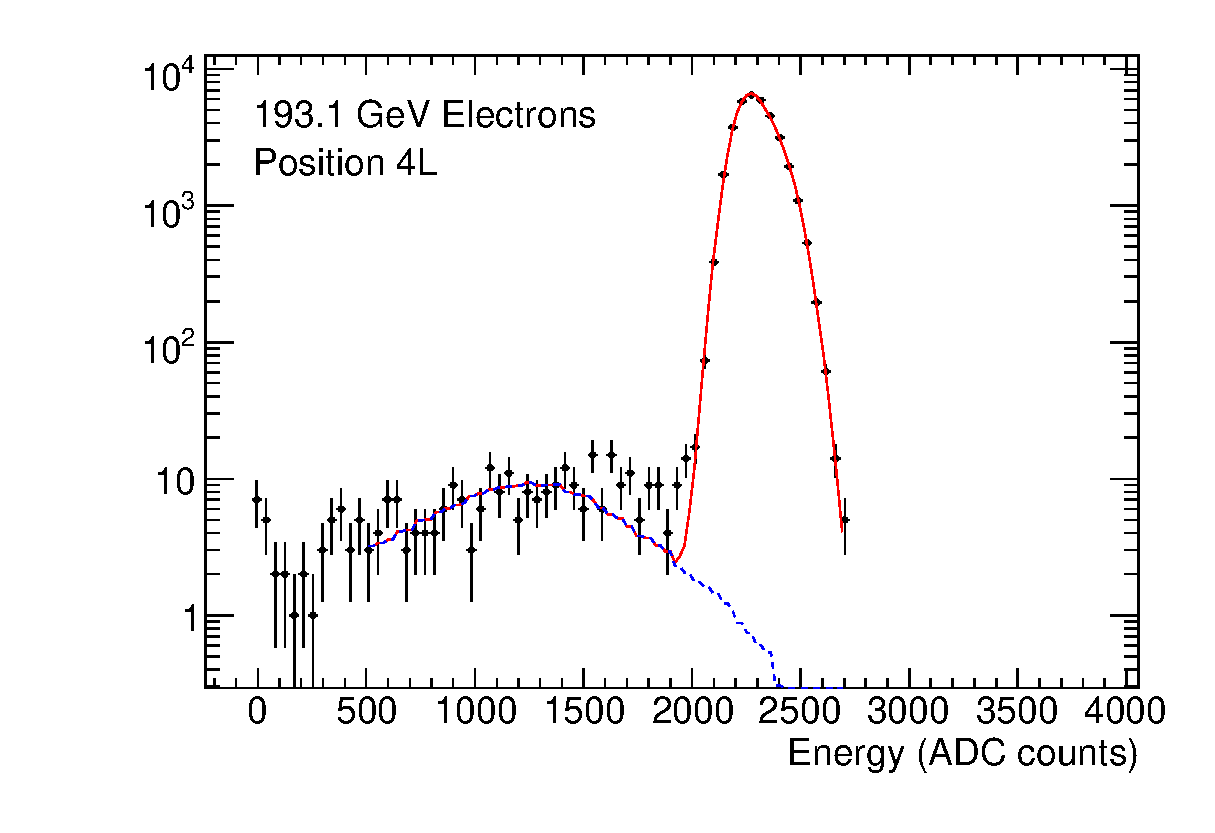
\includegraphics[width=0.45\linewidth,angle=0]{FCalTB_plots/Response_individual_data/Electron_response_193GeV_4L_data.eps}}
\subfigure{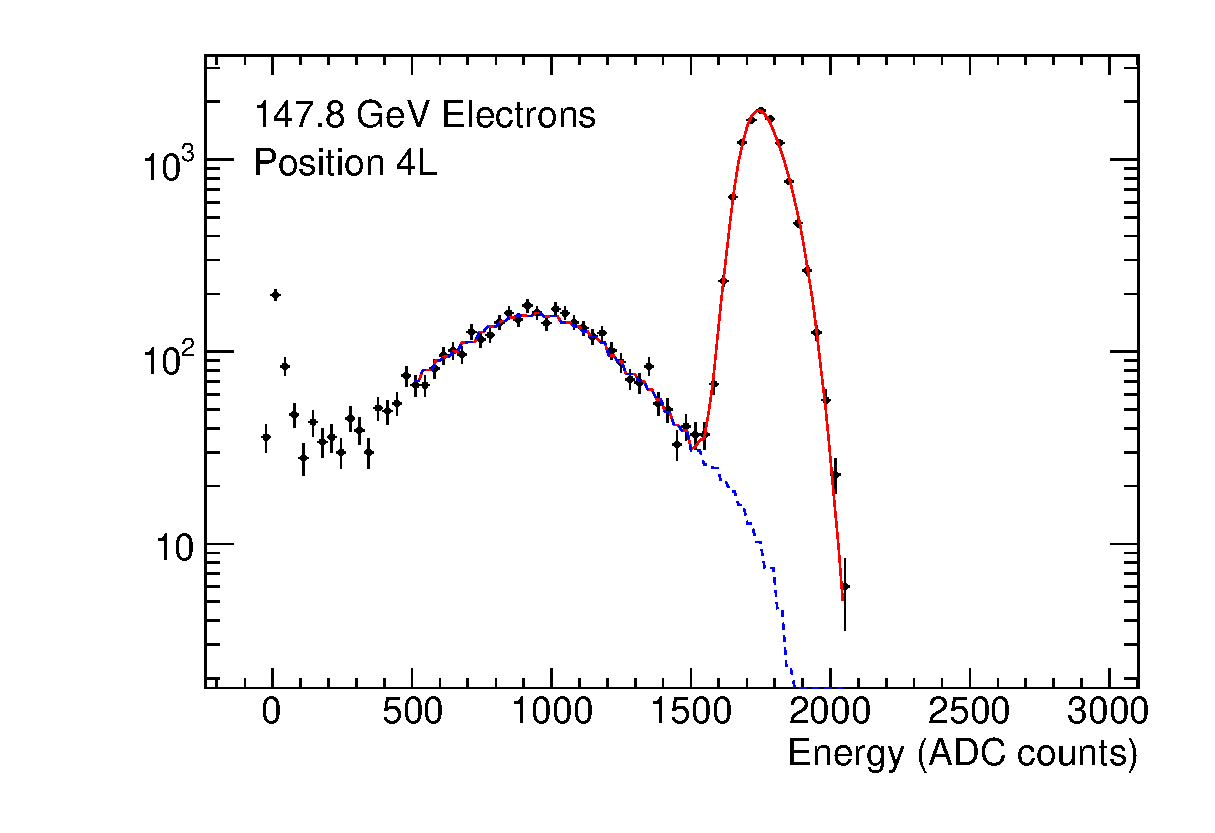
\includegraphics[width=0.45\linewidth,angle=0]{FCalTB_plots/Response_individual_data/Electron_response_148GeV_4L_data.eps}}\\
\subfigure{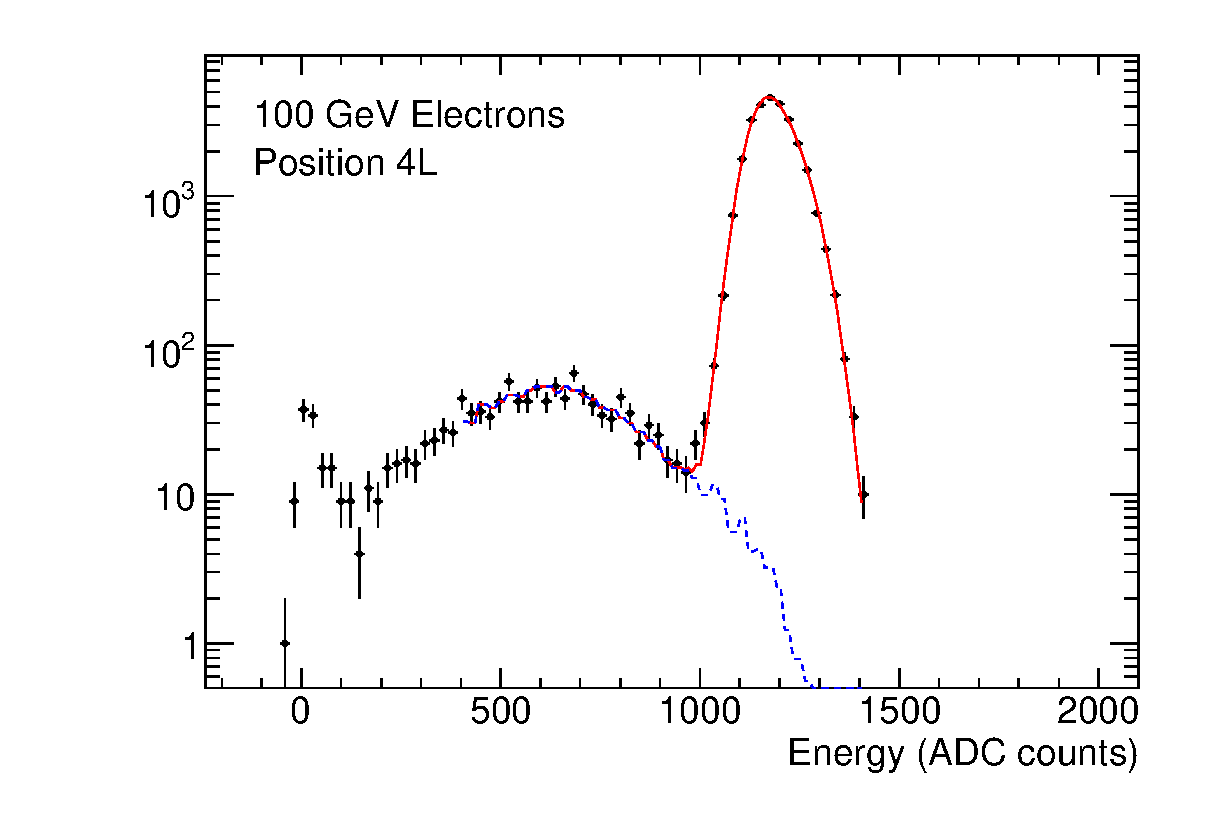
\includegraphics[width=0.45\linewidth,angle=0]{FCalTB_plots/Response_individual_data/Electron_response_100GeV_4L_data.eps}}
\subfigure{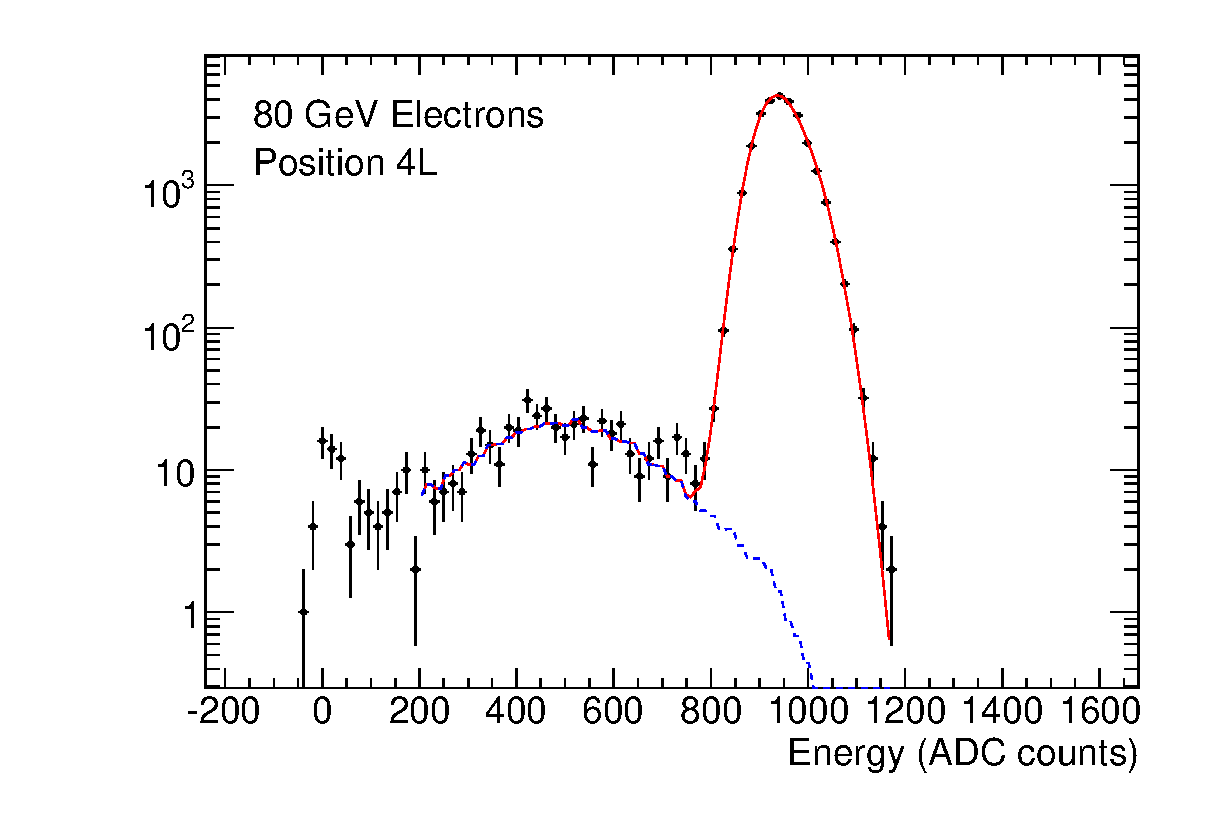
\includegraphics[width=0.45\linewidth,angle=0]{FCalTB_plots/Response_individual_data/Electron_response_80GeV_4L_data.eps}}\\
\subfigure{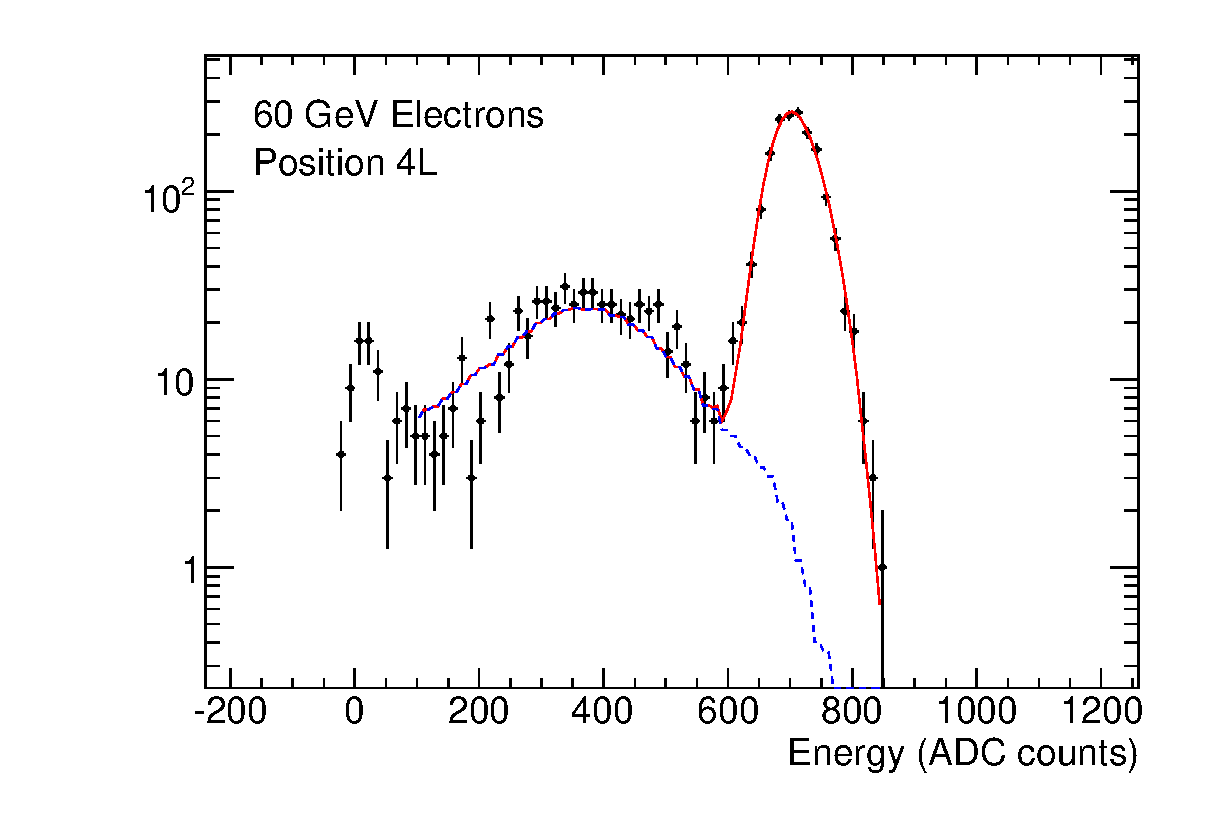
\includegraphics[width=0.45\linewidth,angle=0]{FCalTB_plots/Response_individual_data/Electron_response_60GeV_4L_data.eps}}
\subfigure{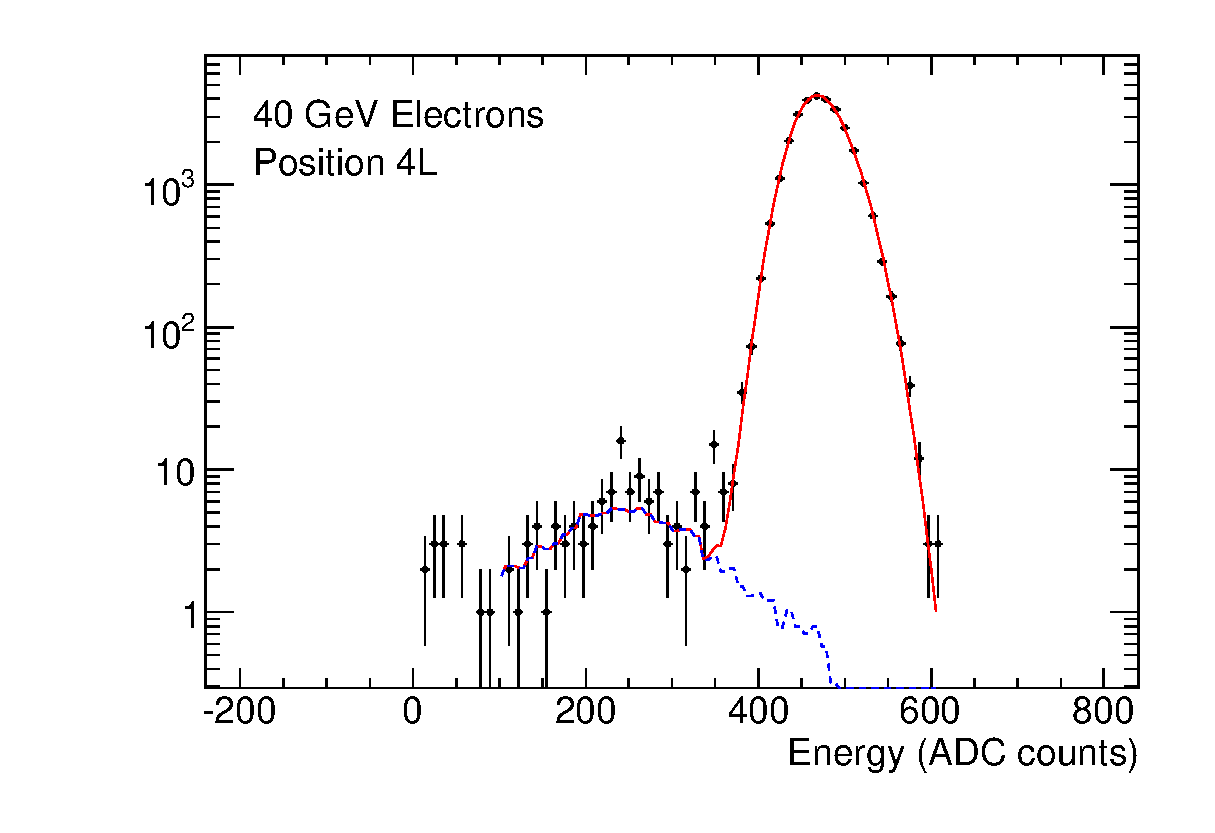
\includegraphics[width=0.45\linewidth,angle=0]{FCalTB_plots/Response_individual_data/Electron_response_40GeV_4L_data.eps}}\\
\subfigure{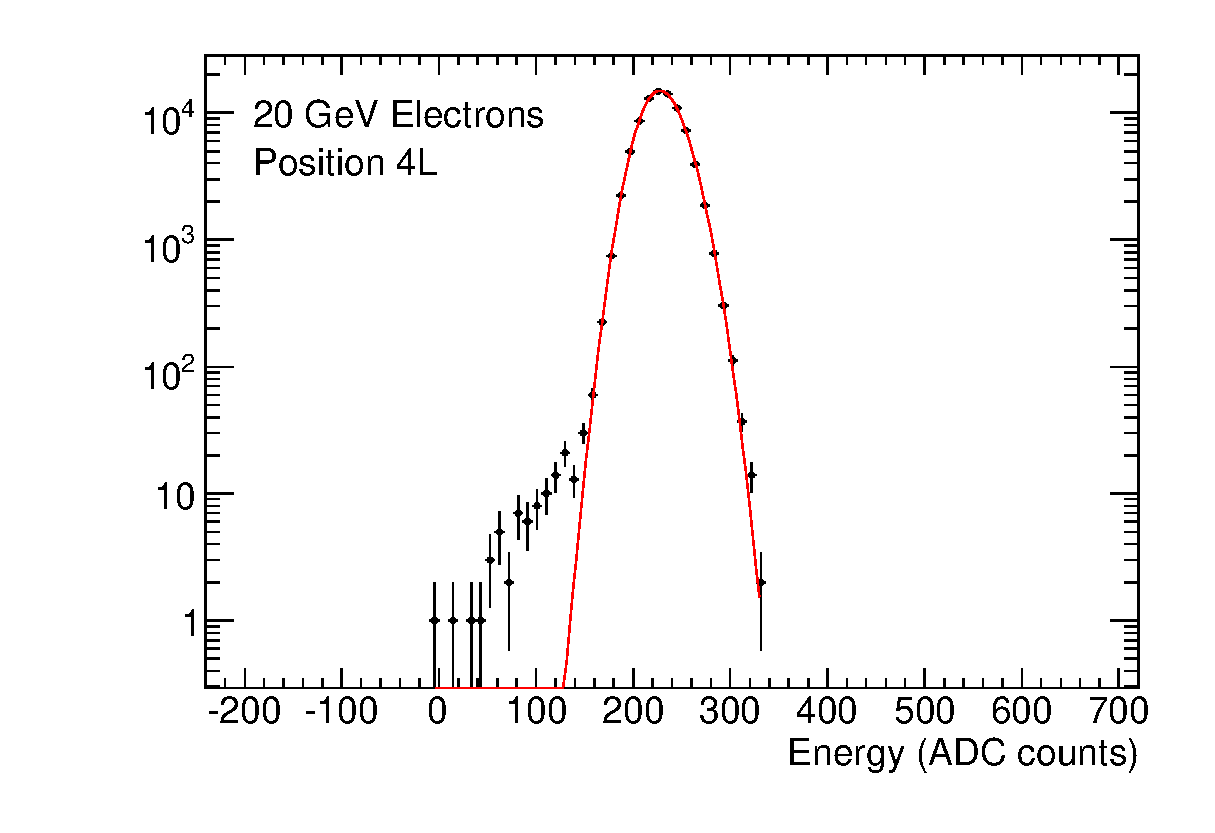
\includegraphics[width=0.45\linewidth,angle=0]{FCalTB_plots/Response_individual_data/Electron_response_20GeV_4L_data.eps}}
\subfigure{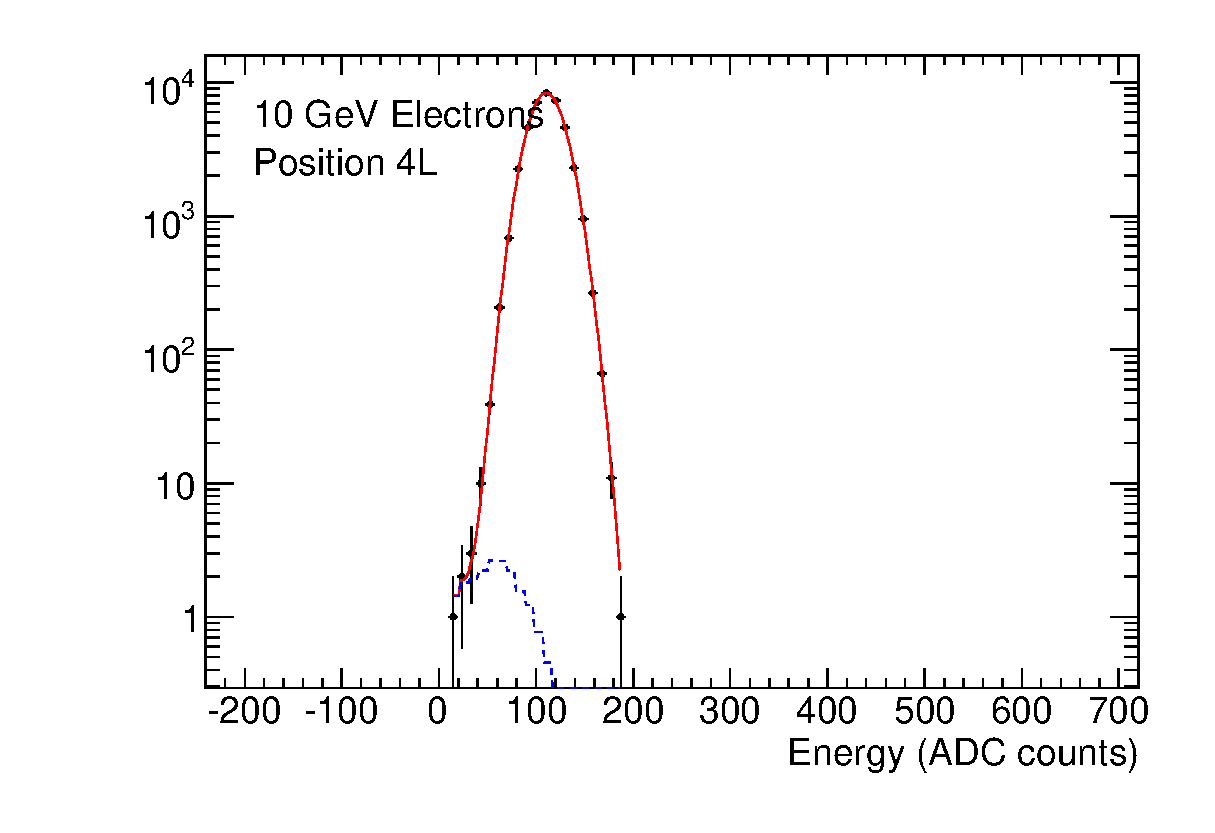
\includegraphics[width=0.45\linewidth,angle=0]{FCalTB_plots/Response_individual_data/Electron_response_10GeV_4L_data.eps}}
\end{center}
\caption[Response of the FCal to electrons at position 4L]{Response of the FCal to electrons at position 4L. The red curve is the total fit to the data, which consists of a double Gaussian fit to the electron peak as well as the fit to the hadron contribution (blue dashed line).}
\label{TBplot_electron_response_4L_data}
\end{figure}






%%%%%%%%%%%%%%%%%%%%%%%%%%%%%%%%%%%%%%%%%%%%%%%%%%%%%%%%%%%%%%%

%%%%%%%%%%%%%%%%%%%%%%%%%%%%%%%%%%%%%%%%%%%%%%%%%%%%%%%%%%%%%%%

%\begin{figure}[!htb]
%\begin{center}
%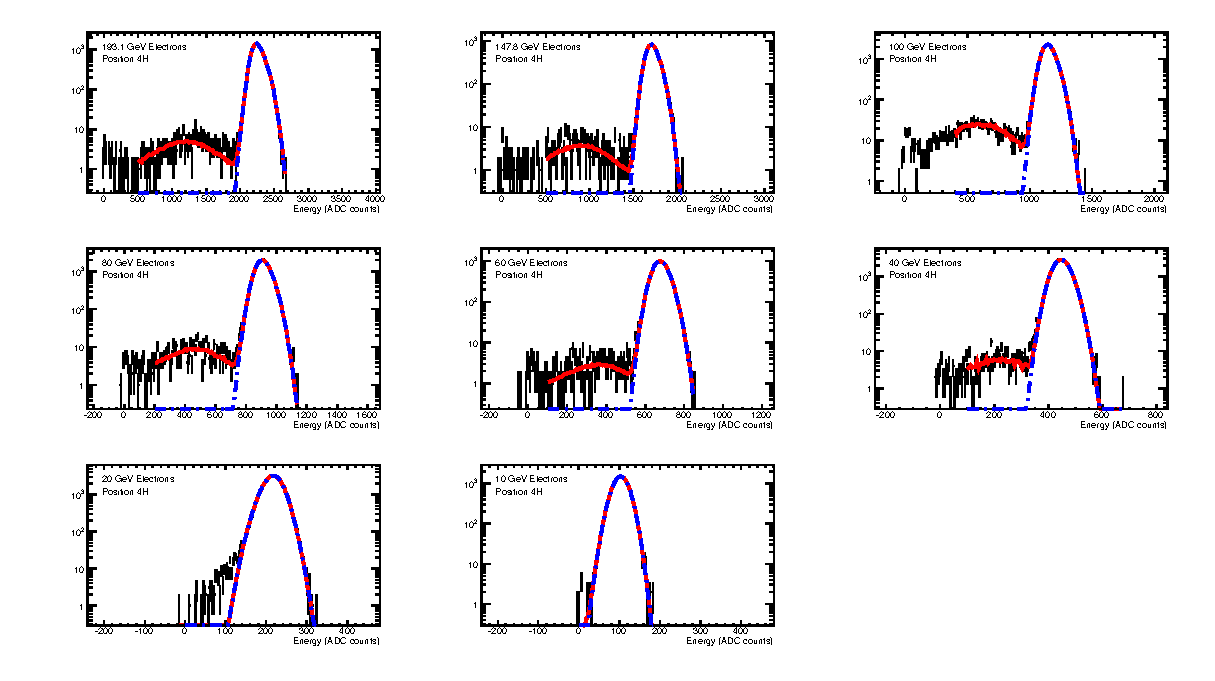
\includegraphics[width=1.0\linewidth,angle=0]{FCalTB_plots/electron_response_4H_data.eps}
%\end{center}
%\caption{Response of the FCal to electron beams at position 4H. The blue dashed curve double Gaussian fit to the electron peak, while the red curve shows the total fit to the electron peak plus the contaminant hadron contribution.}
%\label{TBplot_electron_response_4H_data}
%\end{figure}
%%%%%%%%%%%%%%%%%%%%%%%%%%%%%%%%%%%%%%%%%%%%%%%%%%%%%%%%%%%%%%%%
\begin{figure}[tbp]
\begin{center}
\subfigure{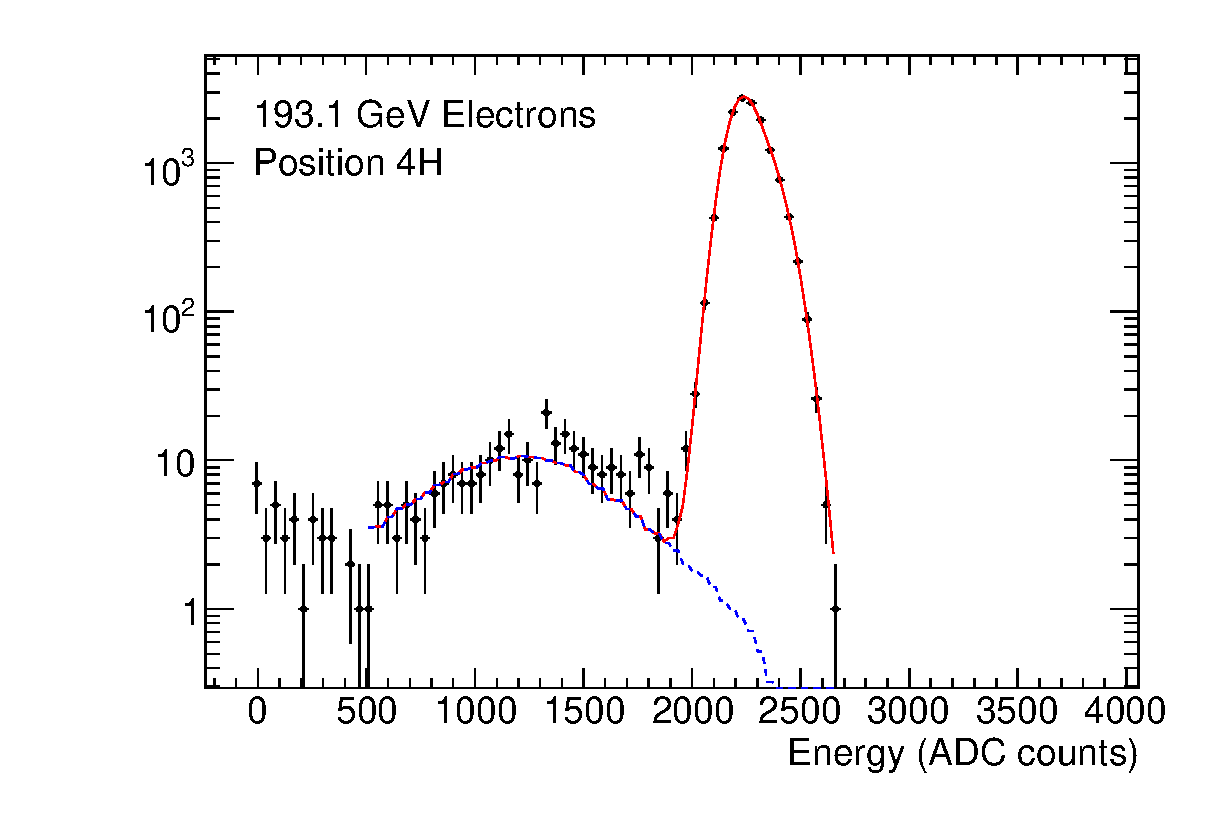
\includegraphics[width=0.45\linewidth,angle=0]{FCalTB_plots/Response_individual_data/Electron_response_193GeV_4H_data.eps}}
\subfigure{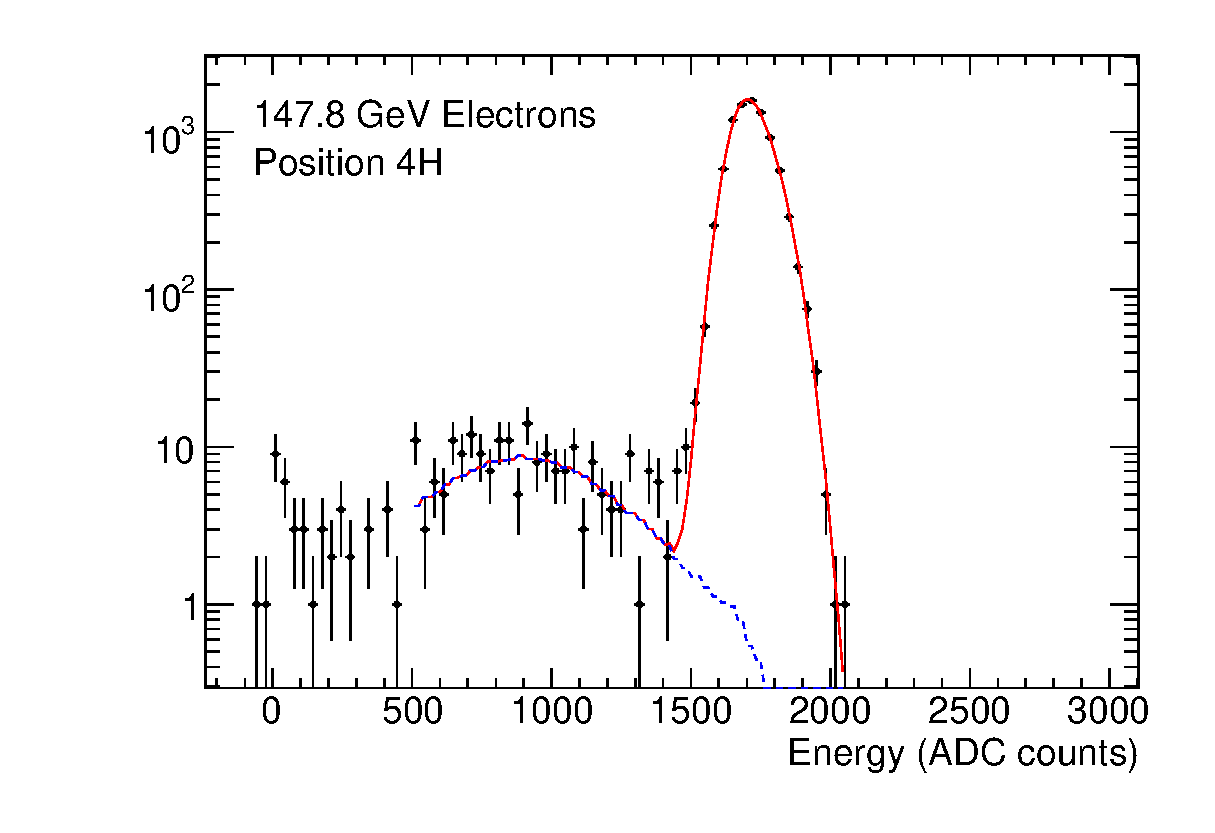
\includegraphics[width=0.45\linewidth,angle=0]{FCalTB_plots/Response_individual_data/Electron_response_148GeV_4H_data.eps}}\\
\subfigure{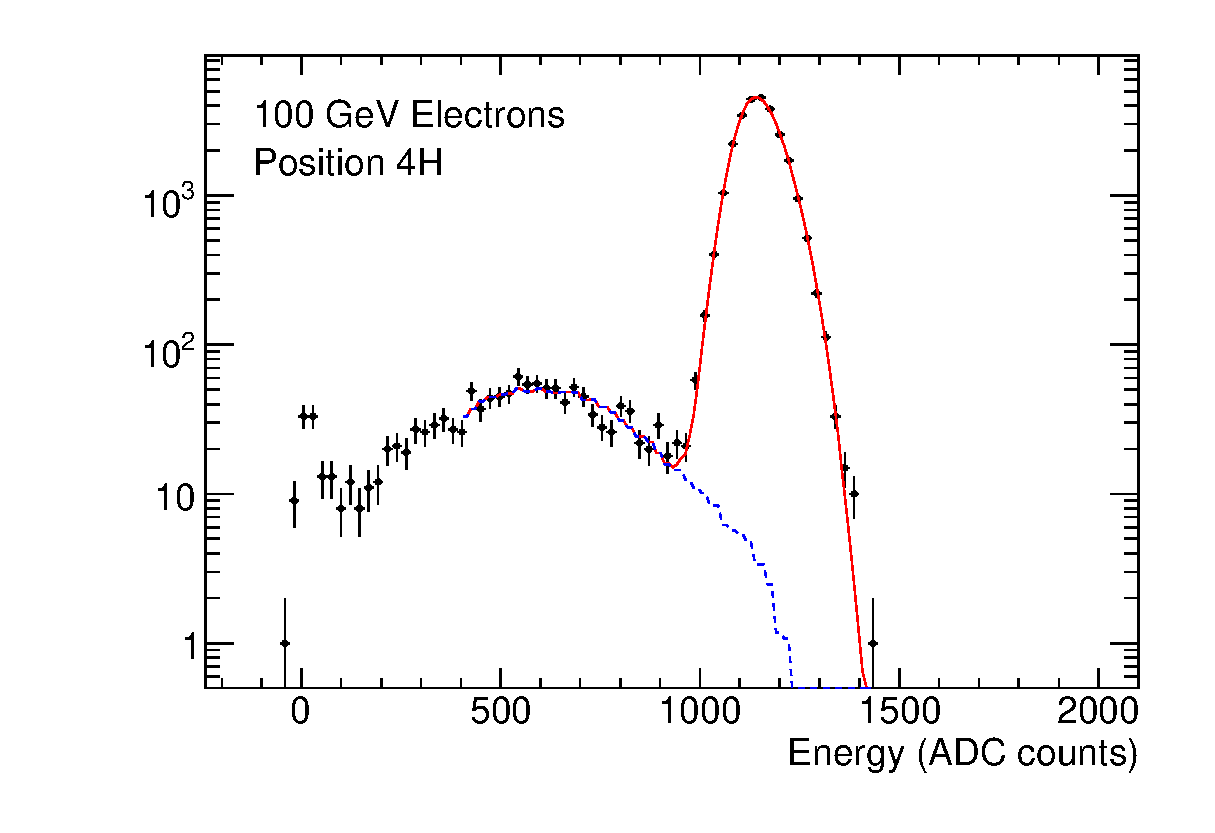
\includegraphics[width=0.45\linewidth,angle=0]{FCalTB_plots/Response_individual_data/Electron_response_100GeV_4H_data.eps}}
\subfigure{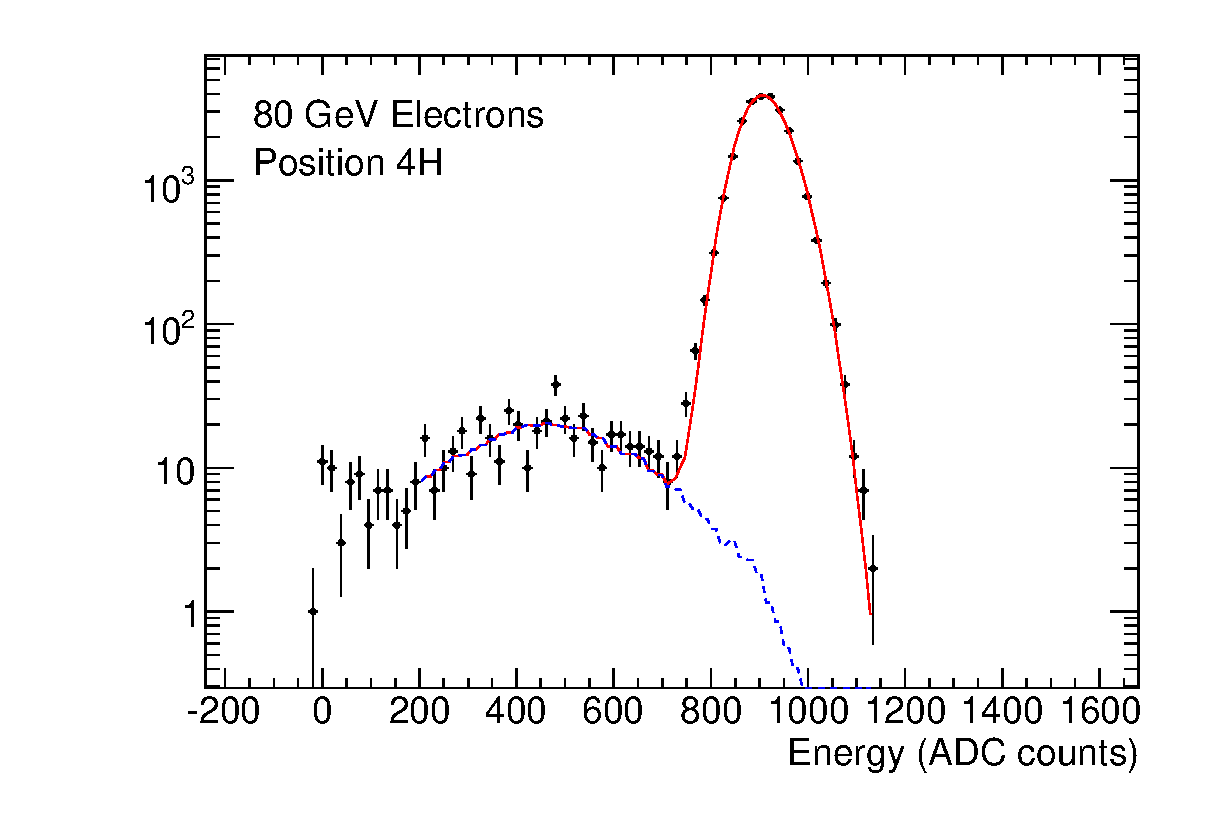
\includegraphics[width=0.45\linewidth,angle=0]{FCalTB_plots/Response_individual_data/Electron_response_80GeV_4H_data.eps}}\\
\subfigure{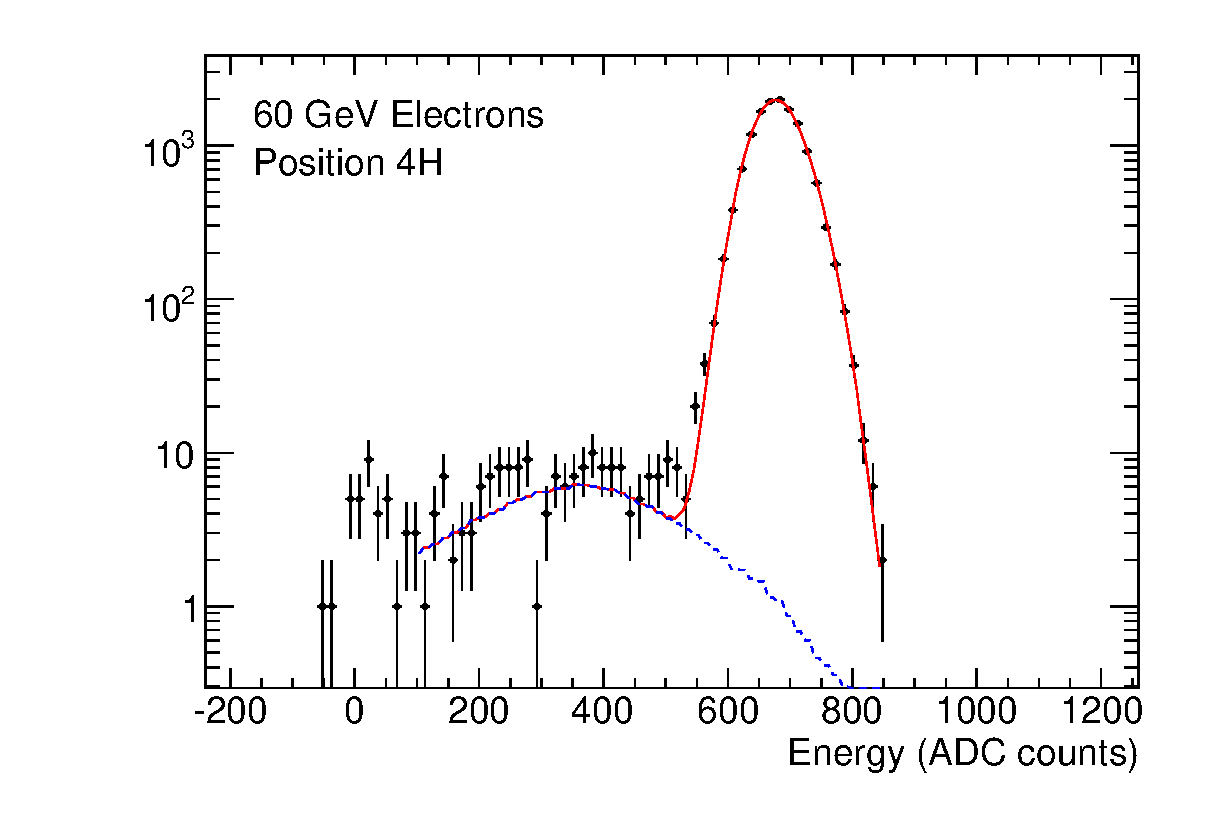
\includegraphics[width=0.45\linewidth,angle=0]{FCalTB_plots/Response_individual_data/Electron_response_60GeV_4H_data.eps}}
\subfigure{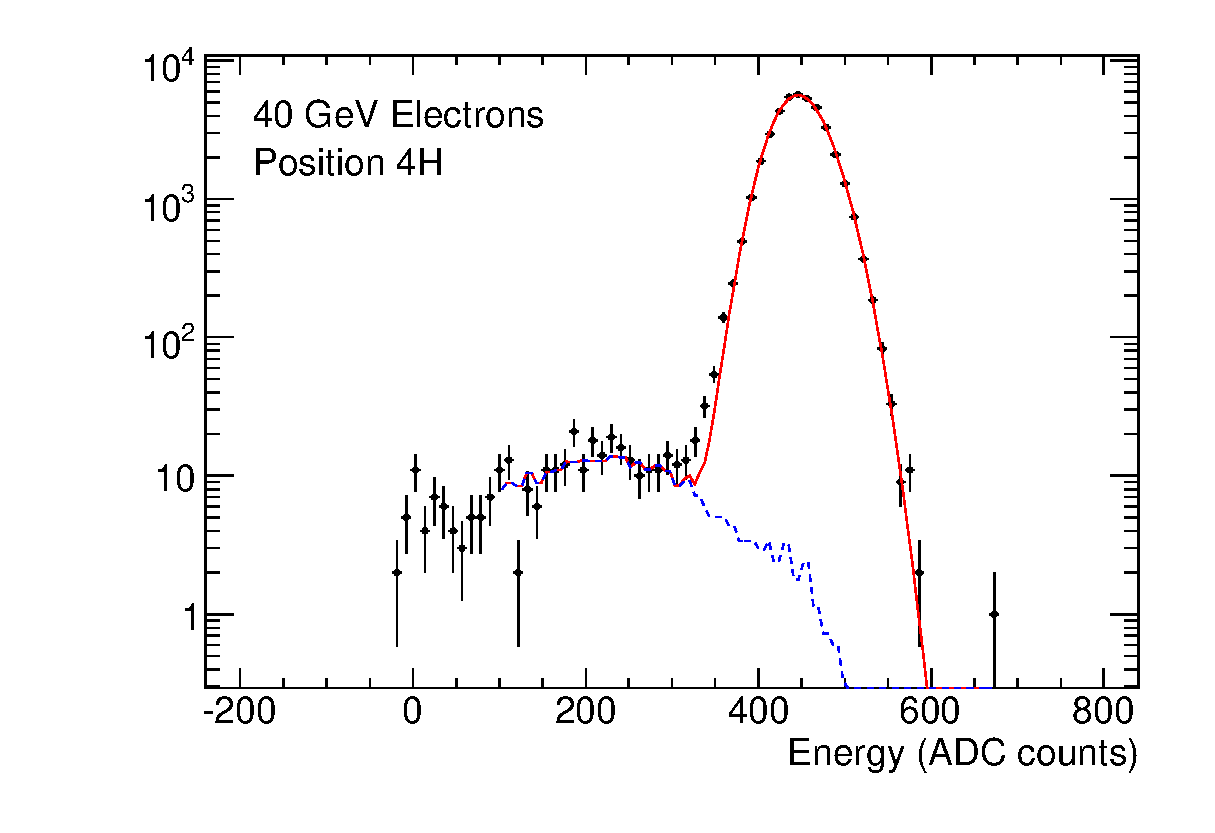
\includegraphics[width=0.45\linewidth,angle=0]{FCalTB_plots/Response_individual_data/Electron_response_40GeV_4H_data.eps}}\\
\subfigure{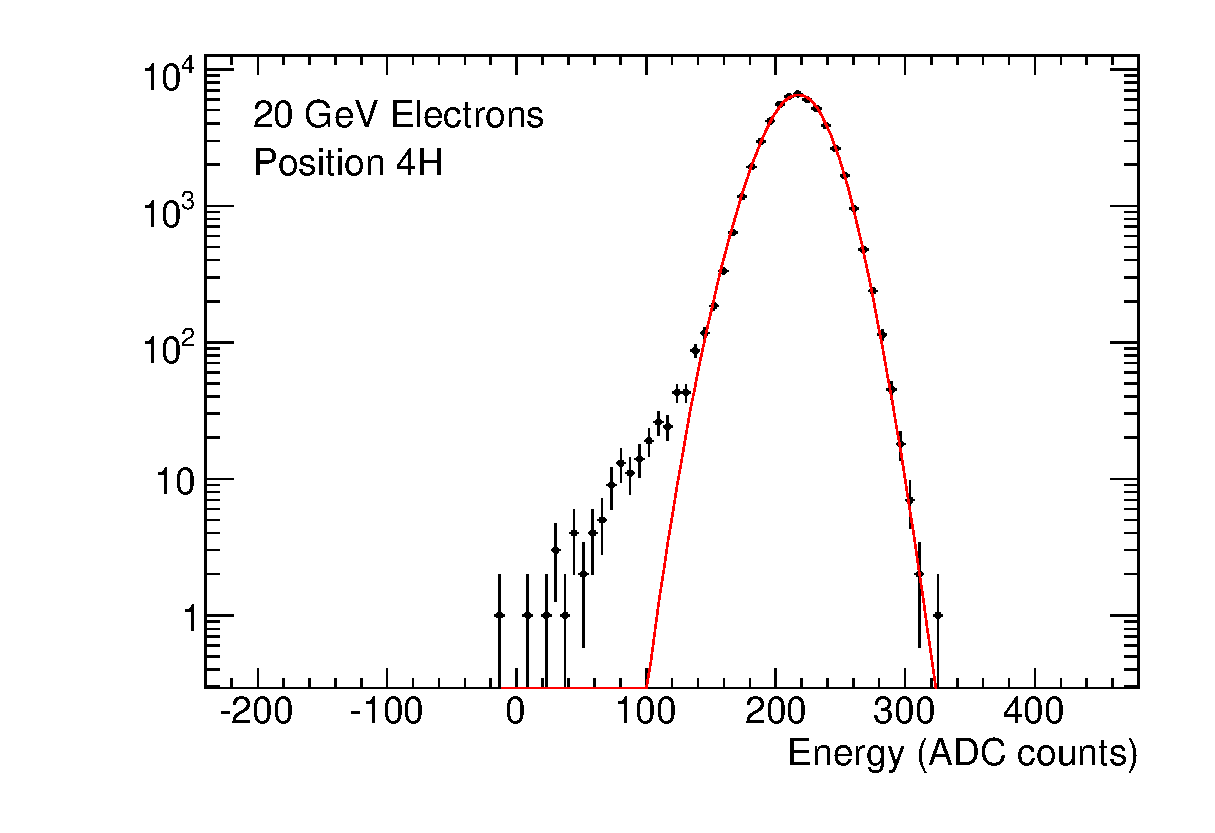
\includegraphics[width=0.45\linewidth,angle=0]{FCalTB_plots/Response_individual_data/Electron_response_20GeV_4H_data.eps}}
\subfigure{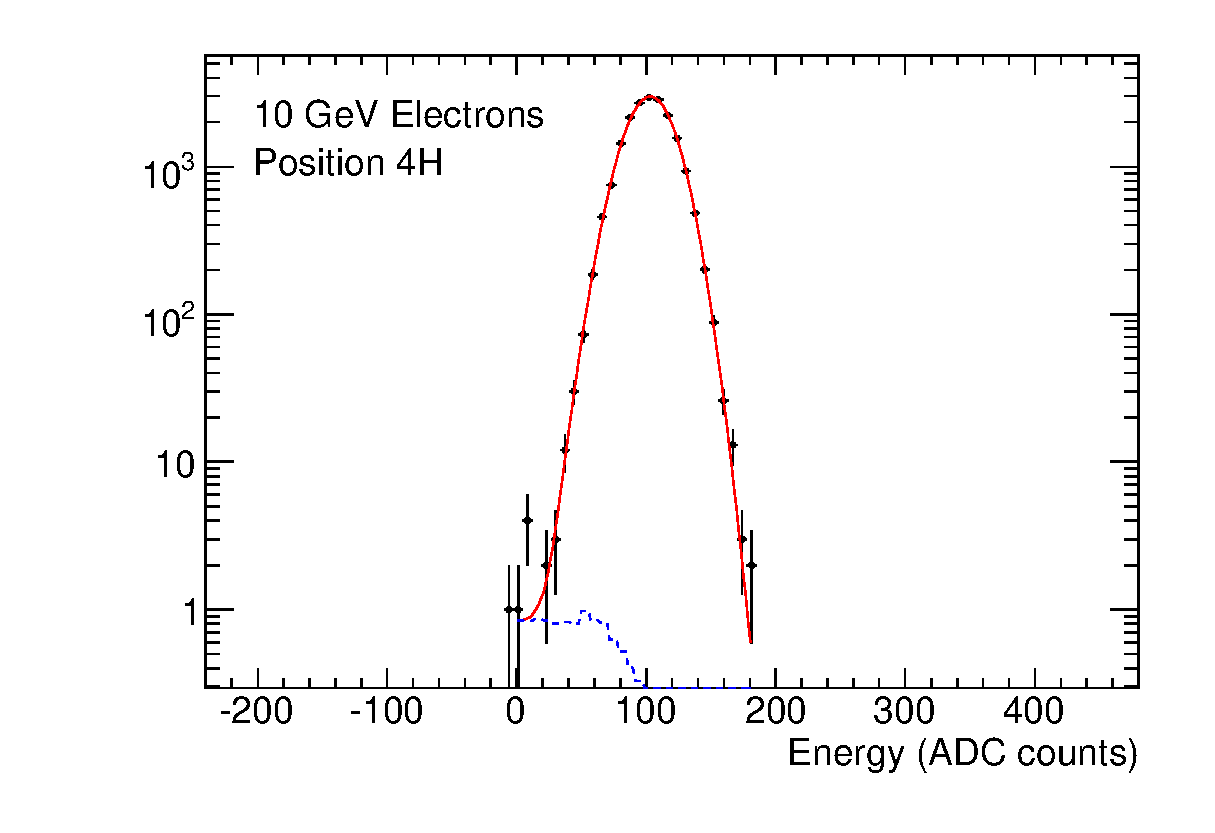
\includegraphics[width=0.45\linewidth,angle=0]{FCalTB_plots/Response_individual_data/Electron_response_10GeV_4H_data.eps}}
\end{center}
\caption[Response of the FCal to electrons at position 4H]{Response of the FCal to electrons at position 4H. The red curve is the total fit to the data, which consists of a double Gaussian fit to the electron peak as well as the fit to the hadron contribution (blue dashed line).}
\label{TBplot_electron_response_4H_data}
\end{figure}

%%%%%%%%%%%%%%%%%%%%%%%%%%%%%%%%%%%%%%%%%%%%%%%%%%%%%%%%%%%%%%%
%electrons at 4L, c8
\begin{table}[p]
\begin{center}
\begin{tabular}{|l|l|l|l|}
\hline
Beam Energy (GeV) & Fitted Mean (ADC)& Fitted Width (ADC)& Noise (ADC) \\
\hline
193.1 GeV  &  2300.6 $\pm$     0.5 &    94.4 $\pm$     0.3 &    15.1 $\pm$     0.1 \\
147.8 GeV  &  1763.4 $\pm$     0.8 &    75.9 $\pm$     0.5 &    17.2 $\pm$     0.1 \\
100 GeV  &  1186.4 $\pm$     0.3 &    56.8 $\pm$     0.2 &    17.5 $\pm$     0.1 \\
80 GeV  &   946.9 $\pm$     0.3 &    47.9 $\pm$     0.2 &    17.4 $\pm$     0.1 \\
60 GeV  &   708.1 $\pm$     0.9 &    36.6 $\pm$     0.7 &    13.9 $\pm$     0.2 \\
40 GeV  &   472.4 $\pm$     0.2 &    29.9 $\pm$     0.1 &    14.6 $\pm$     0.1 \\
20 GeV  &   229.3 $\pm$     0.1 &    21.7 $\pm$     0.1 &    14.53 $\pm$     0.04 \\
10 GeV  &   110.9 $\pm$     0.1 &    17.7 $\pm$     0.1 &    14.5 $\pm$     0.1 \\
\hline
\end{tabular}
\end{center}
\caption[Results for the FCal response to electrons, 4L]{Results for the FCal response to electrons, at position 4L. Quantities are obtained from the double Gaussian fit discussed in the text, and quoted uncertainties are statistical only.}
\label{TBres_table_elec_4L}
\end{table}
%%%%%%%%%%%%%%%%%%%%%%%%%%%%%%%%%%%%%%%%%%%%%%%%%%%%%%%%%%%%%%%

%%%%%%%%%%%%%%%%%%%%%%%%%%%%%%%%%%%%%%%%%%%%%%%%%%%%%%%%%%%%%%%
\begin{table}[p]
\begin{center}
\begin{tabular}{|l|l|l|l|}
\hline
Beam Energy (GeV) & Fitted Mean (ADC)& Fitted Width (ADC)& Noise (ADC) \\
\hline
193.1 GeV  &  2263.9 $\pm$     0.7 &    90.9 $\pm$     0.5 &    15.7 $\pm$     0.1 \\
147.8 GeV  &  1718.3 $\pm$     0.8 &    72.1 $\pm$     0.5 &    15.6 $\pm$     0.1 \\
100 GeV  &  1150.8 $\pm$     0.3 &    55.1 $\pm$     0.2 &    17.1 $\pm$     0.1 \\
80 GeV  &   912.1 $\pm$     0.3 &    48.8 $\pm$     0.2 &    17.1 $\pm$     0.1 \\
60 GeV  &   680.1 $\pm$     0.4 &    40.5 $\pm$     0.2 &    15.9 $\pm$     0.1 \\
40 GeV  &   448.1 $\pm$     0.2 &    30.9 $\pm$     0.1 &    15.2 $\pm$     0.1 \\
20 GeV  &   215.8 $\pm$     0.1 &    23.1 $\pm$     0.1 &    14.85 $\pm$     0.05 \\
10 GeV  &   102.7 $\pm$     0.1 &    18.5 $\pm$     0.1 &    14.3 $\pm$     0.1 \\
%5 GeV  &    45.9 $\pm$     0.2 &    16.6 $\pm$     0.1 &    14.5 $\pm$     0.1 \\
\hline
\end{tabular}
\end{center}
\caption[Results for the FCal response to electrons, 4H]{Results for the FCal response to electrons, at position 4H. Quantities are obtained from the double Gaussian fit discussed in the text, and quoted uncertainties are statistical only.}
\label{TBres_table_elec_4H}
\end{table}
%%%%%%%%%%%%%%%%%%%%%%%%%%%%%%%%%%%%%%%%%%%%%%%%%%%%%%%%%%%%%%%


A double Gaussian is fit to the electron peak in the response distribution. While the beam envelope cuts improve the purity of the electron sample, some of these events still contain showers initiated by hadrons. 
Hadronic showers are broader then EM showers (and so are not contained within 8 cm clusters), and not all of the energy they deposit is visible to the calorimeter (as discussed in Section~\ref{detector_had_showers}). The response to hadrons is thus lower than that for electrons. 
\cmt{For example, when a nucleus breaks up as a result of an interaction with a showering hadron, an amount of nuclear binding energy is lost from the products of the reaction. \red{THIS STUFF NEEDS TO GO IN CALORIMETRY}Alternatively, hadronic interactions may lead to the production of a neutrino, which will carry energy out of the detector. Hadronic showers also produce kaons and charged pions, which may then decay weakly to produce muons. Muons produced in this way will deposit a minimal amount of energy in the active regions before leaving the calorimeter. Energy lost in processes such as these cannot be measured by the calorimeter, resulting in a response lower than that seen for an EM particle with the same energy \footnote{Compensating calorimeters (such as ZEUS\cite{zeus}) are designed to correct for this effect, such that the response to hadrons will be equal to that for electrons of the same energy.\red{PUT THIS IN CALORIMETRY SECTION}}.
}
%
% For this reason, the energy reconstructed at the EM scale is some fraction of the energy of the incident hadron, typically around 60-80\% for the beam energies considered in this analysis.
%
%
%
%Hadronic showers deposit less visible energy in the calorimeter than electromagnetic showers. As the FCal is a non-compensating calorimeter, it therefore has a lower response to hadrons than it would to electrons of the same energy.
%
%
%
%
The response plots in Figures~\ref{TBplot_electron_response_4L_data} and \ref{TBplot_electron_response_4H_data} contain some events at lower energy due to the hadron contamination in addition to the higher energy peak corresponding to the electron response. The high tail of the hadron distribution overlaps with the low tail of the electron peak, and so this effect is accounted for when analysing the data. This is accomplished by using data taken from hadron runs to model this tail in the electron response. The total function fitted to the distributions shown in Figure~\ref{TBplot_electron_response_4L_data} is given by
\begin{equation}
G(E) = F(E) + w \, H_\pi(E),
\end{equation}
where $F(E)$ is the double Gaussian function described in equation~\ref{eqn_dbl_Gaussian}. The ``function'' $H_\pi(E)$ is derived from data taken during pion runs at (approximately) the same beam energy. Cylindrical clusters with radius 8 cm are formed for each pion event, and used to fill a histogram with the same binning as is used for the electron response. The energy $E$ is then converted to a bin number, and the number of entries in this bin is taken as the value of $H_\pi(E)$. The parameter $w$ corresponds to a normalisation for the hadron data and is allowed to freely vary in the fitting. The parameters of the double Gaussian are also allowed to vary, but are subject to the constraints in equations~\ref{eqn_constraint_1} and \ref{eqn_constraint_2}.

The effects of the electronics noise are estimated by creating clusters from randomly triggered events (``random events''), which are recorded in the absence of any beam particles. Each physics event is associated with a random event obtained from the same run. The beam impact point from the physics event is used to form a cylindrical cluster in the random event as well as the physics event, such that the same calorimeter cells are clustered in each case. A Gaussian fit is then performed on the cluster energies obtained from the random events, and the width of this is used as an estimate of the electronics noise contribution to cluster energies in physics events. This width is then used in the computation of the energy resolution, which is described below. 

%
%For each physics event, a randomly triggered event taken from the same run is chosen at random and reconstructed. The beam impact point from the physics event is used in the randomly triggered event, and a cylindrical cluster is formed around this point. As the cluster formed from the randomly triggered event uses the same impact point as is used in the physics event, the same calorimeter cells are clustered in each case. 
%
%
%
%
% A Gaussian fit is then performed on the cluster energies obtained from randomly triggered events, and the width of this is used as an estimate of the noise contribution to clusters formed from physics events. This width is used in the computation of the energy resolution, which is described below. 
%


%%%%%%%%%%%%%%%%%%%%%%%%%%%%%%%%%%%%%%%%%%%%%%%%%%%%%%%%%%%%%%%
%\begin{figure}[!htb]
%\begin{center}
%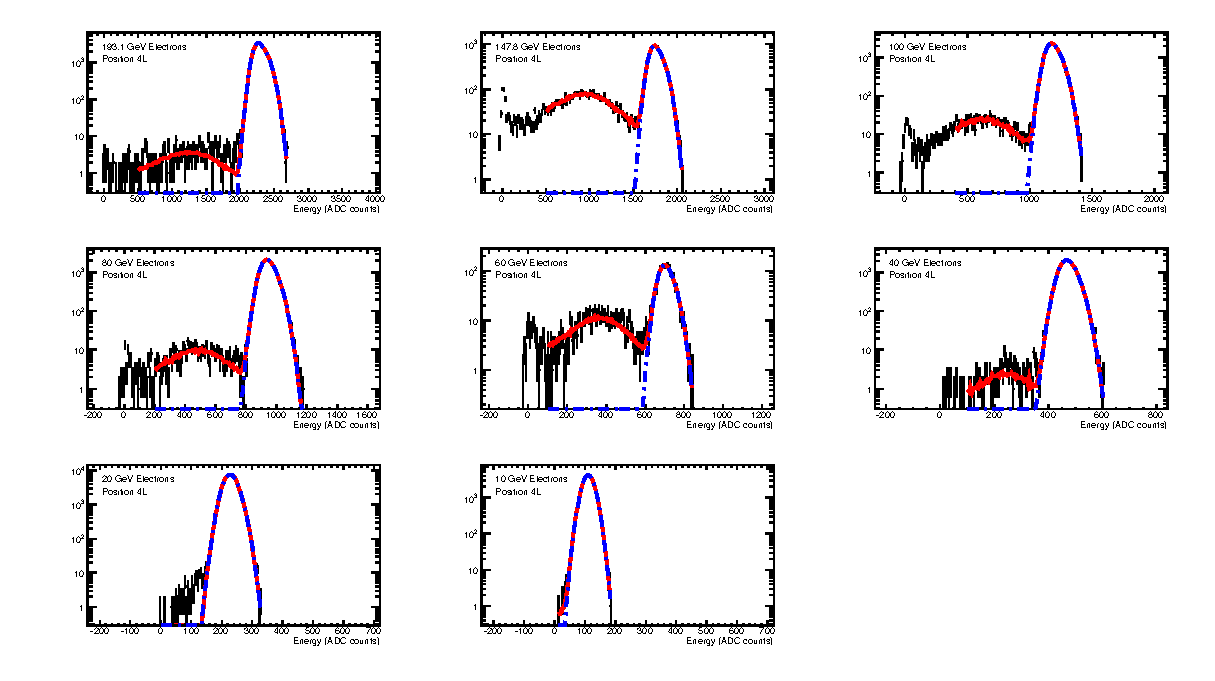
\includegraphics[width=1.0\linewidth,angle=0]{FCalTB_plots/electron_response_4L_data.eps}
%\end{center}
%\caption{Response of the FCal to electron beams at position 4L. The blue dashed curve double Gaussian fit to the electron peak, while the red curve shows the total fit to the electron peak plus the contaminant hadron contribution.}
%\label{TBplot_electron_response_4L_data}
%\end{figure}


The simulated response to electrons is shown in Figure~\ref{TB_electron_MC_response_4L} for position 4L and Figure~\ref{TBplot_electron_response_4H_MC} for position 4H, while the fit results and clustered noise are listed in Tables \ref{TBres_table_elec_4LMC} and \ref{TBres_table_elec_4HMC}. All of the physics lists described in Section~\ref{TB_overview_g4} model electromagnetic showers in the same way, so no distinction between physics lists is made for the simulation results for electrons. 

%noise noise noise.



%%%%%%%%%%%%%%%%%%%%%%%%%%%%%%%%%%%%%%%%%%%%%%%%%%%%%%%%%%%%%%%%
%\begin{figure}[!htb]
%\begin{center}
%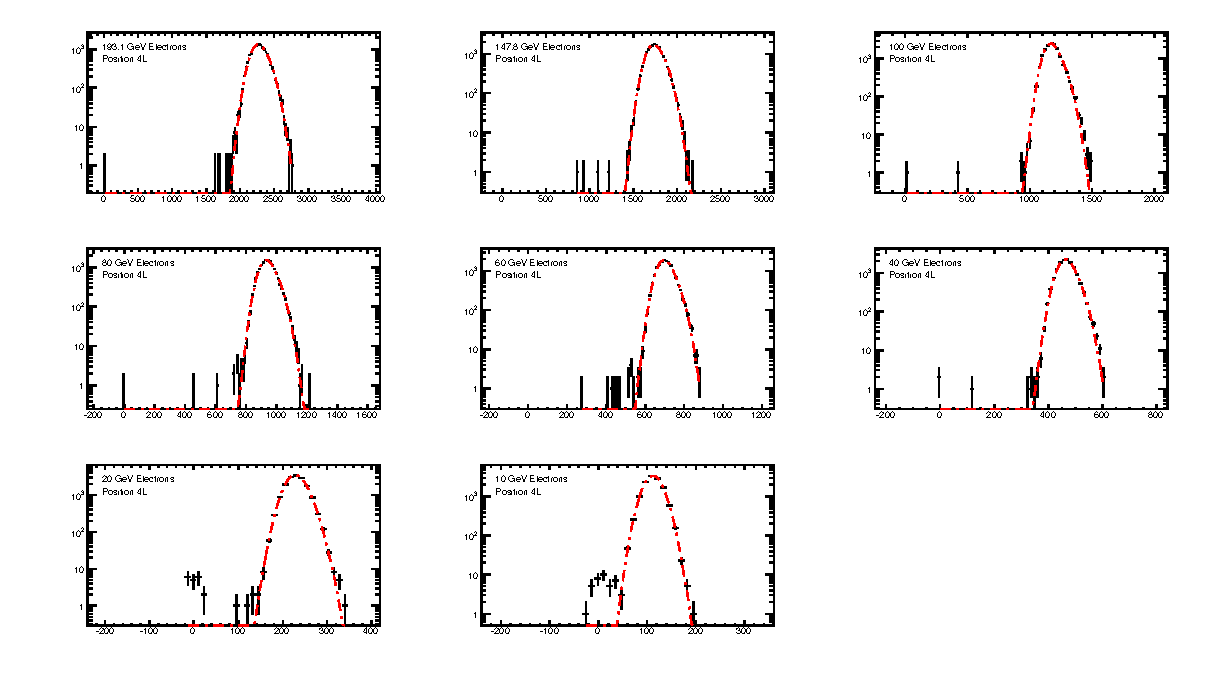
\includegraphics[width=1.0\linewidth,angle=0]{FCalTB_plots/electron_response_4L_MC.eps}
%\end{center}
%\caption{Monte Carlo results for electron beams at position 4L.}
%\label{TBplot_electron_response_4L_MC}
%\end{figure}
%%%%%%%%%%%%%%%%%%%%%%%%%%%%%%%%%%%%%%%%%%%%%%%%%%%%%%%%%%%%%%%%
%%%%%%%%%%%%%%%%%%%%%%%%%%%%%%%%%%%%%%%%%%%%%%%%%%%%%%%%%%%%%%%
\begin{figure}[tbp]
\begin{center}
\subfigure{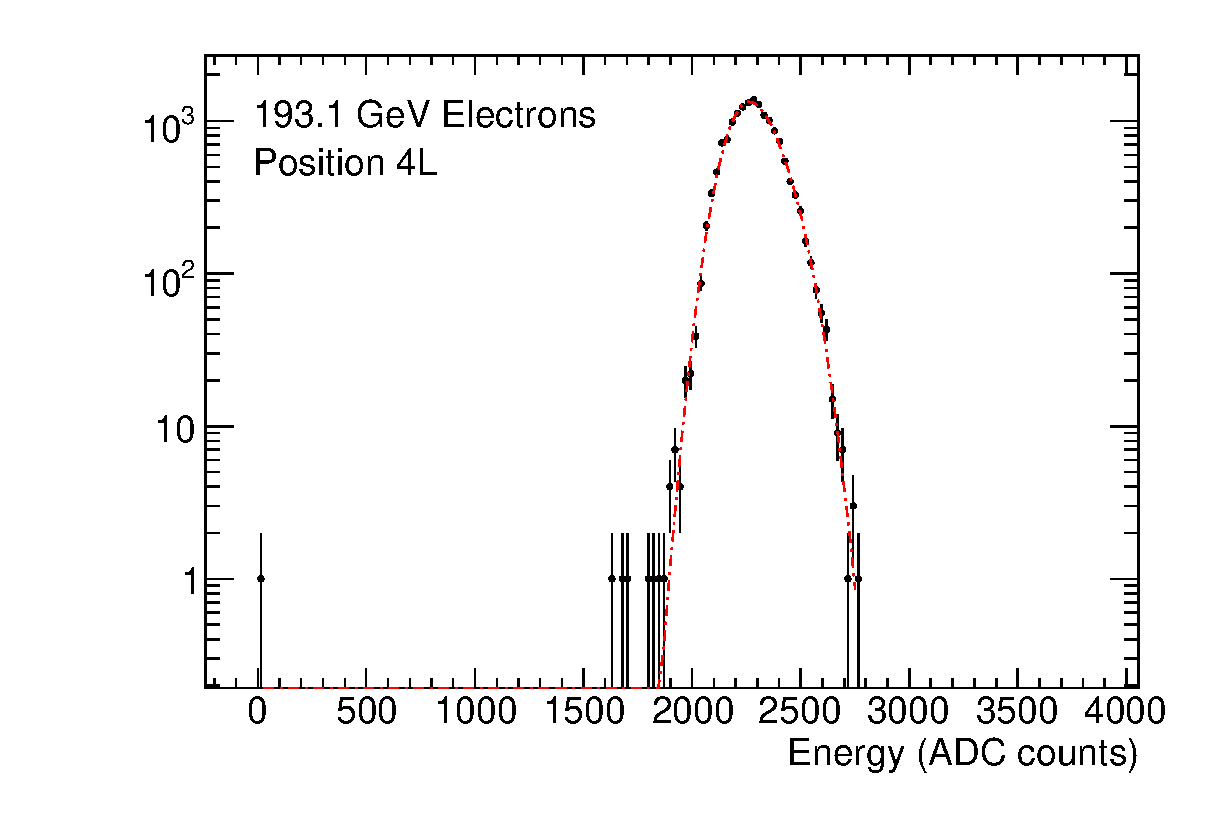
\includegraphics[width=0.45\linewidth,angle=0]{FCalTB_plots/Response_individual_MC/Electron_response_193GeV_4L_MC.eps}}
\subfigure{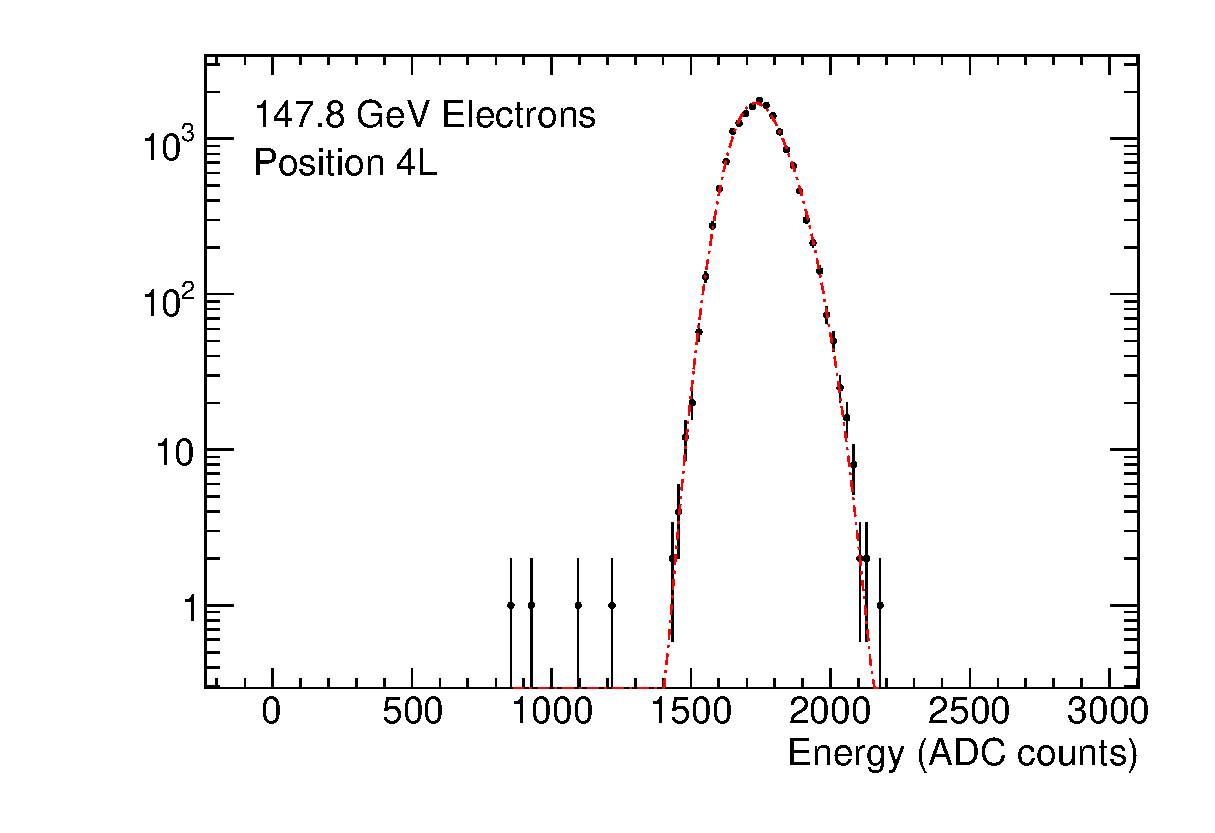
\includegraphics[width=0.45\linewidth,angle=0]{FCalTB_plots/Response_individual_MC/Electron_response_148GeV_4L_MC.eps}}\\
\subfigure{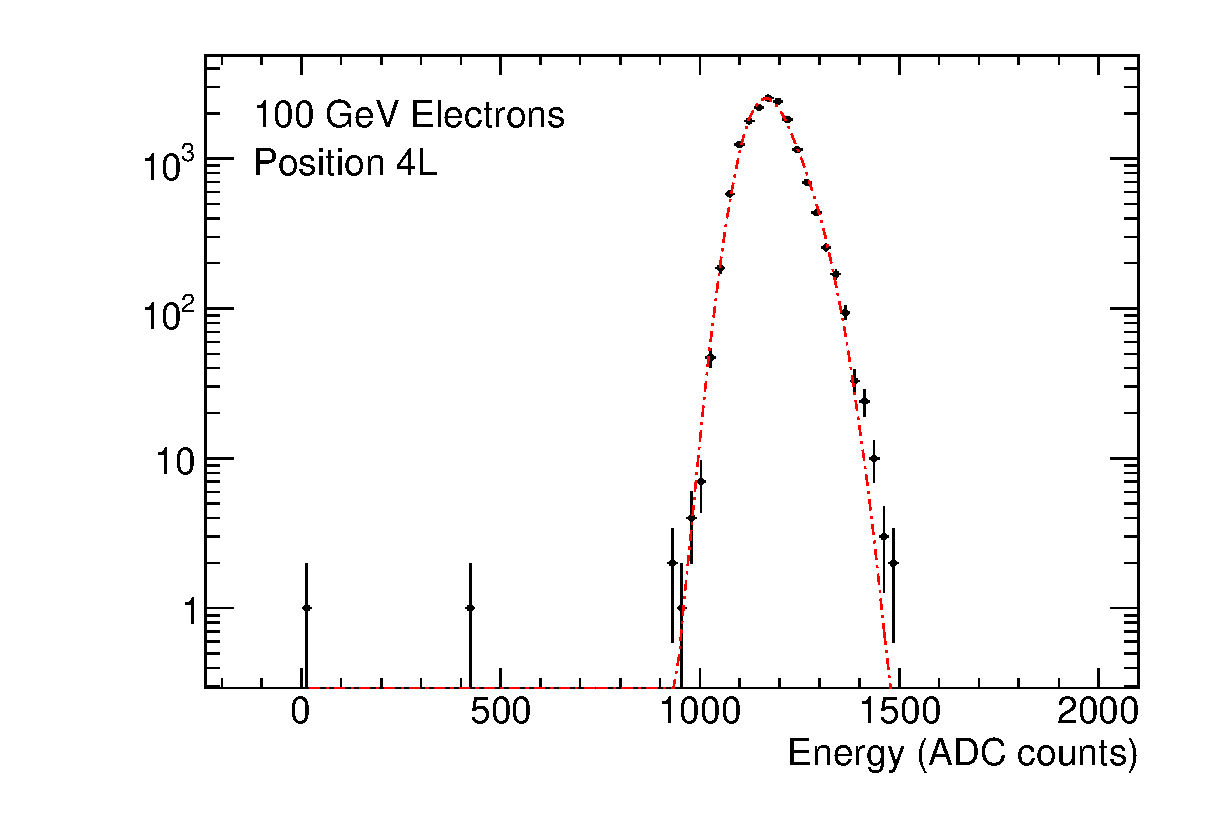
\includegraphics[width=0.45\linewidth,angle=0]{FCalTB_plots/Response_individual_MC/Electron_response_100GeV_4L_MC.eps}}
\subfigure{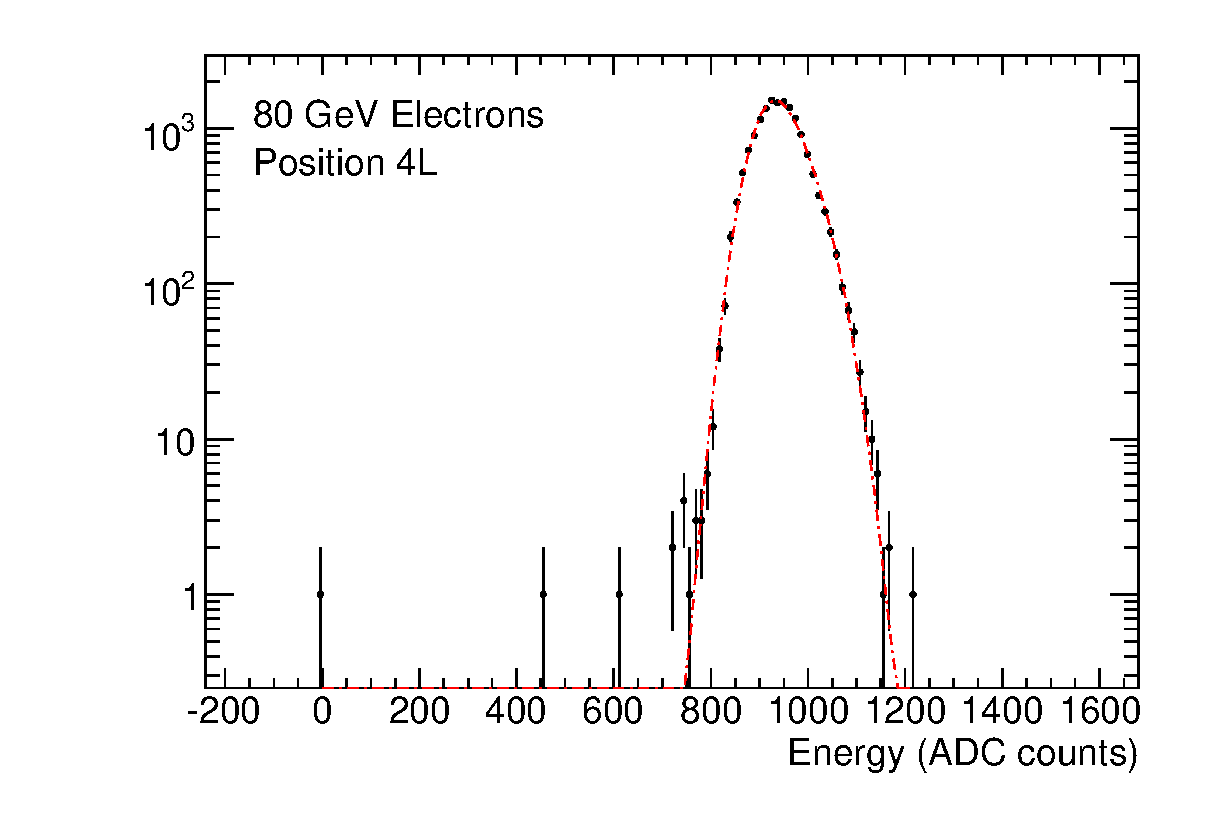
\includegraphics[width=0.45\linewidth,angle=0]{FCalTB_plots/Response_individual_MC/Electron_response_80GeV_4L_MC.eps}}\\
\subfigure{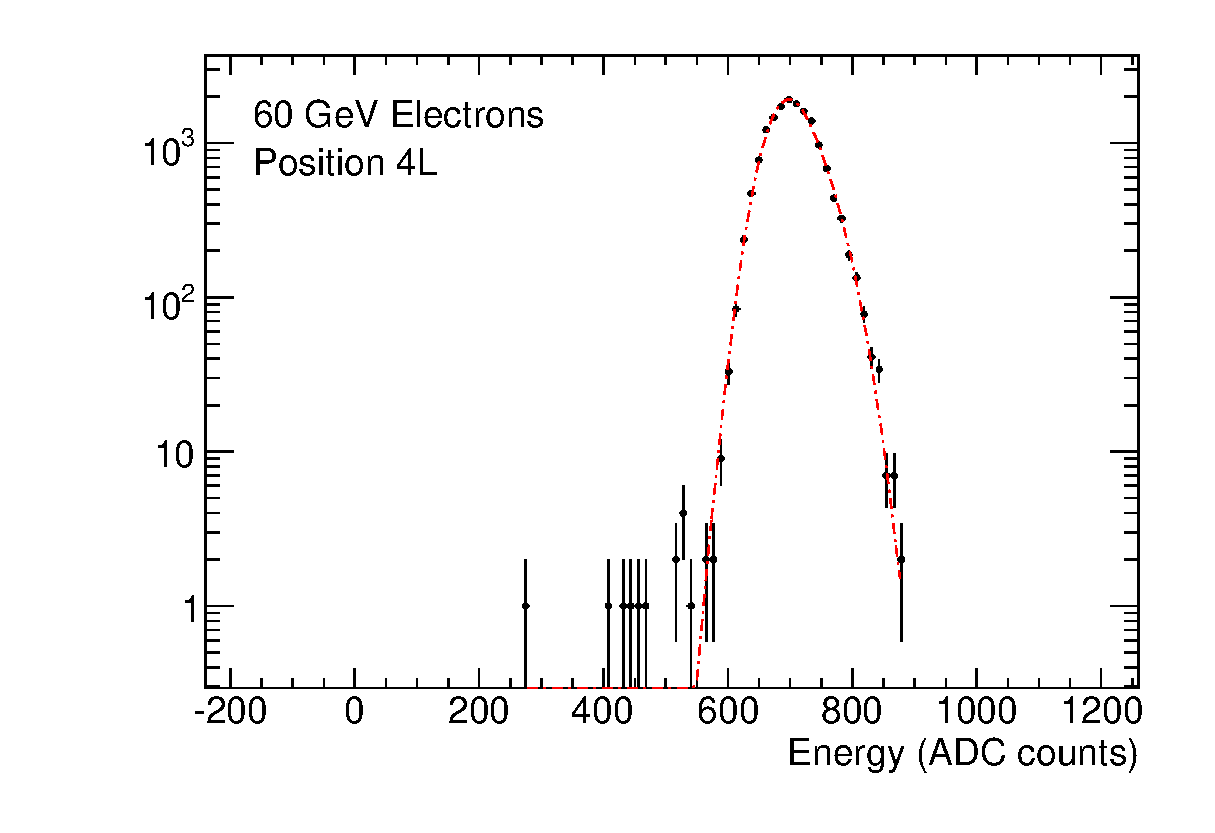
\includegraphics[width=0.45\linewidth,angle=0]{FCalTB_plots/Response_individual_MC/Electron_response_60GeV_4L_MC.eps}}
\subfigure{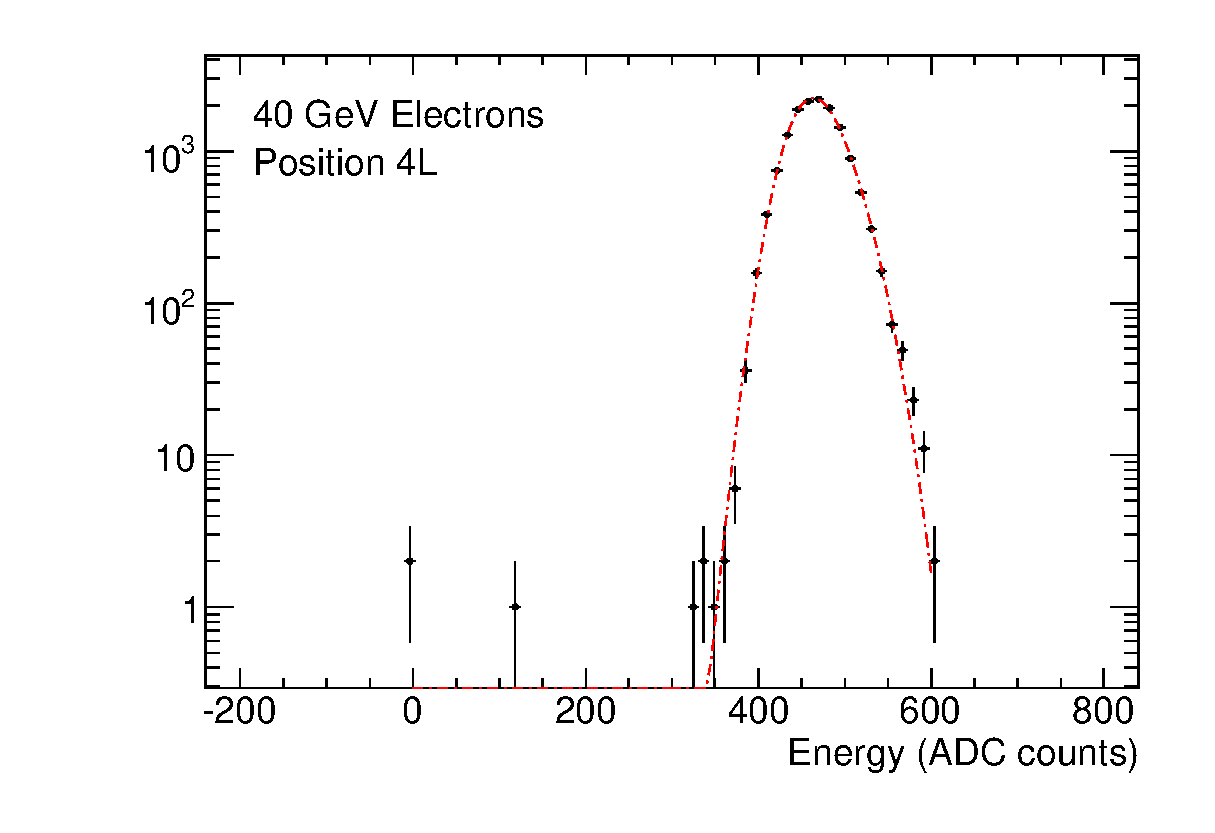
\includegraphics[width=0.45\linewidth,angle=0]{FCalTB_plots/Response_individual_MC/Electron_response_40GeV_4L_MC.eps}}\\
\subfigure{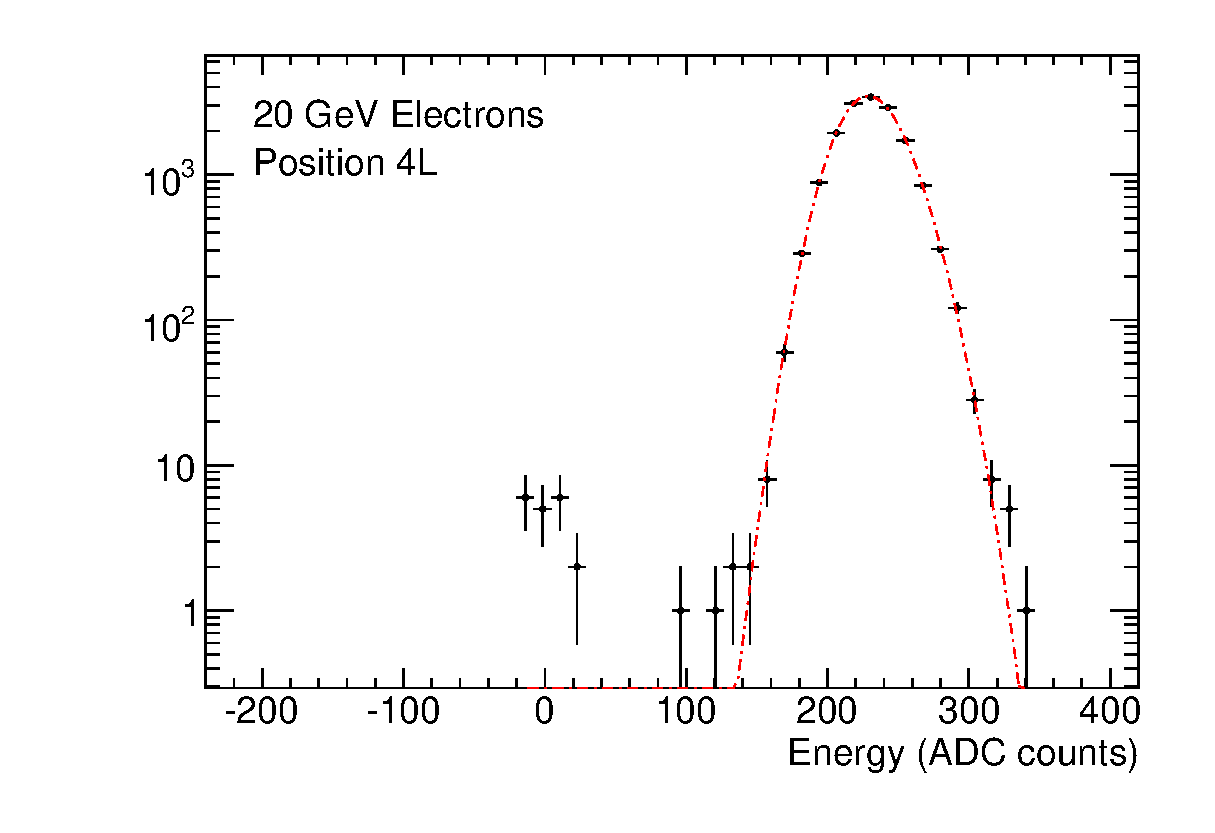
\includegraphics[width=0.45\linewidth,angle=0]{FCalTB_plots/Response_individual_MC/Electron_response_20GeV_4L_MC.eps}}
\subfigure{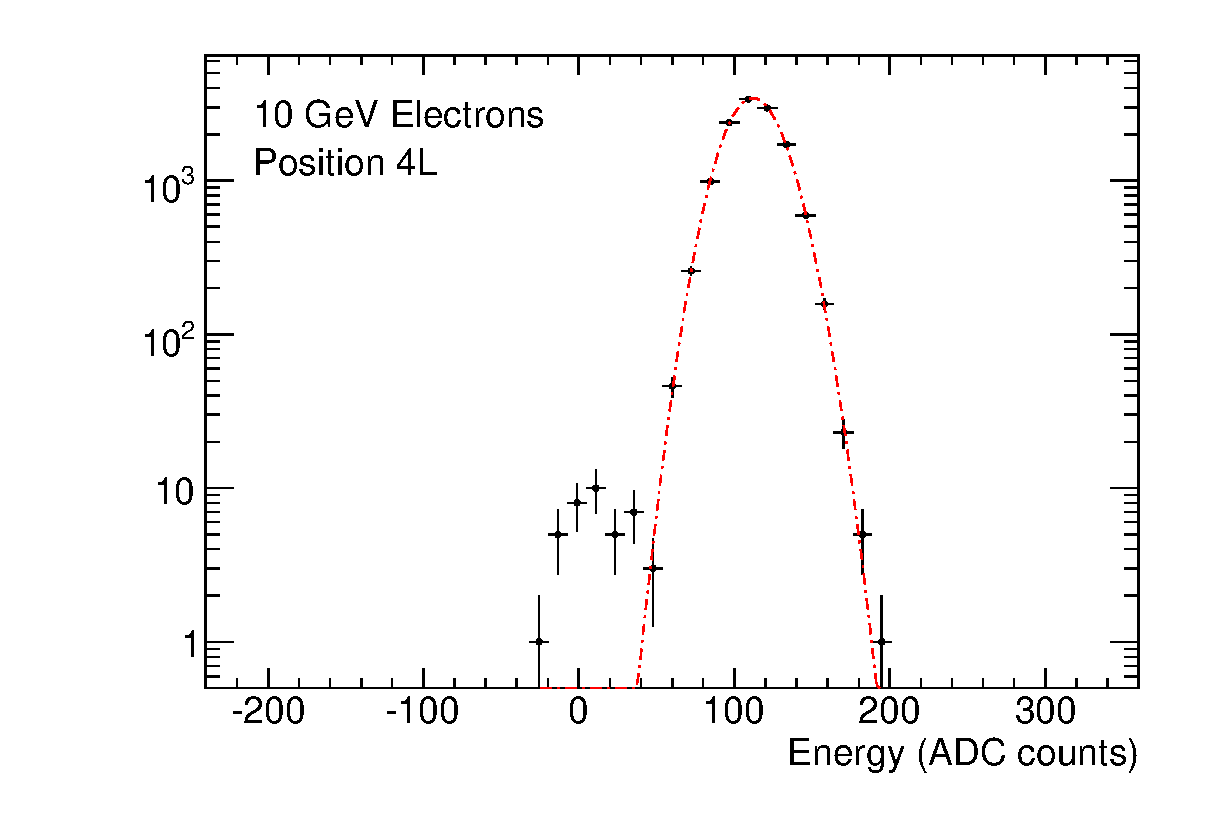
\includegraphics[width=0.45\linewidth,angle=0]{FCalTB_plots/Response_individual_MC/Electron_response_10GeV_4L_MC.eps}}\\
\end{center}
\caption[Monte Carlo results for electrons at position 4L]{Monte Carlo results for electrons at position 4L. The red curve shows the double Gaussian fit to the response.}
\label{TB_electron_MC_response_4L}
\end{figure}

%%%%%%%%%%%%%%%%%%%%%%%%%%%%%%%%%%%%%%%%%%%%%%%%%%%%%%%%%%%%%%%
%maybe some words go here
%%%%%%%%%%%%%%%%%%%%%%%%%%%%%%%%%%%%%%%%%%%%%%%%%%%%%%%%%%%%%%%

\begin{figure}[p]
\begin{center}
\subfigure{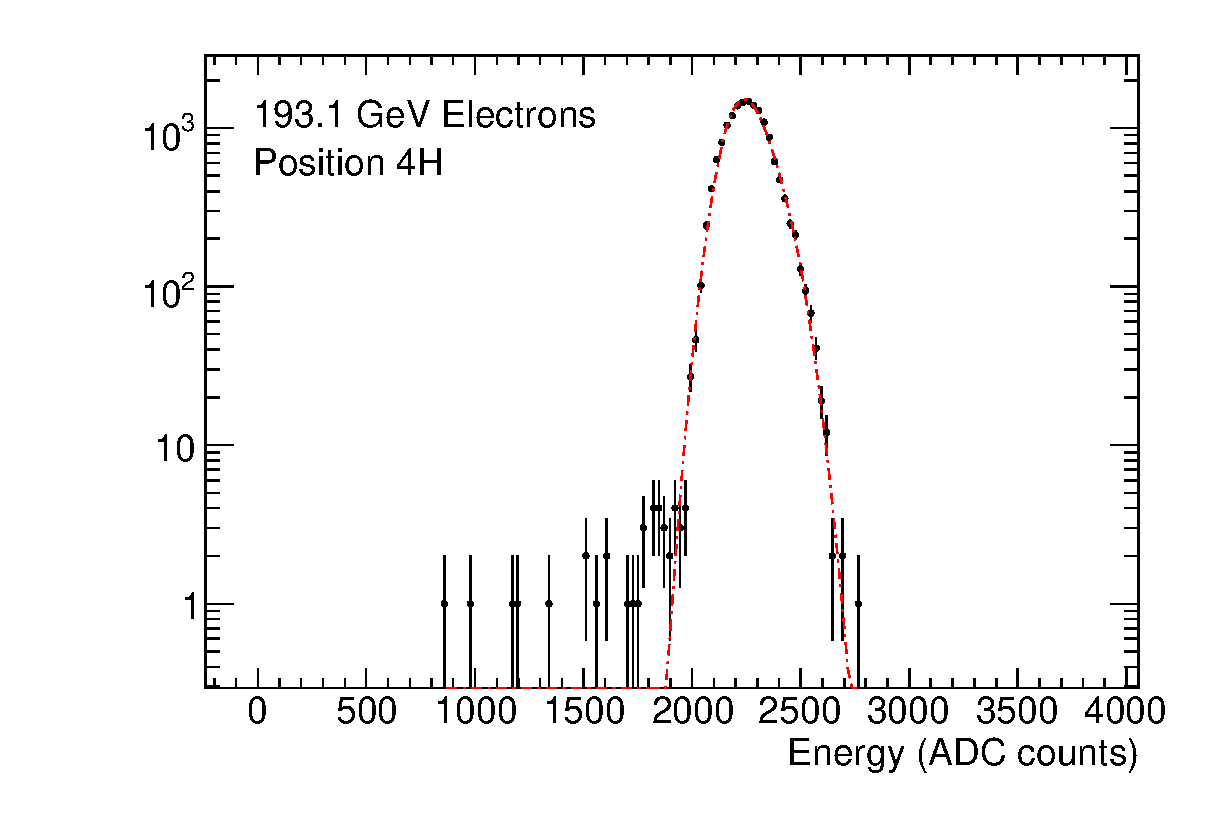
\includegraphics[width=0.45\linewidth,angle=0]{FCalTB_plots/Response_individual_MC/Electron_response_193GeV_4H_MC.eps}}
\subfigure{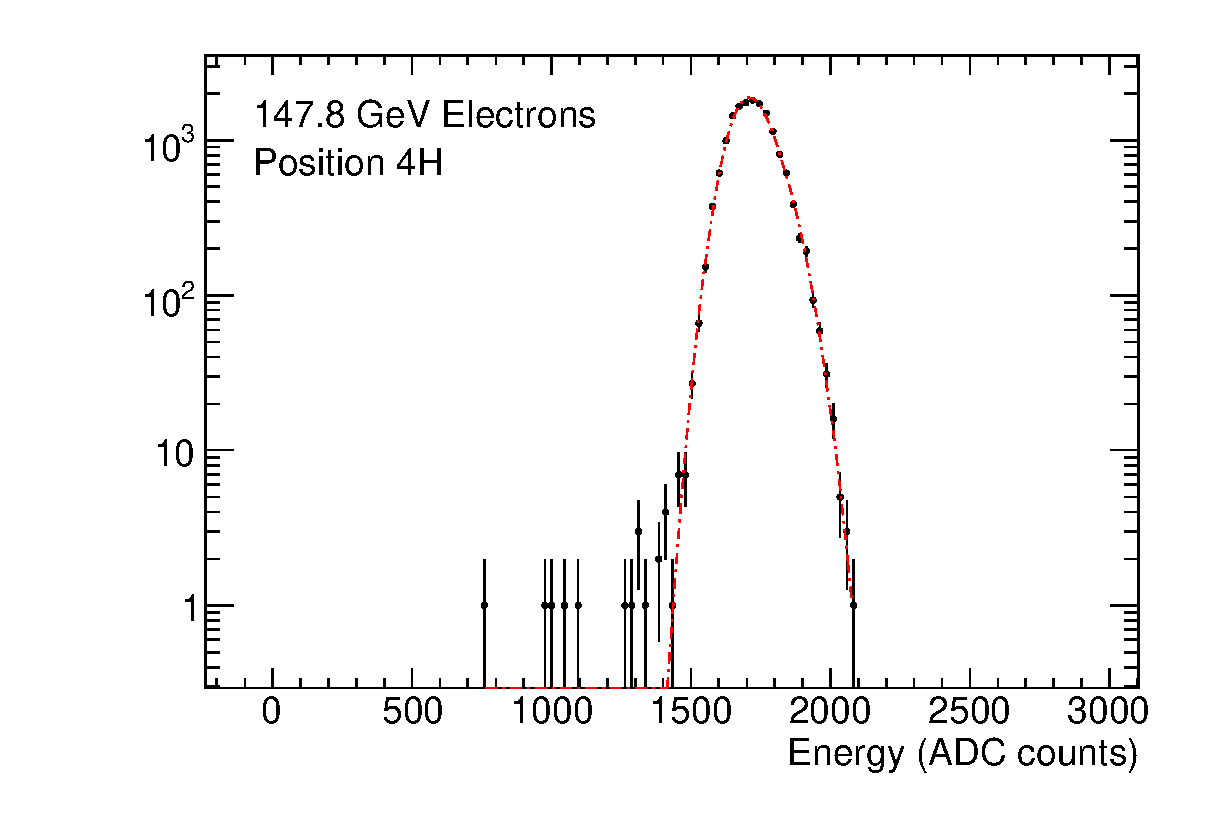
\includegraphics[width=0.45\linewidth,angle=0]{FCalTB_plots/Response_individual_MC/Electron_response_148GeV_4H_MC.eps}}\\
\subfigure{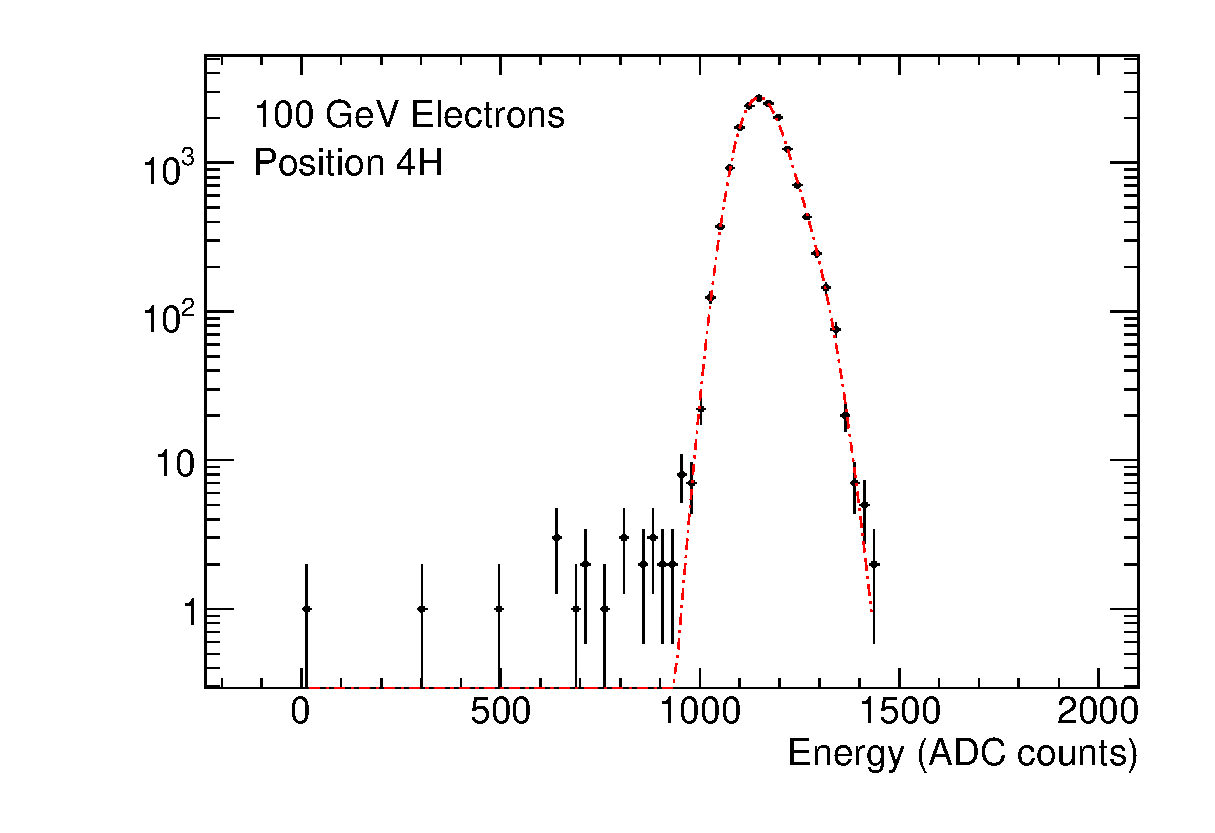
\includegraphics[width=0.45\linewidth,angle=0]{FCalTB_plots/Response_individual_MC/Electron_response_100GeV_4H_MC.eps}}
\subfigure{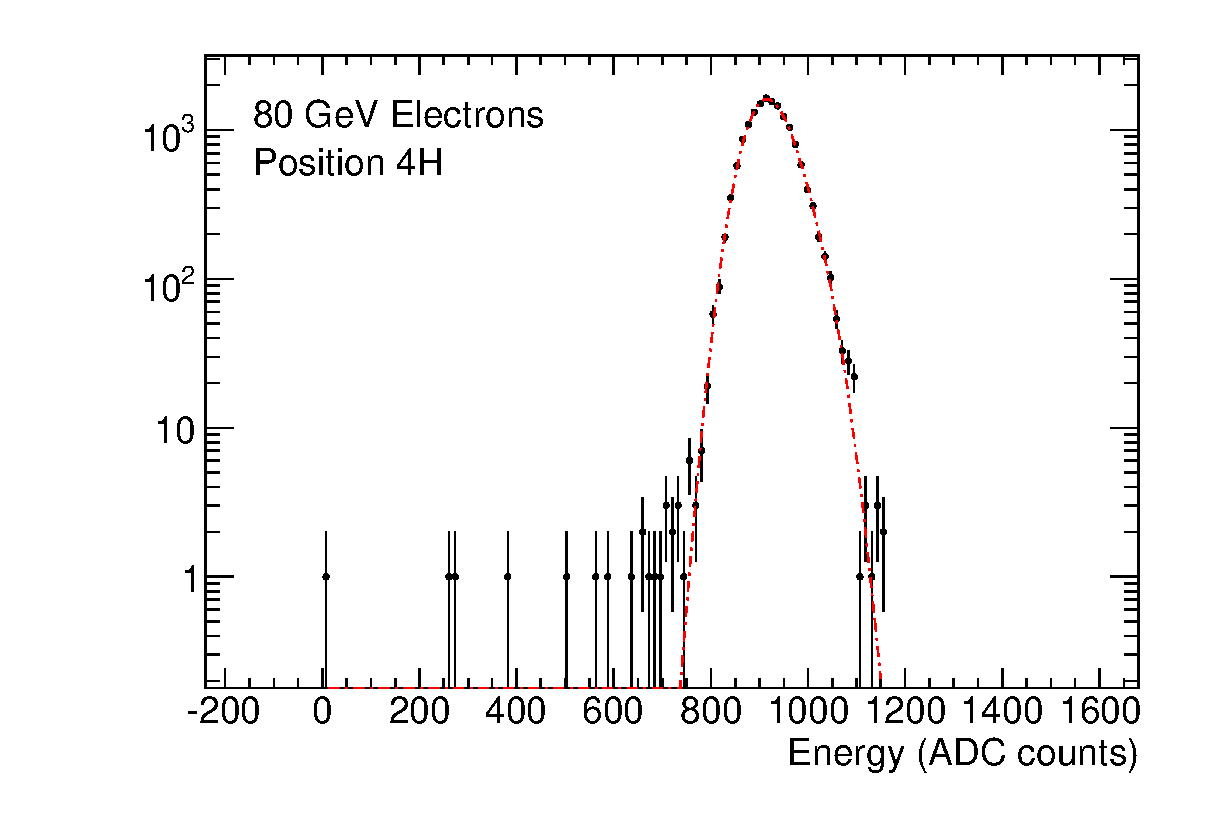
\includegraphics[width=0.45\linewidth,angle=0]{FCalTB_plots/Response_individual_MC/Electron_response_80GeV_4H_MC.eps}}\\
\subfigure{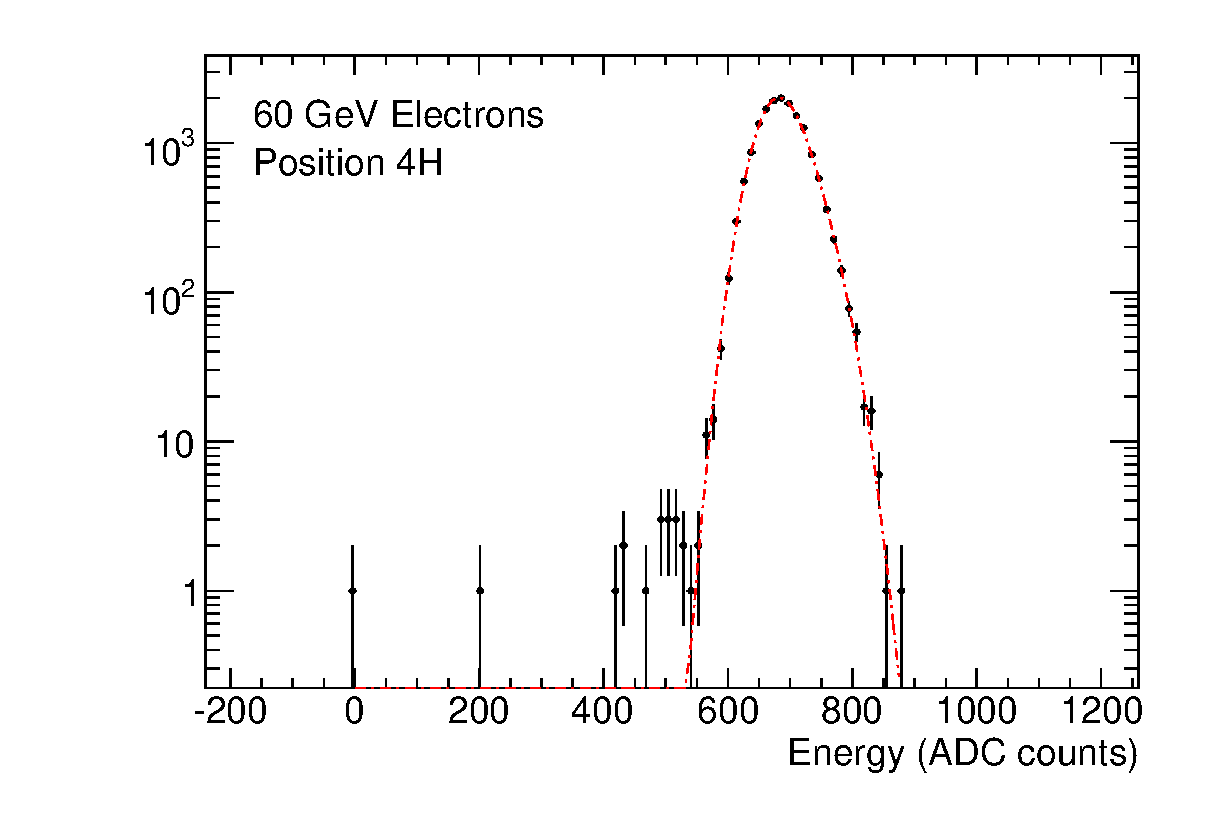
\includegraphics[width=0.45\linewidth,angle=0]{FCalTB_plots/Response_individual_MC/Electron_response_60GeV_4H_MC.eps}}
\subfigure{\includegraphics[width=0.45\linewidth,angle=0]{FCalTB_plots/Response_individual_MC/Electron_response_40GeV_4H_MC.eps}}\\
\subfigure{\includegraphics[width=0.45\linewidth,angle=0]{FCalTB_plots/Response_individual_MC/Electron_response_20GeV_4H_MC.eps}}
\subfigure{\includegraphics[width=0.45\linewidth,angle=0]{FCalTB_plots/Response_individual_MC/Electron_response_10GeV_4H_MC.eps}}\\
\end{center}
\caption[Monte Carlo results for electrons at position 4H]{Monte Carlo results for electrons at position 4H. The red curve shows the double Gaussian fit to the response.}
\label{TBplot_electron_response_4H_MC}
\end{figure}
%%%%%%%%%%%%%%%%%%%%%%%%%%%%%%%%%%%%%%%%%%%%%%%%%%%%%%%%%%%%%%%


%%%%%%%%%%%%%%%%%%%%%%%%%%%%%%%%%%%%%%%%%%%%%%%%%%%%%%%%%%%%%%%
\begin{table}[p]
\begin{center}
\begin{tabular}{|l|l|l|l|}
\hline
Beam Energy (GeV) & Fitted Mean (ADC)& Fitted Width (ADC)& Noise (ADC) \\
\hline
193.1 GeV  &  2285.2 $\pm$     0.9 &   114.3 $\pm$     0.7 &    14.2 $\pm$     0.1 \\
147.8 GeV  &  1747.4 $\pm$     0.7 &    91.3 $\pm$     0.5 &    17.0 $\pm$     0.1 \\
100 GeV  &  1180.2 $\pm$     0.5 &    62.5 $\pm$     0.3 &    17.4 $\pm$     0.1 \\
80 GeV  &   942.8 $\pm$     0.4 &    51.7 $\pm$     0.3 &    14.1 $\pm$     0.1 \\
60 GeV  &   705.3 $\pm$     0.3 &    40.9 $\pm$     0.2 &    14.2 $\pm$     0.1 \\
40 GeV  &   467.9 $\pm$     0.3 &    31.6 $\pm$     0.2 &    14.5 $\pm$     0.1 \\
20 GeV  &   230.5 $\pm$     0.2 &    22.2 $\pm$     0.1 &    14.3 $\pm$     0.1 \\
10 GeV  &   112.5 $\pm$     0.2 &    18.0 $\pm$     0.1 &    14.3 $\pm$     0.1 \\
5 GeV  &    53.1 $\pm$     0.1 &    16.9 $\pm$     0.1 &    14.1 $\pm$     0.1 \\
\hline
\end{tabular}
\end{center}
\caption[Simulated response of the FCal to electron beams at position 4L]{Simulated response of the FCal to electron beams at position 4L. Quoted uncertainties are statistical only.}
\label{TBres_table_elec_4LMC}
\end{table}
%%%%%%%%%%%%%%%%%%%%%%%%%%%%%%%%%%%%%%%%%%%%%%%%%%%%%%%%%%%%%%%

%maybe some words go here




%%%%%%%%%%%%%%%%%%%%%%%%%%%%%%%%%%%%%%%%%%%%%%%%%%%%%%%%%%%%%%%%
%\begin{figure}[!htb]
%\begin{center}
%\includegraphics[width=1.0\linewidth,angle=0]{FCalTB_plots/electron_response_4H_MC.eps}
%\end{center}
%\caption{Monte Carlo results for electron beams at position 4H.}
%\label{TBplot_electron_response_4H_MC}
%\end{figure}
%%%%%%%%%%%%%%%%%%%%%%%%%%%%%%%%%%%%%%%%%%%%%%%%%%%%%%%%%%%%%%%%




%%%%%%%%%%%%%%%%%%%%%%%%%%%%%%%%%%%%%%%%%%%%%%%%%%%%%%%%%%%%%%%
\begin{table}[p]
\begin{center}
\begin{tabular}{|l|l|l|l|}
\hline
Beam Energy (GeV) & Fitted Mean (ADC)& Fitted Width (ADC)& Noise (ADC) \\
\hline
193.1 GeV  &  2259.7 $\pm$     0.8 &   103.2 $\pm$     0.6 &    15.9 $\pm$     0.1 \\
147.8 GeV  &  1723.5 $\pm$     0.7 &    82.8 $\pm$     0.5 &    15.6 $\pm$     0.1 \\
100 GeV  &  1159.5 $\pm$     0.4 &    58.4 $\pm$     0.3 &    17.0 $\pm$     0.1 \\
80 GeV  &   923.0 $\pm$     0.4 &    48.2 $\pm$     0.3 &    17.1 $\pm$     0.1 \\
60 GeV  &   687.7 $\pm$     0.3 &    39.3 $\pm$     0.2 &    16.1 $\pm$     0.1 \\
40 GeV  &   452.4 $\pm$     0.2 &    30.7 $\pm$     0.2 &    15.0 $\pm$     0.1 \\
20 GeV  &   218.8 $\pm$     0.2 &    22.3 $\pm$     0.1 &    14.6 $\pm$     0.1 \\
10 GeV  &   103.5 $\pm$     0.1 &    18.4 $\pm$     0.1 &    14.3 $\pm$     0.1 \\
\hline
\end{tabular}
\end{center}
\caption[Simulated response of the FCal to electron beams at position 4H]{Simulated response of the FCal to electron beams at position 4H. Quoted uncertainties are statistical only.}
\label{TBres_table_elec_4HMC}
\end{table}
%%%%%%%%%%%%%%%%%%%%%%%%%%%%%%%%%%%%%%%%%%%%%%%%%%%%%%%%%%%%%%%

The linearity of the FCal response to electrons is shown in Figures~\ref{TBplot_electron_linearity_4L} (for position 4L) and \ref{TBplot_electron_linearity_4H} (position 4H), depicting the mean reconstructed energy (in ADC counts) as a function of beam energy. In each case the results of a linear fit have been overlaid, the results of which are given in Table \ref{table_electron_c8_linearity}. The $y$ intercept was not fixed to zero when performing the fit. The negative result for the intercept is attributed to energy losses in the upstream material, with the additional material at 4H resulting in an intercept larger in magnitude than that at 4L. As the simulation only modelled beamline components downstream of the B9 magnet, energy losses in materials upstream of this point would not be reflected in the simulation results. This is a possible explanation as to why the simulation results have a less negative intercept than those obtained from data. The effects of the additional material in front of position 4H appear to be well modelled by the simulation, as can be seen by comparing the values of the intercepts at position 4L and 4H. In data, the intercept at 4H is 8.3 ADC counts lower than that measured at position 4L, while in the simulation results there is a difference of 9.0 ADC counts. \cmt{The residuals obtained from the linearity fits are plotted in Figure~\ref{TBplot_electron_residuals}. From the plot in Figure ~\ref{TBplot_electron_residuals_4L}, it can be seen that the response at position 4L is linear to within $1\%$. This is also the case at position 4H for energies of 20~GeV and above.} 


%The two dominant sources of systematic uncertainty on the linearity arise from the cluster radius and the beam polarity. 
One of the larger sources of systematic uncertainty on the response linearity is due to effects related to the beam polarity. The electron beams used in this study were secondary or tertiary beams produced by directing proton beams from the SPS at a fixed target\cmt{lead}. At higher energies a secondary beam was used, the polarity of which ($e^+$ or $e^-$) was determined based on the needs of experiments in the neighbouring H8 beamline. At lower energies a tertiary beam was used, the polarity of which could be chosen freely. %The magnets used in the beamline \red{ were not} systematically de-gaussed between runs at different beam polarities.
%Data taken at 4L with both e+ beams and e- beams is available at two energy points: 10~GeV and 20~GeV

Data was taken at position 4L using both $e^-$ and $e^+$ beams at energies of 10~GeV and 20~GeV. Electromagnetic showers induced by electrons should on average deposit the same energy as those initiated by positrons. The 10~GeV and 20~GeV results in Figure~\ref{TBplot_electron_response_4L_data} combine data obtained from both $e^+$ and $e^-$ beams. When beams of opposite polarity were considered separately, the response to 10~GeV positrons was found to be on average ($1.7 \pm 0.1$)\% higher than the response to electrons. At 20~GeV, the response to positrons was found to be ($1.01 \pm 0.05$) \% higher than the response to electrons. This variation in response is attributed to conditions in the magnet systems. The magnets were not systematically de-Gaussed during data taking, and so it is possible that hysteresis effects may have led to some small variations in the beam energy. These variations in the beam energy are considered as a source of systematic uncertainty.

%minus
%228.027 21.6536 38078.6 227.945 21.4839 38160.2 0.0568748 14.7286 -> 228.027 +/- .08
%109.91 17.7133 17422.4 109.888 17.6825 17358.2 0.040217 14.4115 -> 109.91 +/- .076 (10.095/sqrt(17422.4)) 
%plus
%230.331 21.5863 45655.1 230.254 21.4087 45759.3 -0.0945491 14.401 -> +/- 0.07
%111.776 17.5955 21307.5 111.765 17.6214 21246.8 0.0434593 14.4027-> +/- 0.07

%20 GeV -> 1.0101 +/- .0005
%10 GeV -> 1.0169 +/- .001


% This variation in the response is attributed to variations in the beam conditions. The beam magnets were not systematically de-gaussed, and so .
%
% This difference in response is attributed to variation in the beam conditions, and is considered as a source of systematic uncertainty. 


%e+ 1.6% higher than e- at 10~GeV, 4L
%e+ 1.0% higher than e- at 20~GeV





%%%%%%%%%%%%%%%%%%%%%%%%%%%%%%%%%%%%%%%%%%%%%%%%%%%%%%%%%%%%%%%%
%\begin{figure}[!htb]
%\begin{center}
%\includegraphics[width=0.95\linewidth,angle=0]{FCalTB_plots/electron_linearity_4L.eps}
%\end{center}
%\caption{Linearity of the response to electrons at position 4L. }
%\label{TBplot_electron_linearity_4L}
%\end{figure}
%%%%%%%%%%%%%%%%%%%%%%%%%%%%%%%%%%%%%%%%%%%%%%%%%%%%%%%%%%%%%%%%
%%%%%%%%%%%%%%%%%%%%%%%%%%%%%%%%%%%%%%%%%%%%%%%%%%%%%%%%%%%%%%%%
%\begin{figure}[!htb]
%\begin{center}
%\includegraphics[width=0.95\linewidth,angle=0]{FCalTB_plots/electron_linearity_4H.eps}
%\end{center}
%\caption{Linearity of the response to electrons at position 4H. }
%\label{TBplot_electron_linearity_4H}
%\end{figure}
%%%%%%%%%%%%%%%%%%%%%%%%%%%%%%%%%%%%%%%%%%%%%%%%%%%%%%%%%%%%%%%%
%%%%%%%%%%%%%%%%%%%%%%%%%%%%%%%%%%%%%%%%%%%%%%%%%%%%%%%%%%%%%%%
\begin{figure}[tb]
\begin{center}
\subfigure[]{\includegraphics[width=0.45\linewidth,angle=0]{FCalTB_plots/electron_linearity_4L.eps}
\label{TBplot_electron_linearity_4L}}
\subfigure[]{
\includegraphics[width=0.45\linewidth,angle=0]{FCalTB_plots/electron_linearity_4H.eps}
\label{TBplot_electron_linearity_4H}
}
\caption[Electron linearity]{Linearity of the response to electrons at position 4L (a) and 4H (b). }
\end{center}
\label{TBplot_electron_linearity}
\end{figure}
%%%%%%%%%%%%%%%%%%%%%%%%%%%%%%%%%%%%%%%%%%%%%%%%%%%%%%%%%%%%%%%
%%%%%%%%%%%%%%%%%%%%%%%%%%%%%%%%%%%%%%%%%%%%%%%%%%%%%%%%%%%%%%%
\begin{figure}[tb]
\begin{center}
\subfigure[]{\includegraphics[width=0.45\linewidth,angle=0]{FCalTB_plots/electron_linearity_residuals_4L_scale.eps}
\label{TBplot_electron_residuals_4L}}
\subfigure[]{\includegraphics[width=0.45\linewidth,angle=0]{FCalTB_plots/electron_linearity_residuals_4H_scale.eps}
\label{TBplot_electron_residuals_4H}}
\end{center}
\caption[Electron linearity residuals]{Residuals obtained from the linearity fit for electrons at position 4L (a) and 4H (b). Solid lines in the error bars represent the statistical uncertainties, while the systematic uncertainties are represented by dotted lines. }
\label{TBplot_electron_residuals}
\end{figure}
%%%%%%%%%%%%%%%%%%%%%%%%%%%%%%%%%%%%%%%%%%%%%%%%%%%%%%%%%%%%%%%

%%%%%%%%%%%%%%%%%%%%%%%%%%%%%%%%%%%%%%%%%%%%%%%%%%%%%%%%%%%%%%%
\begin{table}[htb]
\begin{center}
\begin{tabular}{|l|l|l|l|}
\hline
linearity result & slope (ADC/GeV)& Intercept (ADC) \\
\hline
Data (4L) & 11.966 $\pm$ 0.002 & -9.26 $\pm$ 0.07 \\
Simulation (4L) & 11.865 $\pm$ 0.003 & -6.45 $\pm$ 0.13 \\
Data (4H) & 11.693 $\pm$ 0.002 & -17.53 $\pm$ 0.10 \\
Simulation (4H) & 11.747 $\pm$ 0.003 & -15.44 $\pm$ 0.13 \\
\hline
\end{tabular}
\caption[Electron linearity results]{Linearity results for electron data. Quoted uncertainties are statistical.}
\label{table_electron_c8_linearity}
\end{center}
\end{table}



%\blue{
%The linearity of the FCal response shown in Figure~\ref{TBplot_electron_linearity_4L} uses events from both $e^+$ and $e^-$ runs at energies of 10~GeV and 20~GeV. which is considered to be the "nominal" case At each of each of these energies, the response may be determined using events from $e+$ runs, events from $e-$ runs, or events from either $e^+$ or $e^-$ runs. A fit to the linearity is performed for each of these cases, and compared to the nominal result. The largest difference observed for each parameter is taken as the systematic uncertainty due to beam polarity effects.


For the 10~GeV and 20~GeV data points in Figure~\ref{TBplot_electron_linearity_4L}, events from both $e^+$ and $e^-$ beams are used. The linear fit obtained in this case is considered the ``nominal'' result. The systematic uncertainty on the linearity due to variations in the beam energy was obtained by varying the data used at 10~GeV and 20~GeV, i.e. using events from only $e^+$ or only $e^-$ runs at each energy. For each of these cases, the linear fit was repeated, and the fit result was compared to the nominal case. The largest difference observed for each parameter has been taken as the systematic uncertainty due to variations in the beam energy.
 
 At position 4H only a single beam polarity was used at each energy, with $e^+$ beams being used at 10~GeV and 20~GeV. The response to $e^-$ beams at 4H was estimated by calculating the ratio of the $e^+$ to $e^-$ responses at position 4L, and then scaling the response to $e^+$ beams at 4H by this ratio. After obtaining estimates of the response to $e^-$ beams, the uncertainty associated with variations in the beam energy was determined using the same procedure as was done for position 4L.

%To obtain the uncertainty associated with variations in the beam energy, the responses at these points were scaled by the \cmt{$e^+$:$e^-$} ratio of the electron to positron response measured at 4L, in order to estimate the response to $e^-$ beams. 
%
%
%With these estimates of the response to $e^-$ beams at 10GeV and 20GeV, the procedure used at position 4L was repeated in order to obtain the systematic uncertainty on the linearity at position 4H due to fluctuations of the beam energy.


% This yielded four different response combinations, which were then used to estimate the systematic uncertainty.
%}
%%% A fit to the linearity is performed using each response at each energy, giving nine different fit results corresponding to the nine different response combinations. The linearity shown in Figure~\ref{TBplot_electron_linearity_4L} uses events from both $e+$ and $e-$ runs at 10~GeV and 20~GeV, which is considered to be the "nominal" case. For each of the other eight cases, the slope and intercept from the linearity fit are compared to the nominal result, and the largest difference observed for each parameter is taken as the systematic uncertainty due to beam polarity effects. At position 4H, only a single beam polarity was used at each energy, with $e+$ beams being used at 10~GeV and 20~GeV. To obtain the uncertainty due to beam effects the responses at these points was scaled by the $e+$:$e-$ response ratio observed at 4L, in order to estimate the response to $e-$ beams. This yielded four different response combinations, which were then used to estimate the systematic uncertainty.

%As mentioned above, a larger clustering radius captures a slightly larger fraction of the showering particle's energy. However, this also significantly increases the amount of noise present in the cluster, as the noise contribution scales with the number of cells in the cluster. The choice of clustering radius is thus taken as a source of systematic uncertainty on the linearity of the FCal response. This uncertainty was estimated by calculating the linearity of the response using both 12cm and 16cm clusters. The slope obtained using these larger clusters was then compared to the slope obtained using 8cm clusters, with the largest difference being taken as the systematic uncertainty on the slope. The systematic uncertainty on the intercept was obtained the same way.

Other systematic effects considered include the binning used in histograms, whether or not the pion response is included in the electron fit, the signal parameterisation used for the fit, and the event selection criteria. These effects were all found to be small, while the beam energy variations were the most significant source of systematic uncertainty. Systematic uncertainties from different sources were summed in quadrature in order to obtain the final uncertainty on the results. 

%
%\red{fix this}
%Other sources of systematic uncertainty were treated in a similar fashion. For example, the effect of the cluster radius was estimated by using 12cm and 16cm clusters. A fit was performed on the resulting linearity plots, and the fit parameters were compared to those obtained using 8 cm clusters, with the largest difference taken as the uncertainty on that parameter. Systematic uncertainties from different sources were then summed in quadrature to obtain the final uncertainty on the results. 

%At position 4L, the linearity is described by a straight line with slope XX $\pm$ YY and intercept ZZ$\pm$ AA, where the quoted uncertainties are systematic.  

%%With systematic uncertainties taken into account, 


%\blue{deal with the following two paragraphs!}\red{ put results in form XX pm YY (stat) pm YY (sys)}
The linearity at position 4L is best described by a line with slope $11.97 \pm 0.06$  ADC/GeV and intercept -9.3 $\pm$ 1.1 ADC counts, where the quoted uncertainties are dominated by  systematic effects. The statistical uncertainties are given in Table~\ref{table_electron_c8_linearity}. At position 4H, the linearity is described by a line with slope 11.69 $\pm$ 0.06 ADC/GeV and intercept -17.5 $\pm$ 1.3 ADC counts, where the uncertainties are again dominated by systematic effects.

Previous studies of the FCal pulse shapes \cite{Rutherfoord:968060,Rutherfoord:970622} and a SPICE simulation of the FCal electronics chain enabled a prediction of the ADC2GeV calibration factor to be made prior to the beam test. This initial prediction agreed to within 5\% of the value measured at position 4L. However, some impedance mis-matches that had not been accounted for were subsequently identified by analysing pulse shapes recorded when taking  data\cite{Fcalpaper}. These . When the simulation was modified to include these effects, the predicted value of the calibration factor became 12.0 ADC/GeV, improving the agreement with the results presented here.


% A prediction of the ADC2GeV calibration factor was made prior to the beam test, based on a simulation of the FCal electronics chain and knowledge of the FCal structure.
% 
% prediction based on spice simulation of electronics
% 
% electrical properties of electrodes (capacitance, etc)
% 
% drift time of electrons in LAr gaps
% 
% 
% 
% 
%  The predicted value for FCal1 was found to be 12.0 ADC/GeV \cite{Fcalpaper}, in good agreement with the results obtained here.



The residuals obtained from the linearity fits are plotted in Figure~\ref{TBplot_electron_residuals}. From the plot in Figure ~\ref{TBplot_electron_residuals_4L}, it can be seen that the response at position 4L is linear to within $1\%$. This is also the case at position 4H for energies of 20~GeV and above.  Some of the residuals in these figures are still not consistent with zero after including the systematic effects discussed above. It is therefore possible that an unidentified source of systematic uncertainty may contribute at the $\sim$0.5\% level, though this has not been included in the quoted results.

%Systematic uncertainties on the residuals were estimated using the method described above. When performing a fit on the data, the difference between the resulting set of residuals and the nominal residuals is taken as the uncertainty on the residuals due to that particular source of systematic error. The uncertainties from different sources are then summed in quadrature. 
%From the plot in Figure ~\ref{TBplot_electron_residuals_4L}, it can be seen that the response at position 4L is linear to within $1\%$. This is also the case at position 4H for energies of 20~GeV and above.
%% \cmt{something more about the 10~GeV point. Systematics on this point are over 1\%}
%%blahblah
%
%%\clearpage



%%%%%%%%%%%%%%%%%%%%%%%%%%%%%%%%%%%%%%%%%%%%%%%%%%%%%%%%%%%%%%%%
%\begin{figure}[!htb]
%\begin{center}
%\includegraphics[width=0.95\linewidth,angle=0]{FCalTB_plots/electron_residuals_4H_data.eps}
%\end{center}
%\caption{Residuals obtained from the linearity fit for electrons at position 4H. Solid lines in the error bars represent the statistical uncertainties, while the systematic uncertainties are represented by dotted lines. }
%\label{TBplot_electron_residuals_4H}
%\end{figure}
%%%%%%%%%%%%%%%%%%%%%%%%%%%%%%%%%%%%%%%%%%%%%%%%%%%%%%%%%%%%%%%%
%
%%%%%%%%%%%%%%%%%%%%%%%%%%%%%%%%%%%%%%%%%%%%%%%%%%%%%%%%%%%%%%%%
%\begin{figure}[!htb]
%\begin{center}
%\includegraphics[width=0.95\linewidth,angle=0]{FCalTB_plots/electron_residuals_4L_data.eps}
%\end{center}
%\caption{Residuals obtained from the linearity fit for electrons at position 4L. Solid lines in the error bars represent the statistical uncertainties, while the systematic uncertainties are represented by dotted lines. }
%\label{TBplot_electron_residuals_4L}
%\end{figure}
%%%%%%%%%%%%%%%%%%%%%%%%%%%%%%%%%%%%%%%%%%%%%%%%%%%%%%%%%%%%%%%%
%%%%%%%%%%%%%%%%%%%%%%%%%%%%%%%%%%%%%%%%%%%%%%%%%%%%%%%%%%%%%%%%
%\begin{figure}[tb]
%\begin{center}
%\subfigure[]{\includegraphics[width=0.45\linewidth,angle=0]{FCalTB_plots/electron_residuals_4L_data.eps}
%\label{TBplot_electron_residuals_4L}}
%\subfigure[]{\includegraphics[width=0.45\linewidth,angle=0]{FCalTB_plots/electron_residuals_4H_data.eps}
%\label{TBplot_electron_residuals_4H}}
%\end{center}
%\caption{Residuals obtained from the linearity fit for electrons at position 4L (left) and 4H (right). Solid lines in the error bars represent the statistical uncertainties, while the systematic uncertainties are represented by dotted lines. }
%\label{TBplot_electron_residuals}
%\end{figure}
%%%%%%%%%%%%%%%%%%%%%%%%%%%%%%%%%%%%%%%%%%%%%%%%%%%%%%%%%%%%%%%%



The energy resolution of the FCal response to electrons is plotted in Figure~\ref{TBplot_electron_resolution}, for both data and simulation. The randomly triggered events provide information on the amount of noise present in the electronics, and so this information is used to subtract (in quadrature) the noise contribution from the width of the response. This is done because the level of noise was observed to vary over time, such that data collected at different beam energies are affected by different levels of noise. The resolution is thus defined as $\sigma_E/\bar{E}$, where
\begin{equation}
\sigma_E = \sqrt{\sigma^2 - \sigma_N^2}
\end{equation}
where $\sigma_N$ is the width of the noise distribution reconstructed from randomly triggered events. The width of the electron peak, $\sigma$, and the mean response, $\bar{E}$, are obtained from the double Gaussian fit as described by equations~\ref{eqn_moment} and \ref{DG_width_def}. The values of these quantities are listed in in Tables~\ref{TBres_table_elec_4L} and \ref{TBres_table_elec_4H}, for positions 4L and 4H, respectively. As noted earlier, the amount of noise present in the electronics varied over time, but the RMS of the noise contribution to 8 cm clusters was generally around 14-17 ADC counts (1.2-1.4 GeV). The RMS of the noise contribution to the cluster energy has been plotted as a function of beam energy in Figure~\ref{TBplot_noisevbeam_electrons}.


The resolution is fit to a function of the form
\begin{equation}
%\frac{\sigma_E}{E} = \left ( \frac{A^2}{E/GeV} + B^2\right )^{\frac{1}{2}},
\frac{\sigma_E}{\bar{E}} = \frac{A}{\sqrt{E}} \oplus B
\label{resolution_fit_equation}
\end{equation}
which is the same as that given in equation~\ref{eqn_resolution_general} but with the noise term omitted (as the noise contribution to the resolution has been subtracted). The fit results are listed in Table~\ref{table_resolution_electrons}.

%
%\begin{table}[tb]
%\begin{center}
%\begin{tabular}{|l|l|l|l|}
%\hline
%& Stochastic Term (\% $\mathrm{GeV}^{1/2}$) & Constant Term (\%) \\
%\hline
%Data (4L) & 27.0 $\pm$ 0.2 & 3.58 $\pm$ 0.02\\
%Simulation (4L) & 24.7 $\pm$ 0.3 & 4.56 $\pm$ 0.03\\
%Data (4H) & 33.7 $\pm$ 0.2 & 3.11 $\pm$ 0.03\\
%Simulation (4H) & 28.1 $\pm$ 0.3 & 3.96 $\pm$ 0.03\\
%\hline
%\end{tabular}
%\end{center}
%\caption{Fit parameters for energy resolution to electrons. Quoted uncertainties are statistical only.}
%\label{table_resolution_electrons}
%\end{table}


\begin{figure}[tb]
\begin{center}
\subfigure[]{\includegraphics[width=0.45\linewidth,angle=0]{FCalTB_plots/electron_resolution_4L.eps}
\label{TBplot_electron_resolution_4L}}
\subfigure[]{\includegraphics[width=0.45\linewidth,angle=0]{FCalTB_plots/electron_resolution_4H.eps}
\label{TBplot_electron_resolution_4H}}
\caption[Electron energy resolution]{Energy resolution of the FCal to electrons, using data taken from position 4L (a) and 4H (b). A noise subtraction procedure has been applied, as described in the text.}
\label{TBplot_electron_resolution}
\end{center}
\end{figure}
%%%%%%%%%%%%%%%%%%%%%%%%%%%%%%%%%%%%%%%%%%%%%%%%%%%%%%%%%%%%%%%

%%%%%%%%%%%%%%%%%%%%%%%%%%%%%%%%%%%%%%%%%%%%%%%%%%%%%%%%%%%%%%%
\begin{figure}[tb]
\begin{centering}
\subfigure{
\includegraphics[width=0.45\linewidth,angle=0]{FCalTB_plots/Electron_response_4L_data_noisevbeam.eps}
\label{TBplot_noisevbeam_4L}
}
\subfigure{

\includegraphics[width=0.45\linewidth,angle=0]{FCalTB_plots/Electron_response_4H_data_noisevbeam.eps}
\label{TBplot_noisevbeam_4H}
}
\caption[Noise contribution vs beam energy, electrons]{RMS of the electronics noise clustered at different energies, for electron beams at position 4L (a) and position 4H (b).  } 
\label{TBplot_noisevbeam_electrons}
\end{centering}
\end{figure}

%%%%%%%%%%%%%%%%%%%%%%%%%%%%%%%%%%%%%%%%%%%%%%%%%%%%%%%%%%%%%%%


\begin{table}[tb]
\begin{center}
\begin{tabular}{|l|l|l|l|}
\hline
& Stochastic Term (\% $\mathrm{GeV}^{1/2}$) & Constant Term (\%) \\
\hline
Data (4L) & 27.0 $\pm$ 0.2 & 3.58 $\pm$ 0.02\\
Simulation (4L) & 24.7 $\pm$ 0.3 & 4.56 $\pm$ 0.03\\
Data (4H) & 33.7 $\pm$ 0.2 & 3.11 $\pm$ 0.03\\
Simulation (4H) & 28.1 $\pm$ 0.3 & 3.96 $\pm$ 0.03\\
\hline
\end{tabular}
\end{center}
\caption[Electron resolution results]{Fit parameters for energy resolution to electrons. Quoted uncertainties are statistical only.}
\label{table_resolution_electrons}
\end{table}


%The non-uniformity of the response with respect to the beam particle impact point on the calorimeter forms the dominant contribution to the constant term in the resolution 
%The constant term in the electron energy resolution is dominated by the impact point dependence of the response
%
The constant term of the electron energy resolution is influenced by the impact point dependence of the response~\cite{TB95_prototype}. The additional upstream material present for data taken at position 4H can cause the beam particles to begin showering earlier. In such cases, the energy in the shower is then distributed over a larger area by the time it reaches the FCal, decreasing the impact point dependence and resulting in a lower constant term for the resolution measured at position 4H. This effect is seen in both the data and simulation results. 

The simulation results for electrons give a higher (i.e. worse) resolution than that seen in data at higher beam energies, although the discrepancy is smaller at position 4H than 4L. Again, the effects of the additional material at position 4H are well modelled by the simulation. The constant term at position 4L is 15\% higher than that seen at 4H, in both data and simulation, indicating that the effects of the additional material at position 4H are well modelled by the simulation.

%Hokay
%
%simulation results for electron resolution at 4L, 200GeV worse than that seen in data
%
%This has been true for some time now, seen in 98 paper and in TB2004 results. In all cases, electron resolution at 200GeV is around 5\% in simulation but 4\% in data.


The constant term for the resolution is significantly higher in the simulation than in data. This discrepancy is also present in comparisons between \geant simulations and data taken during the 1998 and 2004 testbeams~\cite{TB98_electron_signals,TB2004pub}, with the constant term for the electron resolution obtained from simulations being consistently higher than that seen in data. 

%decided to investigate impact point dependence in data vs MC
%to what degree impact point dependence differs between data and MC
%how much this difference affects the resolution at 200 GeV



%%%%%%%%%%%%%%%%%%%%%%%%%%%%%%%%%%%%%%%%%%%%%%%%%%%%%%%%%%%%%%%
\begin{figure}[tb]
\begin{centering}

\includegraphics[width=0.75\linewidth,angle=0]{FCalTB_plots/electrode_response_v_r.eps}
\label{TBplot_noisevbeam_4L}


%\includegraphics[width=0.45\linewidth,angle=0]{FCalTB_plots/Electron_response_4H_data_noisevbeam.eps}

\caption[Electron response vs distance to closest electrode]{Electron response plotted as a function of $r$, for 193 GeV electrons at position 4L. Note that the liquid argon gap is centred at $r$ = 2.5mm. The red squares represent simulation results in which there is no uncertainty in the impact point position, whereas the blue diamonds represent simulation results in which the impact point has been smeared in a manner consistent with the uncertainties present in the data, as discussed in the text. } 
\label{electrode_r}
\end{centering}
\end{figure}

%%%%%%%%%%%%%%%%%%%%%%%%%%%%%%%%%%%%%%%%%%%%%%%%%%%%%%%%%%%%%%%

As mentioned above, the impact point dependence of the response contributes to the constant term of the resolution.\cmt{ Upstream material can cause beam particles to begin showering earlier, and thus mitigate some of the impact point dependence yielding a lower constant term. This is seen in the 4L/4H data results above. The \geant simulation of the testbeam only includes material downstream of the B9 magnet, and so the material upstream of this magnet is not accounted for in the simulation. This material could cause showers to start earlier in data than in simulation, and thus give rise to the lower constant term seen in data.} Figure~\ref{electrode_r} shows the mean response of the FCal as a function of $r$, which is the radial distance from the impact point to the centre of the closest electrode, for 193 GeV electrons at position 4L. For FCal1, the liquid argon gap covers the region 2.375~mm~$< r <$~2.625~mm, and thus the response is higher near this region. Smaller values of $r$ mean that the electron is striking the copper rod located at the centre of the electrode, leading to a lower response. Note that the simulation results show a larger variation with $r$ than is observed in data, indicating that the impact point dependence of the response is stronger in the simulation than in data. 

When analysing data, the impact point is determined from the beam particle track, which is reconstructed from BPC measurements. The uncertainty on the measured impact point associated with the position resolution of the BPCs is 0.26mm in the $x$ and $y$ coordinates. There is also an uncertainty associated with the alignment between the BPC and FCal coordinate systems, which is $\pm$0.12 mm in the $x$ coordinate and $\pm$0.25mm in the $y$ coordinate~\cite{LouiseThesis}. In the simulation, the trajectories of the beam particles and the precise position of the FCal are known exactly. In order to better compare data and simulation results, the blue diamonds in Figure~\ref{electrode_r} represent simulation results in which the impact points have been artificially smeared in a way that is consistent with the uncertainties present in the data. That is, a shift equal to the alignment uncertainty and a random smearing with RMS equal to the track reconstruction uncertainty were applied to the impact points in the simulation results. 

The noise subtracted electron resolution at 193 GeV is (4.05 $\pm$ 0.02)\% in data, whereas the resolution obtained from simulations is (4.97 $\pm$ 0.03)\%, where the quoted uncertainties are statistical only. In order to estimate how much of this discrepancy could be attributed to the greater impact point dependence seen in the simulation, weights were assigned to the simulated events. Simulated events were binned in $r$\footnote{The ``smeared'' value of $r$ was used for this binning}, and the clustered energy was compared to the mean response observed for that bin in data. If the clustered energy for an event was greater than the mean response seen in data, then the event was assigned a weight $w_i$ (where the index $i$ refers to the $r$-bin being considered), otherwise the event was assigned a weight $1/w_i$. The weight $w_i$ was then determined such that the weighted average response for simulation results in the $i$-th bin was equal to the mean response obtained from the same bin in data.  After weighting the simulation events, the resolution was recalculated and found to be (4.86 $\pm$ 0.01\%), which is still significantly higher than the resolution seen in data. The greater impact point dependence seen in the simulation is thus not sufficient to fully account for the higher resolution seen in the simulation results. 

%
%estimate how much of the resolution discrepancy between data and simulation can be attributed to the greater impact point dependence seen in simulation.
%
%The energy resolution for 193 GeV electrons at position 4L is 4.0\% in data, whereas the simulation results \red{check how PK wants this to be said} 
%
%
%
%
%For the data, the BPCs are used to reconstruct the particle track
%
%
%reweighted electrons - mean 2290.52 , width 112.21, noise 14.2
%resolution @ 193 GeV = 4.86\%
%nominal MC resolution @ 193 GeV = 4.96 \%
%
%red squares - nominal MC
%blue diamonds - misaligned + smeared
%
%


%error calculations for resolution values:
%
%193 GeV electrons 4L data
%DGmean DGwidth  SGN     SGmean  SGwidth noiseN noise m  noise width 
%2300.65 94.4115 34111.5 2300.42 88.8702 35704 -0.181874 15.052
%
%noise subtracted width = 93.203909
%error in noise subtracted width = 0.3447726
%resolution = 4.0512%
%abs error in res = 1.5e-4
%res = 4.05 +/- 0.02
%
%
%193 GeV electrons 4L MC - unweighted
%DGmean DGwidth  SGN     SGmean  SGwidth noiseN noise m  noise width 
%2285.2 114.461 15670.7 2277.61 115.145 15587.5 0.229143 14.2422
%noise subtracted width = 113.57148
%error in Wns = 0.655
%resolution = 4.96987%
%res error =  2.87324 e-4
%
%res = 4.97 +/- 0.03
%
%
%reweighted MC 
%mean = 2290.52, width = 112.21, events = 334568
%SG Mean = 2290.02, SG width = 110.273, SG pop = 332328
%noiseN noise m  noise width 15587.5 0.229143 14.2422
%
%noise subtracted width = 111.30249
%WNS error = 0.136753
%resolution = 4.85926%
%resolution error = 5.9841576e-5
%
%res = 4.86 +/- 0.01
%
%WNS_error[i] = sqrt(  (pow(Width[i],2)*pow(sgWidth[i],2)/2/sgEvents[i]) +( pow(NoiseWidth[i],4)/2/NoiseEvents[i]))/WidthNoiseSub[i];
%
%
%ResError[i] = ResNS[i]*sqrt(pow(WNS_error[i]/WidthNoiseSub[i],2) + pow(sgWidth[i],2)/sgEvents[i]/pow(Mean[i],2));

%\red{insert stuff about data/MC resolution and electrode distance here}
%\red{add stuff about cluster size}
%As mentioned above, a larger clustering radius captures a slightly larger fraction of the showering particle's energy. However, this also significantly increases the amount of noise present in the cluster, as the noise contribution scales with the number of cells in the cluster. The choice of clustering radius is thus taken as a source of systematic uncertainty on the linearity of the FCal response. This uncertainty was estimated by calculating the linearity of the response using both 12cm and 16cm clusters. The slope obtained using these larger clusters was then compared to the slope obtained using 8cm clusters, with the largest difference being taken as the systematic uncertainty on the slope. The systematic uncertainty on the intercept was obtained the same way.
The sources of systematic uncertainty considered for the electron energy resolution are the same as those  considered for the response linearity, although the choice of cluster radius is also considered. As mentioned earlier, a larger clustering radius captures a slightly larger fraction of the showering particle's energy. However, this also significantly increases the amount of noise present in the cluster, as the noise contribution scales with the number of cells in the cluster. The choice of clustering radius is thus taken as a source of systematic uncertainty on the energy resolution of the FCal. This uncertainty was estimated by calculating the resolution using both 12cm and 16cm clusters. The stochastic term obtained using these larger clusters was then compared to that obtained using 8cm clusters, with the largest difference being taken as the systematic uncertainty on the stochastic term. The systematic uncertainty on the constant term was obtained in the same way.

The systematic uncertainties are dominated by beam energy variations and the choice of cluster size, with other effects providing a smaller contribution. The resolution at position 4L is best described by a stochastic term of (27.0 $\pm \, 0.9) \% \cdot (\mathrm{GeV})^{1/2}$ and a constant term of (3.58 $\pm \, 0.09) \%$, while the resolution at position 4H is best described by a stochastic term of (33.7 $\pm 0.8) \% \cdot (\mathrm{GeV})^{1/2}$ and a constant term of (3.11 $\pm 0.09) \%$. These uncertainties are again dominated by systematic effects, with the statistical uncertainties being listed in Table~\ref{table_resolution_electrons}.

The resolution at 4L presented here has a stochastic term of (27.0 $\pm \, 0.9) \% \cdot (\mathrm{GeV})^{1/2}$), which is slightly lower than the published result of (28.5 $\pm \, 1.0) \% \cdot (\mathrm{GeV})^{1/2}$)  \cite{Fcalpaper}. This difference is due to the rounding error discussed in Section~\ref{TBoverview_offline}, which has been corrected in these results but was undiscovered at the time of publication. The constant term presented here (3.58 $\pm \, 0.09) \%$ is slightly larger than the published value (3.5$\pm \, 0.1) \%$, but these values are consistent within the uncertainties. 
%The agreement between data and Monte Carlo is generally good, a


%\red{FIXFIXFIXFIXFIX systematics on electron resolution}



\cmt{ DONE WITH ELECTORNS WOOOOOO}


%The response of the FCal to electrons at position 4L is shown in Figure~\ref{TBplot_electron_response_4L_data}. A beam particle that strikes the calorimeter in the centre of an electrode rod, or in the middle of the absorber, will have a produce a smaller response than a particle that impacts close to the liquid argon gap. As the beamspot has a diameter of 65 mm, which is much greater than the spacing between electrodes (7.5 mm in FCal1), the collected data is derived from many different impact points. 



%geometry-impact point dependence
%double Gaussian used - mean and width taken from the fit
%describe moment calculation used for error in width, mean, etc.
%fit and mean given by 
%6 parameter fit used at 200~GeV, ratio of peak means and populations obtained, used when fitting lower energies - skip this
%
%Results - mean/width Table


%systematic errors - discuss here before linearity stuff.
%Polarity effects.
%
%
%linearity plot, and residuals
%
%
%discussion of linearity,  systematic errors
%- 4L slope of 12.0, agrees with the SPICE simulation.
%intercept allowed to vary, in order to account for upstream material losses.
%c.f. MC - indicates that there is some material not modelled in MC (such as upstream of B9)
%
%
%
%effect of systematics estimated by varying stuff, fitting, and obtaining linearity. systematic uncertainty in slope taken as mac deviation of varied data from nominal analysis.,same for intercept. 
%
%
%
%Noise plot - For each event, a randomly triggered event chosen from the same run. The same channels that are clustered in the "physics" event are summed in the randomly triggered event. In this way a distribution of the clustered noise can be built up, 
%
%Resolution plot
%
%Resolution - noise subtraction method
%
%systematics
%
%quote numbers.













%event selection
%-triggering, scintillators, etc
%-beam cleaning/envelope cuts
%-veto counter
%-timing
%-CEDAR

%analysis
%8cm clustering - relate to Moliere radius, XX\% of the energy should be contained (Wigmans)
%response fitting - double Gaussian, impact point dependence
%linearity
%- SPICE predictions of 12.0~GeV/ADC
%- floating intercept - dead material upstream (CEDAR)
%- systematic uncertainties - polarity, clustering
%
%
%comparison between 4L and 4H, data and MC
%
%
%resolution - noise subtraction
%systematics
%
%comparison between 4L and 4H, data and MC
%
%plots - electron response at 4L
%
%
%\clearpage

\subsection{Analysis of Hadron Data}
\label{section_TB_hadron_results}
%event selection
%- same as for electrons, but with beam envelope oriented at pions
%- CEDAR

%do radial/ longitudinal profiles first, EM scale.
%weights, weight derivation

%response, linearity, resolution, etc.

%beams of pi+ and pi-. 
%Event selection for hadrons is the same as that for electrons, although the CEDAR cut is applied for $\pi+$ beams at all energies below 200GeV in order to reduce the amount of proton contamination. \blue{halflings}. 
%\red{NEED TO REFERENCE ADC2MEV STUFF WITH ELECTRONIC CALIBRATION, WHICH GOES IN DETECTOR CHAPTER}
In the analysis of hadron data, the signal from each FCal module is first calibrated to the electromagnetic (EM) scale by applying the ADC2MeV factors.
%, which convert the reconstructed pulse peak (in ADC counts) to the corresponding energy deposited in the calorimeter by an electromagnetic particle (i.e. an electron or photon). For the beam test, 
The values used to reconstruct signals from the FCal are 83.3 MeV/ADC for FCal1, 163.9 MeV/ADC for FCal2 and 185.2 MeV/ADC for  FCal3. These are the same values used in the published analysis\cite{Fcalpaper}, which were originally obtained using the results of a SPICE simulation of the FCal electronics and calculations pertaining to the FCal's geometry and material. As discussed above, the predicted value for FCal1 is in good agreement with the value obtained from the linear fit to the FCal1 response to electrons. During a previous beam test\cite{TB98_electron_signals}, the response to electrons was studied separately for prototypes of the FCal1 and FCal2 modules. The ratio of these responses was measured from this data, and used to validate the predictions for the EM scale factors of the hadronic modules.

%Data taken in a previous beam test \cite{TB98_electron_signals} studied
%
% allowed the ratio of the FCal1 and FCal2 responses to electrons to be studied, and the SPICE results agree with this data to within 5\%.
%\red{fix this}
%\red{CITE THIS}.


%here are the radial profiles and longitudinal profiles, at the EM scale
% %%%%%%%%%%%%%%%%%%%%%%%%%%%%%%%%%%%%%%%%%%%%%%%%%%%%%%%%%%%%%%%
\begin{figure}[!htb]
\begin{center}

\subfigure[]{
\includegraphics[width=0.45\linewidth,angle=0]{FCalTB_plots/pions_4L_radial_int.eps}
\label{pion_radial_4L_int}
}
\subfigure[]{
\includegraphics[width=0.45\linewidth,angle=0]{FCalTB_plots/pions_4H_radial_int.eps}
\label{pion_radial_4H_int}
} \\
%\caption{Energy distribution within the FCal as a function of the transverse distance ($r$) from the projected beam impact point. Figure~\ref{pion_radial_4L_diff} shows the differential energy distribution while Figure~\ref{pion_radial_4L_int} shows the cumulative distribution. }
%\label{TBplot_radial_profiles_4L}
\subfigure[]{
\includegraphics[width=0.45\linewidth,angle=0]{FCalTB_plots/pions_4L_radial_diff.eps}
\label{pion_radial_4L_diff}
}
\subfigure[]{
\includegraphics[width=0.45\linewidth,angle=0]{FCalTB_plots/pions_4H_radial_diff.eps}
\label{pion_radial_4H_diff}
}
\caption[Hadronic shower profiles, radial]{Energy distribution within the FCal as a function of the transverse distance ($r$) from the projected beam impact point. Figures (a) and (b) show the cumulative energy distribution at position 4L and 4H, respectively, while Figures (c) and (d) show the derivatives of these plots. }
\label{TBplot_radial_profiles}
\end{center}
\end{figure}
%%%%%%%%%%%%%%%%%%%%%%%%%%%%%%%%%%%%%%%%%%%%%%%%%%%%%%%%%%%%%%%

Figure~\ref{TBplot_radial_profiles} shows the transverse shower profile (at the EM scale) for 200~GeV hadron data at positions 4L and 4H. \cmt{The projected beam impact point for each module is derived from the tracking information.} %Figures~\ref{pion_radial_4L_int} and \ref{pion_radial_4H_int} show the energy deposited within a transverse distance $r$ from the impact point. These plots
Figures~\ref{pion_radial_4L_int} and \ref{pion_radial_4H_int} show the integrated energy contained within a cylinder of radius $r$ centred on the impact point, normalised to the energy contained within a cylinder of radius 21~cm\footnote{Any energy that propagates (transversely) further than 21cm from the centre of the beamspot is not contained within the FCal.\cmt{ It is either lost beyond the outer diameter of the FCal modules or leaks into the hole at the centre of the FCal.}}\cmt{As the FCal is oriented at an angle of $2.98^\circ$ with respect to the beam line, an impact point is calculated for each module by projecting the particle track through the calorimeter.} for positions 4L and 4H, respectively. Figures~\ref{pion_radial_4L_diff} and \ref{pion_radial_4H_diff} show the derivatives of Figures~\ref{pion_radial_4L_int} and ~\ref{pion_radial_4H_int}, respectively, and show in detail the relative amounts of energy deposited as a function of $r$. Each bin shows the amount of energy contained within a cylindrical shell of thickness 0.5~cm, normalised to the total energy contained within a cylinder of radius 21cm. The simulation results (for all physics lists studied) show that a slightly larger fraction of the energy is contained within smaller transverse distances, indicating that the simulated showers are narrower than those observed in data. This is consistent with other \atlas data/simulation comparisons\cite{TB2004pub,CTB_localHadCal,calpub2010}. Cylindrical clusters of radius 16cm are used for analysis of the hadron data: these contain $\sim 99\%$ of the energy deposited in the calorimeter. 




%%%%%%%%%%%%%%%%%%%%%%%%%%%%%%%%%%%%%%%%%%%%%%%%%%%%%%%%%%%%%%%%
%\begin{figure}[!htb]
%\begin{center}
%\subfigure[]{
%\includegraphics[width=0.45\linewidth,angle=0]{FCalTB_plots/pions_4L_radial_diff.eps}
%\label{pion_radial_4L_diff}
%}
%\subfigure[]{
%\includegraphics[width=0.45\linewidth,angle=0]{FCalTB_plots/pions_4L_radial_int.eps}
%\label{pion_radial_4L_int}
%}
%\caption{Energy distribution within the FCal as a function of the transverse distance ($r$) from the projected beam impact point. Figure~\ref{pion_radial_4L_diff} shows the differential energy distribution while Figure~\ref{pion_radial_4L_int} shows the cumulative distribution. }
%\label{TBplot_radial_profiles_4L}
%\end{center}
%\end{figure}
%%%%%%%%%%%%%%%%%%%%%%%%%%%%%%%%%%%%%%%%%%%%%%%%%%%%%%%%%%%%%%%%
%
%%%%%%%%%%%%%%%%%%%%%%%%%%%%%%%%%%%%%%%%%%%%%%%%%%%%%%%%%%%%%%%%
%\begin{figure}[!htb]
%\begin{center}
%\subfigure[]{
%\includegraphics[width=0.45\linewidth,angle=0]{FCalTB_plots/pions_4H_radial_diff.eps}
%\label{pion_radial_4H_diff}
%}
%\subfigure[]{
%\includegraphics[width=0.45\linewidth,angle=0]{FCalTB_plots/pions_4H_radial_int.eps}
%\label{pion_radial_4H_int}
%}
%\caption{Energy distribution within the FCal as a function of the transverse distance ($r$) from the projected beam impact point. Figure~\ref{pion_radial_4H_diff} shows the differential energy distribution while Figure~\ref{pion_radial_4H_int} shows the cumulative distribution. }
%\label{TBplot_radial_profiles_4L}
%\end{center}
%\end{figure}
%%%%%%%%%%%%%%%%%%%%%%%%%%%%%%%%%%%%%%%%%%%%%%%%%%%%%%%%%%%%%%%%
 %%%%%%%%%%%%%%%%%%%%%%%%%%%%%%%%%%%%%%%%%%%%%%%%%%%%%%%%%%%%%%%

The longitudinal shower profiles for 200~GeV hadrons are shown in Figure~\ref{TBplot_long_profiles}. These show the amount of energy (at the EM scale) clustered within each module as a fraction of the total energy clustered in all modules. The simulation  results show more energy deposited in FCal1 and less energy in FCal2, indicating the simulated showers are shorter than those observed in data. This has also been seen in other \atlas data/simulation comparisons~\cite{TB2004pub,CTB_localHadCal,calpub2010}.

The shower maximum is the longitudinal depth at which the particle shower contains the largest number of particles, and thus corresponds to the depth at which the energy deposition is greatest. The additional material in front of position 4H can sometimes cause the shower to start earlier, and thus move the location of the shower maximum back towards the front of the FCal. This results in a larger fraction of energy being deposited in FCal1 at position 4H compared to position 4L, which can be seen in Figure~\ref{TBplot_long_profiles} for both the data and simulation results.


%
%% shower max  ~~1.76 \lambda int at 200~GeV
%16 cm cluster
%EM scale energy vs beam energy
%
%hadronic showers/calibration
%


%
%16 cm cluster used, reconstructed energy plotted here, at EM scale Energy clustered in each module, rather than just FCal1. 
%
%Higher energy the EM component of the shower increases, hence the plot for hadrons is not linear, as it is in Figure~\ref{}. ADc2GeV factors. 12.0 seen in electron analysis, ratio of alpha2 to alpha1 obtained from 98 testbeam, which used a prototype of the FCal. 
%%%%%%%%%%%%%%%%%%%%%%%%%%%%%%%%%%%%%%%%%%%%%%%%%%%%%%%%%%%%%%%
\begin{figure}[t]
\begin{center}
\subfigure[]{\includegraphics[width=0.45\linewidth,angle=0]{FCalTB_plots/pions_4L_long.eps}
\label{TBplot_long_profile_4L}}
%\caption{Longitudinal distribution of energy deposited in the FCal, for 200GeV hadrons at position 4L.}
\subfigure[]{\includegraphics[width=0.45\linewidth,angle=0]{FCalTB_plots/pions_4H_long.eps}
\label{TBplot_long_profile_4H}}
\caption[Hadronic shower profiles, longitudinal]{Longitudinal distributions of energy (EM scale) deposited in the FCal. These show the relative amounts of energy clustered in each module, for beams at position 4L (a) and 4H (b).}
\label{TBplot_long_profiles}
\end{center}
\end{figure}
%%%%%%%%%%%%%%%%%%%%%%%%%%%%%%%%%%%%%%%%%%%%%%%%%%%%%%%%%%%%%%%


%%%%%%%%%%%%%%%%%%%%%%%%%%%%%%%%%%%%%%%%%%%%%%%%%%%%%%%%%%%%%%%%
%\begin{figure}[!htb]
%\begin{center}
%\includegraphics[width=0.8\linewidth,angle=0]{FCalTB_plots/pions_4L_long.eps}
%\end{center}
%\caption{Longitudinal distribution of energy deposited in the FCal, for 200GeV hadrons at position 4L.}
%\label{TBplot_long_profile_4L}
%\end{figure}
%%%%%%%%%%%%%%%%%%%%%%%%%%%%%%%%%%%%%%%%%%%%%%%%%%%%%%%%%%%%%%%%
%
%
%
%%%%%%%%%%%%%%%%%%%%%%%%%%%%%%%%%%%%%%%%%%%%%%%%%%%%%%%%%%%%%%%%
%\begin{figure}[!htb]
%\begin{center}
%\includegraphics[width=0.8\linewidth,angle=0]{FCalTB_plots/pions_4H_long.eps}
%\end{center}
%\caption{Longitudinal distribution of energy deposited in the FCal, for 200GeV hadrons at position 4H.}
%\label{TBplot_long_profile_4H}
%\end{figure}
%%%%%%%%%%%%%%%%%%%%%%%%%%%%%%%%%%%%%%%%%%%%%%%%%%%%%%%%%%%%%%%%

% A feature of hadronic showers is that not all of the shower's energy is visible to the calorimeter. For example, when a nucleus breaks up as a result of an interaction with a showering hadron, an amount of nuclear binding energy is lost from the products of the reaction. Alternatively, hadronic interactions may lead to the production of a neutrino, which will carry energy out of the detector. Muons may also be produced in hadronic showers, which will deposit a minimal amount of energy in the active regions before leaving the calorimeter. Energy lost in processes such as these cannot be measured by the calorimeter, resulting in a response lower than that seen for an EM particle with the same energy \footnote{Compensating calorimeters (such as ZEUS\cite{zeus_detector}) are designed to correct for this effect, such that the response to hadrons will be equal to that for electrons of the same energy.}. For this reason, the energy reconstructed at the EM scale is some fraction of the energy of the incident hadron, typically around 60-80\% for the beam energies considered in this analysis.
 
 
The mean response of the FCal to hadrons is plotted in Figure~\ref{hadron_linearity_EMc16}, as a function of the beam energy. The response here is again taken at the EM scale. The response is fit to the double Gaussian parameterisation  given in \ref{eqn_dbl_Gaussian}, and the constraints for the four parameter fit given in equations \ref{eqn_constraint_1} and \ref{eqn_constraint_2} are derived from hadron data at 200 GeV.

As discussed in Section~\ref{detector_had_showers}, the relative amount of energy contained in the EM part of a hadronic shower scales nonlinearly with the energy of the incident hadron. \cmt{Some particles produced in hadronic interactions, such as $\eta$ and $\pi^0$ mesons, decay to photons which then shower electromagnetically.  Hadronic showers thus have an EM component, and the relative amount of the shower energy that is carried by this EM component increases with the energy of the initial hadron \cite{wigmans2000calorimetry}. This EM component tends to be contained close to the shower axis, giving hadronic showers a narrow EM ``core''.} This feature of hadronic showers gives rise to the nonlinear behaviour seen in Figure~\ref{hadron_linearity_EMc16}: as the beam energy increases, the EM component of the shower also increases, giving a higher relative response at the EM scale.

%The mean response of the FCal to hadrons is plotted in Figure~\ref{hadron_linearity_EMc16}, as a function of the beam energy. The response here is again taken at the EM scale.

% It is this behaviour that gives rise to the non-linear shape seen in Figure ~\ref{hadron_linearity_EMc16}.
%Showering hadrons may 
%
%Not all energy of a hadronic shower is visible 
%
%EM and non-EM components
%
%
%
%
%
%
%The energy in a hadronic shower is carried by an EM component and a non-EM component. 
%
%not all energy visible, Em component and hadronic component. Not all of the energy in the hadronic component is visible, 
%
% Hadronic showers deposit less vis


%%%%%%%%%%%%%%%%%%%%%%%%%%%%%%%%%%%%%%%%%%%%%%%%%%%%%%%%%%%%%%%
\begin{figure}[!htb]
\begin{centering}
\subfigure[]{
\includegraphics[width=0.45\linewidth,angle=0]{FCalTB_plots/hadron_linearity_4L_EMscale.eps}
\label{hadron_linearity_EMc16_4L}
}
\subfigure[]{
\includegraphics[width=0.45\linewidth,angle=0]{FCalTB_plots/hadron_linearity_4H_EMscale.eps}
\label{hadron_linearity_EMc16_4H}
}
\caption[Reconstructed energy (EM scale) vs beam energy, hadrons]{Ratio of energy reconstructed at the EM scale to the beam energy, for hadrons at position 4L (a) and 4H (b).} 
\label{hadron_linearity_EMc16}
\end{centering}
\end{figure}



As hadrons deposit less visible energy in the calorimeter than electrons, the reconstructed energy needs to be corrected from the EM scale to the hadronic scale. For the test beam analysis, this is accomplished  using a simple flat weighting scheme, whereby a single weight is assigned to each module. The calibrated energy is then given by 
%Hadronic calibration is accomplished through a flat weighting scheme, whereby a single weight is assigned to each module. reconstructed energy then given by

\begin{equation}
E_\mathrm{reco} = g_1 E_1^\mathrm{EM} +  g_2 E_2^\mathrm{EM} +  g_3 E_3^\mathrm{EM}
\end{equation}
 where $E_1^\mathrm{EM}$, $E_2^\mathrm{EM}$, and $E_3^\mathrm{EM}$ are the EM scale energies clustered in FCal1, FCal2 and FCal3, respectively,  and $g_1$, $g_2$, and $g_3$ are the flat weights for the three modules.
%  is the flat weight associated with the $i$-th FCal module, and $E_i^\mathrm{EM}$ is the EM scale energy clustered in this module.
 
 
 
The weights are derived at a given beam energy, as energy dependent weights can not be used at ATLAS. They are obtained by minimising the function
\begin{equation}
\chi^2 = \sum_i^{N_\mathrm{events}}\left( g_1 E_{1,i}^\mathrm{EM} +  g_2 E_{2,i}^\mathrm{EM} +  g_3 E_{3,i}^\mathrm{EM} - E_\mathrm{beam} \right )^2
\label{weight_chi2}
\end{equation}
where $E_\mathrm{beam}$ is the beam energy and the sum  runs over all events taken at this energy. The weights are constrained such that the mean reconstructed energy is equal to the beam energy. This constraint is implemented by assigning $g_3$ the value
\begin{equation}
\label{hadronic_weight_constraint}
g_3 = \frac{ E_\mathrm{beam}  - g_1 \langle E_{1}^\mathrm{EM}\rangle - g_2 \langle E_{2}^\mathrm{EM}\rangle }{\langle E_{3}^\mathrm{EM}\rangle},
\end{equation}
where the angled brackets denote the average taken over all events. With this constraint applied, the $\chi^2$ in equation~\ref{weight_chi2} becomes equal to the variance of the reconstructed energy, and so minimising $\chi^2$ minimises the width of the distribution of reconstructed energy.


\begin{figure}
\begin{center}
\subfigure[]{
\includegraphics[width=0.45\linewidth,angle=0]{FCalTB_plots/weightfigs/weights_4L_c16_g1.eps}
\label{weight_c16_4L1}
}
\subfigure[]{
\includegraphics[width=0.45\linewidth,angle=0]{FCalTB_plots/weightfigs/weights_4H_c16_g1.eps}
\label{weight_c16_4H1}
}
\\
\subfigure[]{
\includegraphics[width=0.45\linewidth,angle=0]{FCalTB_plots/weightfigs/weights_4L_c16_g2.eps}
\label{weight_c16_4L2}
}
\subfigure[]{
\includegraphics[width=0.45\linewidth,angle=0]{FCalTB_plots/weightfigs/weights_4H_c16_g2.eps}
\label{weight_c16_4H2}
}
\\
\subfigure[]{
\includegraphics[width=0.45\linewidth,angle=0]{FCalTB_plots/weightfigs/weights_4L_c16_g3.eps}
\label{weight_c16_4L3}
}
\subfigure[]{
\includegraphics[width=0.45\linewidth,angle=0]{FCalTB_plots/weightfigs/weights_4H_c16_g3.eps}
\label{weight_c16_4H3}
}
\caption[Flat weights for hadronic calibration]{Flat weights for hadronic calibration, as a function of the energy at which they are derived. Only the weights derived using 200GeV are used in the analysis, although weights derived at beam energies greater than 100 GeV are used in systematic studies. Figures (a), (c) and (e) show the weights $g_1$, $g_2$, and $g_3$, respectively, for position 4L, while figures (b), (d), and (f), respectively, show  $g_1$, $g_2$, and $g_3$ for 4H.}
\label{TBplot_c16_weights}
\end{center}
\end{figure}

The flat weights have been calculated at each beam energy, and are plotted in Figure~\ref{TBplot_c16_weights}, for beams at position 4L (a,c,e) and 4H (b,d,f). Weights derived using Monte Carlo results are also shown for comparison. 
Note that weights derived from 200~GeV data are used to calibrate all data and simulation results to the hadronic scale. Some of the weights derived from data at beam energies below 200 GeV are used to estimate systematic effects (which will be discussed later). Note that the agreement between weights derived from MC and weights derived from data implies that the MC derived weights should provide reasonable results when used to reconstruct data. This is the case at \atlas, where hadronic calibration schemes are derived from Monte Carlo results. To illustrate this, results in which test beam data have been calibrated using weights derived from MC are shown in Appendix~\ref{MC_weights_appendix}.  As the beam energy decreases the relative amount of energy deposited in FCal1 and FCal2 increases, while that deposited in FCal3 decreases. Consequently, the weights $g_1$ and $g_2$ increase with decreasing beam energy, while $g_3$ decreases. \cmt{At 10~GeV the relative amount of energy deposited in FCal2 drops abruptly, resulting in large increase of $g_1$ and a sudden drop in $g_2$.}  The uncertainty on $g_3$ is found by propagating the statistical uncertainties on $g_1$ and $g_2$. As FCal3 contains only a small fraction of the total energy deposited in the FCal, even at the highest beam energies available during the beam test, this results in an uncertainty on $g_3$ that is much larger than the uncertainties on the other two weights.


 % behaviour of weights, 4H vs 4L

%energy dependent weights at ATLAS?

%The hadronic response of the FCal is plotted in Figures~\ref{TBplot_hadron response_4L_data} (4L) and \ref{TBplot_hadron response_4L_data} (4H)

%\newline
%\vspace{0.3cm}

The calibrated response of the FCal to hadron beams of various energies is plotted in Figure~\ref{TBplot_hadron_response_4L_data} for position 4L and Figure~\ref{TBplot_hadron_response_4H_data} for position 4H.\cmt{ The response of the FCal has been computed at the hadronic scale, i.e. after application of the flat weights discussed above.} The responses obtained from simulation  are shown in Appendix~\ref{appendix_MCresults}, for all three of the physics lists considered. The mean and width of the response are extracted from the double Gaussian fit to the signal, as was done in the electron analysis. The results obtained from the fitting are summarised in Tables~\ref{TBres_table_hadron_4L} and~\ref{TBres_table_hadron_4H}. When the weights $g_1$ and $g_2$ are varied by their uncertainties and $g_3$ is subsequently determined by the constraint (equation~\ref{hadronic_weight_constraint}), the observed variation in the fit results is negligible. The statistical uncertainties associated with the hadronic weights have thus been neglected here. The noise contribution to the clustered energy was estimated from randomly triggered events, using the same method as in the electron analysis. This noise is plotted as a function of beam energy in Figure~\ref{TBplot_hadron_noisevbeam}.

%%%%%%%%%%%%%%%%%%%%%%%%%%%%%%%%%%%%%%%%%%%%%%%%%%%%%%%%%%%%%%%
\begin{table}[!htb]
\begin{center}
\begin{tabular}{|l|l|l|l|}
\hline
Beam Energy (GeV) & Fitted Mean (GeV)& Fitted Width (GeV)& Noise (GeV) \\
\hline
%200 GeV  &   200.1 $\pm$     0.1 &    19.5 $\pm$     0.0 &     6.4 $\pm$     0.0 \\
%150 GeV  &   148.4 $\pm$     0.0 &    16.1 $\pm$     0.0 &     6.5 $\pm$     0.0 \\ %old
%120 GeV  &   118.3 $\pm$     0.0 &    14.2 $\pm$     0.0 &     6.8 $\pm$     0.0 \\
%100 GeV  &    97.7 $\pm$     0.1 &    13.4 $\pm$     0.1 &     7.3 $\pm$     0.0 \\
% 80 GeV  &    77.3 $\pm$     0.1 &    11.3 $\pm$     0.0 &     6.5 $\pm$     0.0 \\
% 60 GeV  &    56.7 $\pm$     0.0 &     9.6 $\pm$     0.0 &     6.1 $\pm$     0.0 \\
% 40 GeV  &    37.2 $\pm$     0.1 &     8.5 $\pm$     0.1 &     6.1 $\pm$     0.0 \\
% 10 GeV  &     8.2 $\pm$     0.1 &     6.6 $\pm$     0.1 &     6.2 $\pm$     0.1 \\
200 GeV  &  200.08 $\pm$    0.06 &   19.46 $\pm$    0.04 &    6.41 $\pm$    0.01 \\
150 GeV  &  148.39 $\pm$    0.04 &   16.05 $\pm$    0.03 &    6.55 $\pm$    0.01 \\
120 GeV  &  118.27 $\pm$    0.05 &   14.24 $\pm$    0.03 &    6.76 $\pm$    0.02 \\
100 GeV  &   97.6 $\pm$    0.1 &   13.37 $\pm$    0.08 &    7.29 $\pm$    0.05 \\
80 GeV  &   77.29 $\pm$    0.06 &   11.31 $\pm$    0.04 &    6.53 $\pm$    0.03 \\
60 GeV  &   56.74 $\pm$    0.03 &    9.59 $\pm$    0.02 &    6.08 $\pm$    0.01 \\
40 GeV  &   37.2 $\pm$    0.1 &    8.49 $\pm$    0.07 &    6.12 $\pm$    0.05 \\
10 GeV  &    8.2 $\pm$    0.1 &    6.60 $\pm$    0.08 &    6.17 $\pm$    0.08 \\
\hline
\end{tabular}
\end{center}
\caption[Hadron response, 4L]{Results for the FCal response to hadrons at position 4L. Quoted errors are statistical only.}
\label{TBres_table_hadron_4L}
\end{table}
%%%%%%%%%%%%%%%%%%%%%%%%%%%%%%%%%%%%%%%%%%%%%%%%%%%%%%%%%%%%%%%
%%%%%%%%%%%%%%%%%%%%%%%%%%%%%%%%%%%%%%%%%%%%%%%%%%%%%%%%%%%%%%%
\begin{table}[!htb]
\begin{center}
\begin{tabular}{|l|l|l|l|}
\hline
Beam Energy (GeV) & Fitted Mean (GeV)& Fitted Width (GeV)& Noise (GeV) \\
\hline
%200 GeV  &   201.0 $\pm$     0.1 &    23.4 $\pm$     0.0 &     6.5 $\pm$     0.0 \\ %old
%150 GeV  &   149.5 $\pm$     0.1 &    19.1 $\pm$     0.1 &     6.4 $\pm$     0.0 \\
%120 GeV  &   118.4 $\pm$     0.1 &    17.1 $\pm$     0.0 &     7.2 $\pm$     0.0 \\
%100 GeV  &    97.5 $\pm$     0.1 &    15.9 $\pm$     0.1 &     7.6 $\pm$     0.0 \\
% 80 GeV  &    76.7 $\pm$     0.1 &    14.1 $\pm$     0.0 &     7.6 $\pm$     0.0 \\
% 60 GeV  &    56.1 $\pm$     0.0 &    11.7 $\pm$     0.0 &     6.7 $\pm$     0.0 \\
% 40 GeV  &    36.1 $\pm$     0.1 &     9.9 $\pm$     0.1 &     6.5 $\pm$     0.1 \\
% 10 GeV  &     7.0 $\pm$     0.1 &     7.2 $\pm$     0.1 &     6.4 $\pm$     0.1 \\
%200 GeV  &  200.95 $\pm$    0.07 &   23.41 $\pm$    0.05 &    6.46 $\pm$    0.01 \\
%150 GeV  &  149.26 $\pm$    0.05 &   19.20 $\pm$    0.03 &    6.46 $\pm$    0.01 \\
%120 GeV  &  118.35 $\pm$    0.05 &   17.10 $\pm$    0.04 &    7.13 $\pm$    0.02 \\
%100 GeV  &   97.5 $\pm$    0.1 &   15.88 $\pm$    0.07 &    7.63 $\pm$    0.03 \\
%80 GeV  &   76.73 $\pm$    0.06 &   14.12 $\pm$    0.04 &    7.60 $\pm$    0.02 \\
%60 GeV  &   56.14 $\pm$    0.03 &   11.73 $\pm$    0.02 &    6.70 $\pm$    0.01 \\
%40 GeV  &   36.1 $\pm$    0.1 &    9.93 $\pm$    0.09 &    6.47 $\pm$    0.06 \\
%10 GeV  &    7.0 $\pm$    0.1 &    7.23 $\pm$    0.08 &    6.39 $\pm$    0.07 \\
200 GeV  &  200.05 $\pm$    0.07 &   23.07 $\pm$    0.05 &    6.48 $\pm$    0.01 \\
150 GeV  &  148.57 $\pm$    0.05 &   19.00 $\pm$    0.03 &    6.48 $\pm$    0.01 \\
120 GeV  &  117.82 $\pm$    0.05 &   16.92 $\pm$    0.04 &    7.15 $\pm$    0.02 \\
100 GeV  &   97.05 $\pm$    0.09 &   15.71 $\pm$    0.07 &    7.64 $\pm$    0.03 \\
80 GeV  &   76.40 $\pm$    0.06 &   14.00 $\pm$    0.04 &    7.63 $\pm$    0.02 \\
60 GeV  &   55.90 $\pm$    0.03 &   11.65 $\pm$    0.02 &    6.72 $\pm$    0.01 \\
40 GeV  &   35.9 $\pm$    0.1 &    9.93 $\pm$    0.09 &    6.48 $\pm$    0.06 \\
10 GeV  &    6.9 $\pm$    0.1 &    7.23 $\pm$    0.08 &    6.41 $\pm$    0.07 \\
\hline
\end{tabular}
\end{center}
\caption[Hadron response, 4H]{Results for the FCal response to hadrons at position 4H. Quoted errors are statistical only.}
\label{TBres_table_hadron_4H}
\end{table}
%%%%%%%%%%%%%%%%%%%%%%%%%%%%%%%%%%%%%%%%%%%%%%%%%%%%%%%%%%%%%%%
%%%%%%%%%%%%%%%%%%%%%%%%%%%%%%%%%%%%%%%%%%%%%%%%%%%%%%%%%%%%%%%%
%\begin{figure}[!htb]
%\begin{center}
%\includegraphics[width=1.0\linewidth,angle=0]{FCalTB_plots/hadron_response_4L_data.eps}
%\end{center}
%\caption{FCal response to hadron beams at position 4L. The lower-right plot shows the clustered noise (in GeV) at each energy.}
%\label{TBplot_hadron response_4L_data}
%\end{figure}
%%%%%%%%%%%%%%%%%%%%%%%%%%%%%%%%%%%%%%%%%%%%%%%%%%%%%%%%%%%%%%%%
%%%%%%%%%%%%%%%%%%%%%%%%%%%%%%%%%%%%%%%%%%%%%%%%%%%%%%%%%%%%%%%
\begin{figure}[p]
\begin{center}
\subfigure{\includegraphics[width=0.45\linewidth,angle=0]{FCalTB_plots/Response_individual_data/Pion_response_200GeV_4L_data.eps}}
\subfigure{\includegraphics[width=0.45\linewidth,angle=0]{FCalTB_plots/Response_individual_data/Pion_response_150GeV_4L_data.eps}}\\
\subfigure{\includegraphics[width=0.45\linewidth,angle=0]{FCalTB_plots/Response_individual_data/Pion_response_120GeV_4L_data.eps}}
\subfigure{\includegraphics[width=0.45\linewidth,angle=0]{FCalTB_plots/Response_individual_data/Pion_response_100GeV_4L_data.eps}}\\
\subfigure{\includegraphics[width=0.45\linewidth,angle=0]{FCalTB_plots/Response_individual_data/Pion_response_80GeV_4L_data.eps}}
\subfigure{\includegraphics[width=0.45\linewidth,angle=0]{FCalTB_plots/Response_individual_data/Pion_response_60GeV_4L_data.eps}}\\
\subfigure{\includegraphics[width=0.45\linewidth,angle=0]{FCalTB_plots/Response_individual_data/Pion_response_40GeV_4L_data.eps}}
\subfigure{\includegraphics[width=0.45\linewidth,angle=0]{FCalTB_plots/Response_individual_data/Pion_response_10GeV_4L_data.eps}}
\end{center}
\caption[Hadron response, 4L]{FCal response to hadron beams at position 4L. The red curve shows the double Gaussian fit, from which the mean energy and width of the response are derived.}
\label{TBplot_hadron_response_4L_data}
\end{figure}
%%%%%%%%%%%%%%%%%%%%%%%%%%%%%%%%%%%%%%%%%%%%%%%%%%%%%%%%%%%%%%%






%%%%%%%%%%%%%%%%%%%%%%%%%%%%%%%%%%%%%%%%%%%%%%%%%%%%%%%%%%%%%%%
%\begin{figure}[!htb]
%\begin{center}
%\includegraphics[width=0.45\linewidth,angle=0]{FCalTB_plots/hadron_response_4H_data.eps}
%\end{center}
%\caption{FCal response to hadron beams at position 4H. The lower-right plot shows the clustered noise (in GeV) at each energy.}
%\label{TBplot_hadron_response_4H_data}
%\end{figure}
%%%%%%%%%%%%%%%%%%%%%%%%%%%%%%%%%%%%%%%%%%%%%%%%%%%%%%%%%%%%%%%%
%%%%%%%%%%%%%%%%%%%%%%%%%%%%%%%%%%%%%%%%%%%%%%%%%%%%%%%%%%%%%%%
\begin{figure}[p]
\begin{center}
\subfigure{\includegraphics[width=0.45\linewidth,angle=0]{FCalTB_plots/Response_individual_data/Pion_response_200GeV_4H_data.eps}}
\subfigure{\includegraphics[width=0.45\linewidth,angle=0]{FCalTB_plots/Response_individual_data/Pion_response_150GeV_4H_data.eps}}\\
\subfigure{\includegraphics[width=0.45\linewidth,angle=0]{FCalTB_plots/Response_individual_data/Pion_response_120GeV_4H_data.eps}}
\subfigure{\includegraphics[width=0.45\linewidth,angle=0]{FCalTB_plots/Response_individual_data/Pion_response_100GeV_4H_data.eps}}\\
\subfigure{\includegraphics[width=0.45\linewidth,angle=0]{FCalTB_plots/Response_individual_data/Pion_response_80GeV_4H_data.eps}}
\subfigure{\includegraphics[width=0.45\linewidth,angle=0]{FCalTB_plots/Response_individual_data/Pion_response_60GeV_4H_data.eps}}\\
\subfigure{\includegraphics[width=0.45\linewidth,angle=0]{FCalTB_plots/Response_individual_data/Pion_response_40GeV_4H_data.eps}}
\subfigure{\includegraphics[width=0.45\linewidth,angle=0]{FCalTB_plots/Response_individual_data/Pion_response_10GeV_4H_data.eps}}
\end{center}
\caption[Hadron response, 4H]{FCal response to hadron beams at position 4H. The red curve shows the double Gaussian fit, from which the mean energy and width of the response are derived.}
\label{TBplot_hadron_response_4H_data}
\end{figure}
%%%%%%%%%%%%%%%%%%%%%%%%%%%%%%%%%%%%%%%%%%%%%%%%%%%%%%%%%%%%%%%
\begin{figure}[htbp]
\begin{center}
\subfigure{\includegraphics[width=0.45\linewidth,angle=0]{FCalTB_plots/Response_individual_data/Pion_response_4L_data_noisevbeam.eps} \label{TBplot_hadron_noisevbeam_4L}}
\subfigure{\includegraphics[width=0.45\linewidth,angle=0]{FCalTB_plots/Response_individual_data/Pion_response_4H_data_noisevbeam.eps}\label{TBplot_hadron_noisevbeam_4H}}
\end{center}
\caption[Noise contribution vs beam energy, hadrons]{RMS of the electronics noise contribution to cylindrical clusters at position 4L (Fig.~\ref{TBplot_hadron_noisevbeam_4L}) and position 4H (Fig.~\ref{TBplot_hadron_noisevbeam_4H}).}
\label{TBplot_hadron_noisevbeam}
\end{figure}
%%%%%%%%%%%%%%%%%%%%%%%%%%%%%%%%%%%%%%%%%%%%%%%%%%%%%%%%%%%%%%%

%\newline


The ratio of the mean reconstructed energy at the hadronic scale to the beam energy is plotted in Figure~\ref{TBplot_hadron_linearity}, for data taken at both 4L and 4H. As most of the energy is deposited in FCal1 and FCal2, which have similar weights at 200~GeV, the shape of these plots are very similar to those shown in Figure~\ref{hadron_linearity_EMc16}. As the hadronic weights used are derived from data at beam energies of 200 GeV, and the optimisation requires that the mean reconstructed energy be equal to the beam energy, the data curves all reach a plateau of 100\% at 200 GeV. 

%similar shape to EM scale, g1 and g2 weights similar.

%%%%%%%%%%%%%%%%%%%%%%%%%%%%%%%%%%%%%%%%%%%%%%%%%%%%%%%%%%%%%%%
\begin{figure}[!htb]
\begin{center}
\subfigure[]{\includegraphics[width=0.45\linewidth,angle=0]{FCalTB_plots/hadron_linearity_4L.eps}
\label{TBplot_hadron_linearity_4L}}
\subfigure[]{\includegraphics[width=0.45\linewidth,angle=0]{FCalTB_plots/hadron_linearity_4H.eps}
\label{TBplot_hadron_linearity_4H}}
\caption[Reconstructed energy vs beam energy, hadrons]{Ratio of reconstructed energy to beam energy for hadrons at position 4L (a) and 4H (b). Hadronic calibration is accomplished through flat weights, which are derived from the 200~GeV data.}
\label{TBplot_hadron_linearity}
\end{center}
\end{figure}
%%%%%%%%%%%%%%%%%%%%%%%%%%%%%%%%%%%%%%%%%%%%%%%%%%%%%%%%%%%%%%%






% \red{comment on this}

%%%%%%%%%%%%%%%%%%%%%%%%%%%%%%%%%%%%%%%%%%%%%%%%%%%%%%%%%%%%%%%%
%\begin{figure}[!htb]
%\begin{center}
%\includegraphics[width=0.95\linewidth,angle=0]{FCalTB_plots/hadron_linearity_4L.eps}
%\end{center}
%\caption{Ratio of reconstructed energy to beam energy for hadrons at position 4L. Hadronic calibration is accomplished through flat weights, which are derived from the 200GeV data.  }
%\label{TBplot_hadron_linearity_4L}
%\end{figure}
%%%%%%%%%%%%%%%%%%%%%%%%%%%%%%%%%%%%%%%%%%%%%%%%%%%%%%%%%%%%%%%%
%
%
%%%%%%%%%%%%%%%%%%%%%%%%%%%%%%%%%%%%%%%%%%%%%%%%%%%%%%%%%%%%%%%%
%\begin{figure}[!htb]
%\begin{center}
%\includegraphics[width=0.95\linewidth,angle=0]{FCalTB_plots/hadron_linearity_4H.eps}
%\end{center}
%\caption{Ratio of reconstructed energy to beam energy for hadrons at position 4L. Hadronic calibration is accomplished through flat weights, which are derived from the 200GeV data. }
%\label{TBplot_hadron_linearity_4H}
%\end{figure}
%%%%%%%%%%%%%%%%%%%%%%%%%%%%%%%%%%%%%%%%%%%%%%%%%%%%%%%%%%%%%%%%

The energy resolution of the calibrated FCal response to hadrons is plotted in Figure~\ref{TBplot_hadron_resolution}. At higher energies the data and simulation results agree to within 1-2\% (absolute), with the simulation results predicting a slightly better resolution than is seen in data. \cmt{At the lowest beam energy the resolution predicted by the simulation is significantly worse than that seen in data. At this low energy, a larger fraction of the shower's energy may be deposited in the upstream material. As the longitudinal shower size seen in simulation is shorter than that seen in data, simulated showers will deposit relatively more of their energy in the upstream material compared to data. This results in less energy deposited in the calorimeter, and consequently a worse resolution.} The resolution is fit to the same function used for electrons, with the results listed in Table~\ref{table_resolution_hadrons}.



%\red{discuss differences between 4L/4H, and data/MC.}



%Systematic uncertainties on the resolution are dominated by the choice of weights used for hadronic calibration. The weights derived at 100~GeV, 120~GeV and 150~GeV are used to estimate this uncertainty. Each set of weights is used to calibrate the data to the hadronic scale (for all beam energies) and obtain information on the resolution\cmt{, on which a fit is then performed}. The largest deviation seen between the resolution fit parameters obtained using these weights and the fit parameters obtained using the nominal set of weights (derived from the 200~GeV data) is taken as the systematic uncertainty. 

Systematic effects related to the fitting procedure, histogram binning, event selection criteria, and the choice of hadronic weights are considered as sources of uncertainty, with uncertainties arising from different sources being summed in quadrature. The weights derived at 100~GeV, 120~GeV and 150~GeV are used to estimate the uncertainty associated with the weights; at these energies the weights show little variation with respect to the beam energy. Each set of weights is used to calibrate the data to the hadronic scale (for all beam energies), and then a fit is performed on the resolution\cmt{, on which a fit is then performed}. The largest deviation seen between the resolution fit parameters obtained using these weights and the fit parameters obtained using the nominal set of weights (derived from the 200~GeV data) is taken as the systematic uncertainty. Of the sources considered, the systematic uncertainty associated with the choice of weights is the largest, with other sources of uncertainty providing much smaller contributions. 

The values for the stochastic and constant term of the resolution at position 4L are thus (88~$\pm$~2)~$\% \cdot \mathrm{GeV}^{1/2}$ and (6.8~$\pm$~0.4)~\%, respectively, while the stochastic and constant terms describing the resolution at position 4H are (121~$\pm$~7)~$\mathrm{GeV}^{1/2}$ and (7.1~$\pm$~1.2)~\%, respectively. The quoted uncertainties are dominated by systematic effects, with the statistical uncertainties on these parameters being listed in Table~\ref{table_resolution_hadrons}.

For the electron energy resolution, the additional material in front of position 4H gave rise to a lower constant term than at position 4L. This is not the case for the hadron resolution. For the data, the constant term at position 4H is slightly higher than at 4L (although the two values are consistent when their systematic uncertainties are considered). 
In the simulation results the constant terms at 4H are higher than those at 4L, although these are also consistent if  systematic uncertainties of 0.5-1\% (absolute) are associated with the simulation results, based on the variation seen in the constant term across the different physics lists.In all cases (data and simulation) the stochastic term at position 4H is 30-40$\% \cdot (\mathrm{GeV})^{1/2}$ higher than at position 4L.


The published values for the pion energy resolution for hadrons at position 4L were (94.2~$\pm$~1.6)~$\%\cdot\mathrm{GeV}^{1/2}$ for the stochastic term and (7.5 $\pm$ 0.4)$\%$ for the constant term. The resolution presented here is a significant improvement over the published result, which is due to the correction of the rounding error described in Section~\ref{TBoverview_offline}. This error was rounding cell energies down to an integer number of ADC counts. The high MeV/ADC factors in the hadronic modules (163.9 MeV/ADC for FCal2 and 185.2 MeV/ADC for FCal3) caused this error to have a larger effect on energy reconstruction in the hadronic modules than in the EM module (which has a scale factor of 83.3 MeV/ADC). Additionally, hadronic showers extend further (both longitudinally and transversely) than EM showers, meaning that a more cells were affected. For these reasons, the rounding error had a greater effect in the analysis of hadron data than in the analysis of electron data, and so after correcting the error there is a greater improvement in the hadron resolution than was observed for the electron resolution.
\cmt{wtf. greater-> larger and larger -> greater. awesome}



%Data (4L) & 88.0 $\pm$ 0.6 & 6.79 $\pm$ 0.06\\
%Data (4H) & 121.3 $\pm$ 0.6 & 7.13 $\pm$ 0.07\\
%total: 3.13819, 0.370954
%
%total: 6.50253, 1.16694
%%%%%%%%%%%%%%%%%%%%%%%%%%%%%%%%%%%%%%%%%%%%%%%%%%%%%%%%%%%%%%%%
%\begin{figure}[!htb]
%\begin{center}
%\includegraphics[width=0.95\linewidth,angle=0]{FCalTB_plots/hadron_resolution_4L.eps}
%\end{center}
%\caption{Energy resolution of the FCal to hadrons, using data taken at position 4L. A noise subtraction procedure has been applied, as described in the text.}
%\label{TBplot_hadron_resolution_4L}
%\end{figure}
%%%%%%%%%%%%%%%%%%%%%%%%%%%%%%%%%%%%%%%%%%%%%%%%%%%%%%%%%%%%%%%%
%
%%%%%%%%%%%%%%%%%%%%%%%%%%%%%%%%%%%%%%%%%%%%%%%%%%%%%%%%%%%%%%%%
%\begin{figure}[!htb]
%\begin{center}
%\includegraphics[width=0.95\linewidth,angle=0]{FCalTB_plots/hadron_resolution_4H.eps}
%\end{center}
%\caption{Energy resolution of the FCal to hadrons, using data taken from position 4H. A noise subtraction procedure has been applied, as described in the text.}
%\label{TBplot_hadron_resolution_4H}
%\end{figure}
%%%%%%%%%%%%%%%%%%%%%%%%%%%%%%%%%%%%%%%%%%%%%%%%%%%%%%%%%%%%%%%%


%%%%%%%%%%%%%%%%%%%%%%%%%%%%%%%%%%%%%%%%%%%%%%%%%%%%%%%%%%%%%%%
\begin{figure}[!htb]
\begin{center}
\subfigure[]{\includegraphics[width=0.45\linewidth,angle=0]{FCalTB_plots/hadron_resolution_4L.eps}
\label{TBplot_hadron_resolution_4L}}
\subfigure[]{\includegraphics[width=0.45\linewidth,angle=0]{FCalTB_plots/hadron_resolution_4H.eps}
\label{TBplot_hadron_resolution_4H}}
\end{center}
\caption[Hadron energy resolution]{Energy resolution of the FCal response to hadrons, using data taken at position 4L (a) and 4H (b). A noise subtraction procedure has been applied, as described in the text. The data is fit to the function described in equation~\ref{resolution_fit_equation}, and the resulting fit parameters are listed in table~\ref{table_resolution_hadrons}}
\label{TBplot_hadron_resolution}
\end{figure}
%%%%%%%%%%%%%%%%%%%%%%%%%%%%%%%%%%%%%%%%%%%%%%%%%%%%%%%%%%%%%%%





\begin{table}[!htb]
\begin{center}
\begin{tabular}{|l|l|l|l|}
\hline
& Stochastic Term (\% $\mathrm{GeV}^{1/2}$) & Constant Term (\%) \\
\hline
Data (4L) & 88.0 $\pm$ 0.6 & 6.79 $\pm$ 0.06\\
QGSP\_BERT (4L) & 86.2 $\pm$ 1.1 & 6.54 $\pm$ 0.18\\
QGSP\_BERT\_HP (4L) & 90.5 $\pm$ 1.1 & 6.22 $\pm$ 0.13\\
FTFP\_BERT (4L) & 81.2 $\pm$ 1.1 & 6.04 $\pm$ 0.11\\
%Data (4H) & 121.3 $\pm$ 0.6 & 7.13 $\pm$ 0.07\\
%QGSP\_BERT (4H) & 127.2 $\pm$ 1.1 & 6.41 $\pm$ 0.17\\
%QGSP\_BERT\_HP (4H) & 119.6 $\pm$ 1.2 & 7.71 $\pm$ 0.15\\
%FTFP\_BERT (4H) & 115.8 $\pm$ 1.1 & 7.12 $\pm$ 0.14\\
Data (4H) & 120.7 $\pm$ 0.6 & 6.98 $\pm$ 0.07\\
QGSP\_BERT (4H) & 127.6 $\pm$ 1.1 & 6.62 $\pm$ 0.17\\
QGSP\_BERT\_HP (4H) & 123.3 $\pm$ 1.2 & 7.58 $\pm$ 0.16\\
FTFP\_BERT (4H) & 119.2 $\pm$ 1.1 & 6.77 $\pm$ 0.15\\
\hline
\end{tabular}
\end{center}
\caption[Hadron resolution results]{Fit parameters for energy resolution to hadrons. Quoted uncertainties are statistical only.}
\label{table_resolution_hadrons}
\end{table}

%hadron resolutions, 4H, c16
%
%QGSP fit parameters:
% FCN=67.4751 FROM MIGRAD    STATUS=CONVERGED     119 CALLS         120 TOTAL
%                     EDM=5.79907e-07    STRATEGY= 1      ERROR MATRIX ACCURATE 
%  EXT PARAMETER                                   STEP         FIRST   
%  NO.   NAME      VALUE            ERROR          SIZE      DERIVATIVE 
%   1  p0           1.27181e+02   1.10330e+00   1.76468e-03   1.18696e-03
%   2  p1           6.40692e+00   1.71712e-01   2.74528e-04   1.25012e-02
%QGSP_HP fit parameters:
% FCN=80.6592 FROM MIGRAD    STATUS=CONVERGED      47 CALLS          48 TOTAL
%                     EDM=1.17708e-07    STRATEGY= 1      ERROR MATRIX ACCURATE 
%  EXT PARAMETER                                   STEP         FIRST   
%  NO.   NAME      VALUE            ERROR          SIZE      DERIVATIVE 
%   1  p0           1.19568e+02   1.20040e+00   2.12418e-03  -2.27094e-04
%   2  p1           7.71224e+00   1.49421e-01   2.64378e-04  -4.83495e-03
%FTFP fit parameters:
% FCN=126.085 FROM MIGRAD    STATUS=CONVERGED      42 CALLS          43 TOTAL
%                     EDM=7.65042e-09    STRATEGY= 1      ERROR MATRIX ACCURATE 
%  EXT PARAMETER                                   STEP         FIRST   
%  NO.   NAME      VALUE            ERROR          SIZE      DERIVATIVE 
%   1  p0           1.15763e+02   1.11333e+00   2.45019e-03   2.74629e-04
%   2  p1           7.11578e+00   1.43942e-01   3.16748e-04   2.07848e-03
%data fit parameters:
% FCN=50.1905 FROM MIGRAD    STATUS=CONVERGED      41 CALLS          42 TOTAL
%                     EDM=8.42942e-07    STRATEGY= 1      ERROR MATRIX ACCURATE 
%  EXT PARAMETER                                   STEP         FIRST   
%  NO.   NAME      VALUE            ERROR          SIZE      DERIVATIVE 
%   1  p0           1.21260e+02   5.60366e-01   7.86934e-04  -4.18015e-04
%   2  p1           7.13427e+00   7.18847e-02   1.00892e-04   1.50311e-02



%hadronic calibration done with flat weights, derived thusly:
%
%
%weights plotted here
%
%Response plotted here, and Tables
%
%reconstructed energy ratio at the calibrated scale
%
%Resolution
%
%that is all.
%
%\red{derive weights at various energies using other physics lists}


















%
%c16 clustering
%
%weights, derivation
%
%response
%
%
%
%linearity
%resolution
%systematics
%
%radial profiles
%pions at EM scale (?)
\clearpage
\section{Topological Cell clustering}
%\subsection{Topological Clusters}
\label{FCALTB_topoclusters}
In \atlas, the tracking detectors do not cover the pseudorapidity region in which the FCal is located. The cylindrical clustering method thus cannot be used in \atlas, as knowledge of the trajectories of incident particles is required in order to determine the point at which the particle impacts the calorimeter and thus form cylindrical clusters. Instead, \atlas uses a topological clustering scheme (``topoclustering'') for the reconstruction of hadronic energy deposits, in which neighbouring calorimeter cells are grouped together based on their signal to noise ratios \cite{Lampl:1099735}. Cluster seeds are found by searching for calorimeter cells that have an energy greater than some multiple, $t_\mathrm{seed}$, of their noise RMS. \cmt{The noise value used is obtained by adding in quadrature the contributions from electronics noise and pile-up. }

Neighbour cells are then added to the cluster provided they are adjacent to the seed cell and that their signal to noise ratio exceeds the neighbour threshold, $t_\mathrm{neighbour}$. This step is then repeated, with additional neighbour cells being added to the cluster if they are adjacent to an existing neighbour cell and their signal to noise ratio exceeds $t_\mathrm{neighbour}$. This procedure is iterated until no new neighbour cells are found. Finally, boundary or perimeter cells are added to the cluster by taking all cells that are adjacent to clustered cells and that have a significance greater than $t_\mathrm{cell}$. 

Hadronic clusters are reconstructed using a ``420'' scheme, i.e. $t_\mathrm{seed}$, $t_\mathrm{neighbour}$ and $t_\mathrm{cell}$ have values of 4,2 and 0, respectively. In this case, the signal is defined as the absolute value of the energy reconstructed in the calorimeter cell when searching for seed and neighbour cells. This ensures that contributions from noise are handled symmetrically. A high value of $t_\mathrm{seed}$ makes it unlikely that a cluster will be seeded purely from noise, while a  low $t_\mathrm{cell}$  means that low  energy cells around the periphery of the shower are still clustered. A ``633'' scheme is also used in ATLAS to cluster electromagnetic objects, and testbeam data has been used to investigate other clustering schemes\cite{LouiseThesis}. 

The topoclustering software in \athena contains a splitting step \cite{Lampl:1099735}, which is enabled by default. The splitter is intended to divide existing clusters into smaller clusters, such that there is a single cluster associated with each incident particle. New clusters are formed around local maxima, which are cells that satisfy the following conditions:
\begin{itemize}
\item The cell has an energy that is greater than the energies of any neighbouring cells.
\item The cell has at least 4 neighboring cells that also belong to the original cluster.
\item The cell has an energy that is greater than 500 MeV.
\end{itemize}
As the RMS of the noise in the hadronic modules of the FCal is close to 500 MeV, the splitter was turned off for the analysis of testbeam data in order to prevent noise fluctuations from creating new clusters.
%Topoclusters created using the 420 scheme are used as inputs for the jet algorithms considered in this analysis.




\subsection{Analysis of Electron Data}

\cmt{In \atlas, the tracking detectors do not cover the pseudorapidity region in which the FCal is located. The cylindrical clustering method thus cannot be used in \atlas, as knowledge of the trajectories of incident particles is required in order to determine the point at which the particle impacts the calorimeter and thus form cylindrical clusters. Topological clusters do not require tracking information for their formation, and thus they can be used to measure energy deposited in the FCal during data taking at the LHC. For this reason it is important to understand topological clustering within the context of the FCal. The testbeam provides a suitable environment where this can be studied, and this environment can also be used to validate the use of topological clustering in simulation.   
}
 In addition to cylindrical clusters, topological clusters (``topoclusters'') are formed during the reconstruction of each testbeam event. \cmt{The clustering is done in \athena using ``420'' thresholds, which are the standard thresholds used when reconstructing hadrons in \atlas.} The cell-level noise values used to define these thresholds are obtained from analysis of randomly triggered testbeam data. 



%%%%%%%%%%%%%%%%%%%%%%%%%%%%%%%%%%%%%%%%%%%%%%%%%%%%%%%%%%%%%%%%
%\begin{figure}[!htbp]
%\begin{center}
%\includegraphics[width=1.0\linewidth,angle=0]{FCalTB_plots/electron_response_4L_data_t420.eps}
%\end{center}
%\caption{FCal response to electron beams at position 4L. The lower-right plot shows the clustered noise (in GeV) at each energy.}
%\label{TBplot_electron_response_4L_data_t420}
%\end{figure}
%%%%%%%%%%%%%%%%%%%%%%%%%%%%%%%%%%%%%%%%%%%%%%%%%%%%%%%%%%%%%%%%
%
%%%%%%%%%%%%%%%%%%%%%%%%%%%%%%%%%%%%%%%%%%%%%%%%%%%%%%%%%%%%%%%%
%\begin{figure}[!htbp]
%\begin{center}
%\includegraphics[width=1.0\linewidth,angle=0]{FCalTB_plots/electron_response_4H_data_t420.eps}
%\end{center}
%\caption{FCal response to electron beams at position 4H, .}
%\label{TBplot_electron_response_4H_data_t420}
%\end{figure}
%%%%%%%%%%%%%%%%%%%%%%%%%%%%%%%%%%%%%%%%%%%%%%%%%%%%%%%%%%%%%%%%
%%%%%%%%%%%%%%%%%%%%%%%%%%%%%%%%%%%%%%%%%%%%%%%%%%%%%%%%%%%%%%%
\begin{figure}[p]
\begin{center}
\subfigure{\includegraphics[width=0.45\linewidth,angle=0]{FCalTB_plots/Response_individual_data/Electron_response_193GeV_4L_data_t420.eps}}
\subfigure{\includegraphics[width=0.45\linewidth,angle=0]{FCalTB_plots/Response_individual_data/Electron_response_148GeV_4L_data_t420.eps}}\\
\subfigure{\includegraphics[width=0.45\linewidth,angle=0]{FCalTB_plots/Response_individual_data/Electron_response_100GeV_4L_data_t420.eps}}
\subfigure{\includegraphics[width=0.45\linewidth,angle=0]{FCalTB_plots/Response_individual_data/Electron_response_80GeV_4L_data_t420.eps}}\\
\subfigure{\includegraphics[width=0.45\linewidth,angle=0]{FCalTB_plots/Response_individual_data/Electron_response_60GeV_4L_data_t420.eps}}
\subfigure{\includegraphics[width=0.45\linewidth,angle=0]{FCalTB_plots/Response_individual_data/Electron_response_40GeV_4L_data_t420.eps}}\\
\subfigure{\includegraphics[width=0.45\linewidth,angle=0]{FCalTB_plots/Response_individual_data/Electron_response_20GeV_4L_data_t420.eps}}
\subfigure{\includegraphics[width=0.45\linewidth,angle=0]{FCalTB_plots/Response_individual_data/Electron_response_10GeV_4L_data_t420.eps}}
\end{center}
\caption[Electron response at 4L, topoclusters]{Response of the FCal to electrons at position 4L. The blue dashed curve shows the fit to the hadron contamination present in the data sample. The red curve is the total fit to the data, which consists of a double Gaussian fit to the electron peak as well as the fit to the hadron contamination.}
\label{TBplot_electron_response_4L_data_t420}
\end{figure}

%%%%%%%%%%%%%%%%%%%%%%%%%%%%%%%%%%%%%%%%%%%%%%%%%%%%%%%%%%%%%%%
\begin{figure}[p]
\begin{center}
\subfigure{\includegraphics[width=0.45\linewidth,angle=0]{FCalTB_plots/Response_individual_data/Electron_response_193GeV_4H_data_t420.eps}}
\subfigure{\includegraphics[width=0.45\linewidth,angle=0]{FCalTB_plots/Response_individual_data/Electron_response_148GeV_4H_data_t420.eps}}\\
\subfigure{\includegraphics[width=0.45\linewidth,angle=0]{FCalTB_plots/Response_individual_data/Electron_response_100GeV_4H_data_t420.eps}}
\subfigure{\includegraphics[width=0.45\linewidth,angle=0]{FCalTB_plots/Response_individual_data/Electron_response_80GeV_4H_data_t420.eps}}\\
\subfigure{\includegraphics[width=0.45\linewidth,angle=0]{FCalTB_plots/Response_individual_data/Electron_response_60GeV_4H_data_t420.eps}}
\subfigure{\includegraphics[width=0.45\linewidth,angle=0]{FCalTB_plots/Response_individual_data/Electron_response_40GeV_4H_data_t420.eps}}\\
\subfigure{\includegraphics[width=0.45\linewidth,angle=0]{FCalTB_plots/Response_individual_data/Electron_response_20GeV_4H_data_t420.eps}}
\subfigure{\includegraphics[width=0.45\linewidth,angle=0]{FCalTB_plots/Response_individual_data/Electron_response_10GeV_4H_data_t420.eps}}
\end{center}
\caption[Electron response at 4H, topoclusters]{Response of the FCal to electrons at position 4H. The blue dashed curve shows the fit to the hadron contamination present in the data sample. The red curve is the total fit to the data, which consists of a double Gaussian fit to the electron peak as well as the fit to the hadron contamination.}
\label{TBplot_electron_response_4H_data_t420}
\end{figure}
%%%%%%%%%%%%%%%%%%%%%%%%%%%%%%%%%%%%%%%%%%%%%%%%%%%%%%%%%%%%%%%
%%%%%%%%%%%%%%%%%%%%%%%%%%%%%%%%%%%%%%%%%%%%%%%%%%%%%%%%%%%%%%%
\begin{figure}[tb]
\begin{center}
\subfigure[]{\includegraphics[width=0.45\linewidth,angle=0]{FCalTB_plots/Response_individual_data/Electron_response_4L_data_noisevbeam_t420.eps} \label{TBplot_electron_4L_noisevbeam_t420}}
\subfigure[]{\includegraphics[width=0.45\linewidth,angle=0]{FCalTB_plots/Response_individual_data/Electron_response_4H_data_noisevbeam_t420.eps} \label{TBplot_electron_4H_noisevbeam_t420}}
\caption[Noise vs beam energy for electrons, topoclusters]{Clustered noise vs beam energy, for topologically clustered electrons at position 4L (a) and 4H(b).}
\label{TBplot_electron_noisevbeam_t420}
\end{center}
\end{figure}
%%%%%%%%%%%%%%%%%%%%%%%%%%%%%%%%%%%%%%%%%%%%%%%%%%%%%%%%%%%%%%%


The response of the FCal to electrons (obtained using topological clustering) is shown in Figures~\ref{TBplot_electron_response_4L_data_t420} and \ref{TBplot_electron_response_4H_data_t420}, for beams at position 4L and 4H respectively. As with the results obtained using cylindrical clustering, the response is fit to the sum of a double Gaussian (for the electron peak) and a contribution derived from hadron data in order to account for any residual beam contamination. The results of the fits are listed in Tables~\ref{table_electron_response_4L_t420} and \ref{table_electron_response_4H_t420}. The noise contribution to the clusters is plotted as a function of the beam energy in Figure~\ref{TBplot_electron_noisevbeam_t420}, for data taken at both position 4L and position 4H. This is estimated using randomly triggered events, as was done for the cylindrical clustering. For each physics event, a randomly triggered event is chosen. A cluster is formed in the randomly triggered event from all the cells that are clustered in the physics event. The clustered energy of the randomly triggered event is then taken as an estimate of the noise contribution to the cluster in the physics event. The clustered noise generally increases with the beam energy, as the clusters formed at higher beam energies tend to contain more cells. 
%noise thresholds for data and MC come from random data
%
%splitter off - by default athena splits things if an   


%\begin{table}[!htb]
%\begin{center}
%\begin{tabular}{|l|l|l|l|}
%\hline
%& Stochastic Term (\% $\mathrm{GeV}^{1/2}$) & Constant Term (\%) \\
%\hline
%Data (4L) & 88.0 $\pm$ 0.6 & 6.79 $\pm$ 0.06\\
%QGSP\_BERT (4L) & 86.2 $\pm$ 1.1 & 6.54 $\pm$ 0.18\\
%QGSP\_BERT\_HP (4L) & 90.5 $\pm$ 1.1 & 6.22 $\pm$ 0.13\\
%FTFP\_BERT (4L) & 81.2 $\pm$ 1.1 & 6.04 $\pm$ 0.11\\
%Data (4H) & 121.3 $\pm$ 0.6 & 7.13 $\pm$ 0.07\\
%QGSP\_BERT (4H) & 127.2 $\pm$ 1.1 & 6.41 $\pm$ 0.17\\
%QGSP\_BERT\_HP (4H) & 119.6 $\pm$ 1.2 & 7.71 $\pm$ 0.15\\
%FTFP\_BERT (4H) & 115.8 $\pm$ 1.1 & 7.12 $\pm$ 0.14\\
%\hline
%\end{tabular}
%\end{center}
%\caption{Fit parameters for energy resolution to electrons. Quoted uncertainties are statistical only.}
%\label{table_resolution_hadrons}
%\end{table}


\begin{table}[b]
\begin{center}
\begin{tabular}{|l|l|l|l|}
\hline
Beam Energy (GeV) & Fitted Mean (ADC)& Fitted Width (ADC)& Noise (ADC) \\
\hline
193.1 GeV  &  2312.4 $\pm$     0.5 &    95.4 $\pm$     0.3 &    18.8 $\pm$     0.1 \\
147.8 GeV  &  1769.8 $\pm$     0.8 &    77.5 $\pm$     0.5 &    21.6 $\pm$     0.1 \\
100 GeV  &  1189.3 $\pm$     0.3 &    58.0 $\pm$     0.2 &    19.7 $\pm$     0.1 \\
80 GeV  &   948.1 $\pm$     0.3 &    49.2 $\pm$     0.2 &    18.6 $\pm$     0.1 \\
%60 GeV  &   707.9 $\pm$     1.0 &    37.0 $\pm$     0.7 &    15.3 $\pm$     0.2 \\
60 GeV  &   708 $\pm$     1 &    37.0 $\pm$     0.7 &    15.3 $\pm$     0.2 \\
40 GeV  &   471.2 $\pm$     0.2 &    30.2 $\pm$     0.1 &    14.1 $\pm$     0.1 \\
%20 GeV  &   227.8 $\pm$     0.1 &    20.9 $\pm$     0.1 &    12.7 $\pm$     0.0 \\
%10 GeV  &   109.6 $\pm$     0.1 &    15.9 $\pm$     0.1 &    11.5 $\pm$     0.0 \\
20 GeV  &   227.8 $\pm$     0.1 &    20.9 $\pm$     0.1 &    12.72 $\pm$     0.03 \\
10 GeV  &   109.6 $\pm$     0.1 &    15.9 $\pm$     0.1 &    11.54 $\pm$     0.04 \\
\hline
\end{tabular}
\end{center}
\caption[Electron response at 4L, topoclusters]{Results for the FCal response to electrons, using topologically clustered data from beams at position 4L. Quoted uncertainties are statistical only.}
\label{table_electron_response_4L_t420}
\end{table}

\begin{table}[tb]
\begin{center}
\begin{tabular}{|l|l|l|l|}
\hline
Beam Energy (GeV) & Fitted Mean (ADC)& Fitted Width (ADC)& Noise (ADC) \\
\hline
193.1 GeV  &  2278.5 $\pm$     0.7 &    91.9 $\pm$     0.5 &    20.8 $\pm$     0.1 \\
147.8 GeV  &  1726.5 $\pm$     0.8 &    73.2 $\pm$     0.5 &    19.5 $\pm$     0.1 \\
100 GeV  &  1154.2 $\pm$     0.3 &    56.5 $\pm$     0.2 &    19.8 $\pm$     0.1 \\
80 GeV  &   913.8 $\pm$     0.3 &    50.0 $\pm$     0.2 &    18.7 $\pm$     0.1 \\
60 GeV  &   680.4 $\pm$     0.4 &    41.1 $\pm$     0.3 &    16.8 $\pm$     0.1 \\
40 GeV  &   446.9 $\pm$     0.2 &    31.2 $\pm$     0.1 &    14.8 $\pm$     0.1 \\
%20 GeV  &   214.6 $\pm$     0.1 &    22.1 $\pm$     0.1 &    13.1 $\pm$     0.0 \\
20 GeV  &   214.6 $\pm$     0.1 &    22.1 $\pm$     0.1 &    13.13 $\pm$     0.04 \\
10 GeV  &   101.2 $\pm$     0.1 &    17.0 $\pm$     0.1 &    11.6 $\pm$     0.1 \\
\hline
\end{tabular}
\end{center}
\caption[Electron response at 4H, topoclusters]{Results for the FCal response to electrons, using topologically clustered data from beams at position 4H. Quoted uncertainties are statistical only.}

\label{table_electron_response_4H_t420}
\end{table}

%%%%%%%%%%%%%%%%%%%%%%%%%%%%%%%%%%%%%%%%%%%%%%%%%%%%%%%%%%%%%%%
\begin{figure}[tbp]
\begin{centering}
\subfigure[]{
\includegraphics[width=0.45\linewidth,angle=0]{FCalTB_plots/electron_linearity_4L_t420.eps}
\label{electron_linearity_t420_4L}
}
\subfigure[]{
\includegraphics[width=0.45\linewidth,angle=0]{FCalTB_plots/electron_linearity_4H_t420.eps}
\label{electron_linearity_t420_4H}
}
\caption[Electron linearity, topoclusters]{Mean response as a function of beam energy, for electrons at 4L (a) and 4H (b). } 
\label{electron_linearity_t420}
\end{centering}
\end{figure}

%%%%%%%%%%%%%%%%%%%%%%%%%%%%%%%%%%%%%%%%%%%%%%%%%%%%%%%%%%%%%%%
%%%%%%%%%%%%%%%%%%%%%%%%%%%%%%%%%%%%%%%%%%%%%%%%%%%%%%%%%%%%%%%
\begin{figure}[tbp]
\begin{center}
\subfigure[]{\includegraphics[width=0.45\linewidth,angle=0]{FCalTB_plots/electron_linearity_residuals_4L_t420_scale.eps}
\label{TBplot_electron_residuals_4L}}
\subfigure[]{\includegraphics[width=0.45\linewidth,angle=0]{FCalTB_plots/electron_linearity_residuals_4H_t420_scale.eps}
\label{TBplot_electron_residuals_4H}}
\end{center}
\caption[Electron linearity residuals, topoclusters]{Residuals obtained from the linearity fit for electrons at position 4L (a) and 4H (b). Solid lines in the error bars represent the statistical uncertainties, while the systematic uncertainties are represented by dotted lines. }
\label{TBplot_electron_residuals_t420}
\end{figure}
%%%%%%%%%%%%%%%%%%%%%%%%%%%%%%%%%%%%%%%%%%%%%%%%%%%%%%%%%%%%%%%
The linearity of the FCal response obtained using topological clusters is shown in Figure~\ref{electron_linearity_t420}, and the residuals obtained after fitting are plotted in Figure~\ref{TBplot_electron_residuals_t420}. The slopes obtained from these results are marginally higher than those obtained using cylindrical clustering, while the intercepts are slightly lower. Cells containing low amounts of energy may be excluded from the topoclusters in cases where they would be included in a cylindrical cluster, giving the topoclusters a lower energy than the cylindrical clusters. This effect is more significant at lower energies, and may be the cause of the lower intercept and higher slope seen in the topoclustered results. The difference between the intercepts measured at position 4H and position 4L in data is similar to the difference seen in the simulation results. In data, the intercept for position 4L is 8.2 ADC counts higher than the intercept for position 4H, while this difference is 8.8 ADC counts in the simulation results. These differences are similar to those seen in the cylindrically clustered results.
%\red{ FIX THIS FIX THIS FIX THIS FIX THIS}
\begin{table}[tb]
\begin{center}
\begin{tabular}{|l|l|l|l|}
\hline
linearity result & slope (ADC/GeV)& Intercept (ADC) \\
\hline
Data (4L) & 12.023 $\pm$ 0.002 & -11.67 $\pm$ 0.07 \\
Simulation (4L) & 11.905 $\pm$ 0.003 & -7.96 $\pm$ 0.12 \\
Data (4H) & 11.751 $\pm$ 0.002 & -19.86 $\pm$ 0.09 \\
Simulation (4H) & 11.789 $\pm$ 0.003 & -16.74 $\pm$ 0.12 \\
\hline
\end{tabular}
\caption[Electron linearity results, topoclusters]{Linearity results for electron data. Quoted uncertainties are statistical.}
\label{table_electron_420_linearity}
\end{center}
\end{table}
%%%%%%%%%%%%%%%%%%%%%%%%%%%%%%%%%%%%%%%%%%%%%%%%%%%%%%%%%%%%%%%
Systematic uncertainties are estimated using the same methods employed for cylindrical clustering. The slope and intercept for the fit to the linearity at position 4L are (12.02 $\pm$ 0.06) GeV/ADC and (-11.7 $\pm$ 1.2) ADC counts, respectively, where the quoted uncertainties are dominated by systematic effects. At position 4H, the slope is (11.75 $\pm$ 0.07) GeV/ADC and the intercept is (-19.9 $\pm$ 2.3) ADC counts. Statistical uncertainties on these quantities are given in Table~\ref{table_electron_420_linearity}.
%linearity plots, done same was as with cylindrical clusters, similar results.  Same sources of systematic error considered. For clustering, results obtained from 420 clusters are compared to results obtained using 430 thresholds. final results are XX+yy for slope at position 4L and blah blah for position 4H


\begin{figure}[!htb]
\begin{centering}
\subfigure[]{
\includegraphics[width=0.45\linewidth,angle=0]{FCalTB_plots/electron_resolution_4L_t420.eps}
\label{electron_resolution_t420_4L}
}
\subfigure[]{
\includegraphics[width=0.45\linewidth,angle=0]{FCalTB_plots/electron_resolution_4H_t420.eps}
\label{electron_resolution_t420_4H}
}
\caption[Electron energy resolution, topoclusters]{Energy resolution of the FCal to electrons at position 4L (a) and position 4H (b).} 
\label{electron_resolution_t420}
\end{centering}
\end{figure}

The energy resolution is plotted in Figure~\ref{electron_resolution_t420}, with fit results listed in Table~\ref{table_resolution_electrons_420}. The noise subtraction procedure is done in the same way as for the cylindrically clustered case. To estimate the systematic uncertainty associated with the choice of clustering method, a ``430'' clustering scheme was also used and compared with the results of the ``420'' method. The beam energy fluctuations and choice of clustering are again the dominant effects, with other sources of uncertainty providing much smaller contributions to the uncertainty. \cmt{The variation between ``420'' and ``430'' clusters is smaller than the variation between cylindrical clusters of radius 8cm and clusters of radius 12cm or 16cm. Consequently, the systematic uncertainties on results that use topoclustering are smaller than those obtained using cylindrical clustering}




The resolution at position 4L has a stochastic term of (28.8~$\pm$~0.6)~$\% \cdot \mathrm{GeV}^{1/2}$ and a constant term of (3.49~$\pm$~0.05)~\%, while at 4H the stochastic term is (34.8~$\pm$~1.0)~$\% \cdot \mathrm{GeV}^{1/2}$ and the constant term is (3.02~$\pm$~0.20)~\%. The quoted uncertainties are again dominated by systematic effects. The resolution results for topological clusters are quite similar to those obtained from cylindrical clusters (c.f. table~\ref{table_resolution_electrons}), with the simulation results having a slightly worse resolution than that seen in data. The topoclustering procedure tends to exclude cells with low energy, which reduces the number of cells sampled and thus causes a slight increase in the stochastic term compared to the case for cylindrical clustering. The constant term from the simulation results is 21\% higher at position 4L than at 4H, whereas in data this increases by (16 $\pm$ 8\%), and so these ratios are consistent when the systematic uncertainties associated with the data are considered. 

%Resolution (stoch, const):
%4h
%total: 0.99011, 0.183113
%4l
%total: 0.56615, 0.0487464
%MC constant term
%
%ratio of data4L/data4H is 1.15
%ratio of MC4L/MC4H os 1.21




%The simulation results for topological clusters yield a slightly higher resolution than that seen in data, which . 
%\red{ FIX THIS - motivation for electron study, comparison of 4L and 4H, how does MC fare? comment on published results}
%The simulation results for electrons give a higher (i.e. worse) resolution than that seen in data, although the discrepancy is smaller at position 4H than 4L. Again, the effects of the additional material at position 4H are well modelled by the simulation. The constant term at position 4L is 15\% higher than that seen at 4H, in both data and simulation.

%Some words about resolution can go here. Generally things are about the same as with cylindrical clustering. For data, stochastic term a little higher while the constant term is a little lower. MC doesn't do this.
%final results are...




\begin{table}[tb]
\begin{center}
\begin{tabular}{|l|l|l|}
\hline
& Stochastic Term (\% $\mathrm{GeV}^{1/2}$) & Constant Term (\%) \\
\hline
Data (4L) & 28.8 $\pm$ 0.1 & 3.49 $\pm$ 0.02\\
Simulation (4L) & 25.2 $\pm$ 0.3 & 4.62 $\pm$ 0.02\\
Data (4H) & 34.8 $\pm$ 0.2 & 3.02 $\pm$ 0.03\\
Simulation (4H) & 30.5 $\pm$ 0.3 & 3.82 $\pm$ 0.03\\
\hline
\end{tabular}
\end{center}
\caption[Electron resolution results, topoclusters]{Fit parameters for energy resolution to electrons. Quoted uncertainties are statistical only.}
\label{table_resolution_electrons_420}
\end{table}
%%%%%%%%%%%%%%%%%%%%%%%%%%%%%%%%%%%%%%%%%%%%%%%%%%%%%%%%%%%%%%%

%topoclusters, linearity & resolution
%shower shape moments
%
%conclusions

%topoclusters
%(maybe not response)
%linearity
%resolution
%
%need to do systematics for topoclusters - just data, extract info for different clustering thresholds
%
%
%shower shape moments??
%\clearpage
\subsection{Analysis of Hadron Data}

The ratio of the mean (EM scale) response of the FCal to the beam energy is plotted in Figure~\ref{hadron_linearity_EMt420}, for hadron events in which the response has been obtained using topological clusters. These plots exhibit the same behaviour seen using cylindrical clustering (c.f. Figure~\ref{hadron_linearity_EMc16}), although there is better agreement between data and simulation at lower energies. This may be due to the shorter and narrower shower shapes seen in the simulation results. The more compact showers give rise to a higher energy density, which leads to a larger fraction of the deposited energy being included in the cluster. The topocluster thus contains a larger fraction of the shower's energy in the simulation than in data. 

%%%%%%%%%%%%%%%%%%%%%%%%%%%%%%%%%%%%%%%%%%%%%%%%%%%%%%%%%%%%%%%
\begin{figure}[tb]
\begin{centering}
\subfigure[]{
\includegraphics[width=0.45\linewidth,angle=0]{FCalTB_plots/hadron_linearity_4L_EMscale_t420.eps}
\label{hadron_linearity_EMt420_4L}
}
\subfigure[]{
\includegraphics[width=0.45\linewidth,angle=0]{FCalTB_plots/hadron_linearity_4H_EMscale_t420.eps}
\label{hadron_linearity_EMt420_4H}
}
\caption[Reconstructed energy (EM scale) vs beam energy, topoclusters (hadrons)]{Ratio of energy reconstructed at the EM scale to the beam energy, for hadrons at position 4L (a) and 4H (b).} 
\label{hadron_linearity_EMt420}
\end{centering}
\end{figure}

%%%%%%%%%%%%%%%%%%%%%%%%%%%%%%%%%%%%%%%%%%%%%%%%%%%%%%%%%%%%%%%

The weights used for hadronic calibration are derived for topoclusters using the same method as for cylindrical clusters, and are plotted in Figure~\ref{TBplot_t420_weights}. At high energy, the weights are very similar to those obtained for cylindrical clusters, and there is good agreement between data and MC. At lower energies less energy is contained within the topological clusters, and so the derived weights in FCal1 and FCal2 are larger than for the cylindrically clustered case. Again, only the weights derived from data at 200~GeV have been used to calibrate data and simulation results to the hadronic scale, although weights derived from data at other beam energies have been used to estimate systematic uncertainties. Results in which the data has been reconstructed using weights derived from MC are given in Appendix~\ref{MC_weights_appendix}.


%%%%%%%%%%%%%%%%%%%%%%%%%%%%%%%%%%%%%%%%%%%%%%%%%%%%%%%%%%%%%%%
\begin{figure}
\begin{center}
\subfigure[]{
\includegraphics[width=0.45\linewidth,angle=0]{FCalTB_plots/weightfigs/weights_4L_t420_g1.eps}
\label{weight_t420_4L1}
}
\subfigure[]{
\includegraphics[width=0.45\linewidth,angle=0]{FCalTB_plots/weightfigs/weights_4H_t420_g1.eps}
\label{weight_t420_4H1}
}
\\
\subfigure[]{
\includegraphics[width=0.45\linewidth,angle=0]{FCalTB_plots/weightfigs/weights_4L_t420_g2.eps}
\label{weight_t420_4L2}
}
\subfigure[]{
\includegraphics[width=0.45\linewidth,angle=0]{FCalTB_plots/weightfigs/weights_4H_t420_g2.eps}
\label{weight_t420_4H2}
}
\\
\subfigure[]{
\includegraphics[width=0.45\linewidth,angle=0]{FCalTB_plots/weightfigs/weights_4L_t420_g3.eps}
\label{weight_t420_4L3}
}
\subfigure[]{
\includegraphics[width=0.45\linewidth,angle=0]{FCalTB_plots/weightfigs/weights_4H_t420_g3.eps}
\label{weight_t420_4H3}
}
\caption[Flat weights used in hadronic calibration, topoclusters]{Flat weights used in hadronic calibration, as a function of the energy at which they are derived. Only the weights derived using 200GeV are used in the analysis. Figures (a), (c) and (e) show the weights $g_1$, $g_2$, and $g_3$, respectively, for position 4L, while figures (b), (d), and (f), respectively, show  $g_1$, $g_2$, and $g_3$ for 4H. }
\label{TBplot_t420_weights}
\end{center}
\end{figure}



%%%%%%%%%%%%%%%%%%%%%%%%%%%%%%%%%%%%%%%%%%%%%%%%%%%%%%%%%%%%%%%%
%\begin{figure}[!htb]
%\begin{center}
%\includegraphics[width=1.0\linewidth,angle=0]{FCalTB_plots/hadron_response_4L_data_t420.eps}
%\end{center}
%\caption{FCal response to hadron beams at position 4L.}
%\label{TBplot_hadron response_4L_data_t420}
%\end{figure}
%%%%%%%%%%%%%%%%%%%%%%%%%%%%%%%%%%%%%%%%%%%%%%%%%%%%%%%%%%%%%%%%

%%%%%%%%%%%%%%%%%%%%%%%%%%%%%%%%%%%%%%%%%%%%%%%%%%%%%%%%%%%%%%%
\begin{figure}[p]
\begin{center}
\subfigure{\includegraphics[width=0.45\linewidth,angle=0]{FCalTB_plots/Response_individual_data/Pion_response_200GeV_4L_data_t420.eps}}
\subfigure{\includegraphics[width=0.45\linewidth,angle=0]{FCalTB_plots/Response_individual_data/Pion_response_150GeV_4L_data_t420.eps}}\\
\subfigure{\includegraphics[width=0.45\linewidth,angle=0]{FCalTB_plots/Response_individual_data/Pion_response_120GeV_4L_data_t420.eps}}
\subfigure{\includegraphics[width=0.45\linewidth,angle=0]{FCalTB_plots/Response_individual_data/Pion_response_100GeV_4L_data_t420.eps}}\\
\subfigure{\includegraphics[width=0.45\linewidth,angle=0]{FCalTB_plots/Response_individual_data/Pion_response_80GeV_4L_data_t420.eps}}
\subfigure{\includegraphics[width=0.45\linewidth,angle=0]{FCalTB_plots/Response_individual_data/Pion_response_60GeV_4L_data_t420.eps}}\\
\subfigure{\includegraphics[width=0.45\linewidth,angle=0]{FCalTB_plots/Response_individual_data/Pion_response_40GeV_4L_data_t420.eps}}
\subfigure{\includegraphics[width=0.45\linewidth,angle=0]{FCalTB_plots/Response_individual_data/Pion_response_10GeV_4L_data_t420.eps}}
\end{center}
\caption[4L Response to hadrons, topoclusters]{Response of the FCal to hadrons at position 4L. The response is obtained using a topological clustering method.}
\label{TBplot_hadron_response_4L_data_t420}
\end{figure}

%%%%%%%%%%%%%%%%%%%%%%%%%%%%%%%%%%%%%%%%%%%%%%%%%%%%%%%%%%%%%%%
\begin{figure}[p]
\begin{center}
\subfigure{\includegraphics[width=0.45\linewidth,angle=0]{FCalTB_plots/Response_individual_data/Pion_response_200GeV_4H_data_t420.eps}}
\subfigure{\includegraphics[width=0.45\linewidth,angle=0]{FCalTB_plots/Response_individual_data/Pion_response_150GeV_4H_data_t420.eps}}\\
\subfigure{\includegraphics[width=0.45\linewidth,angle=0]{FCalTB_plots/Response_individual_data/Pion_response_120GeV_4H_data_t420.eps}}
\subfigure{\includegraphics[width=0.45\linewidth,angle=0]{FCalTB_plots/Response_individual_data/Pion_response_100GeV_4H_data_t420.eps}}\\
\subfigure{\includegraphics[width=0.45\linewidth,angle=0]{FCalTB_plots/Response_individual_data/Pion_response_80GeV_4H_data_t420.eps}}
\subfigure{\includegraphics[width=0.45\linewidth,angle=0]{FCalTB_plots/Response_individual_data/Pion_response_60GeV_4H_data_t420.eps}}\\
\subfigure{\includegraphics[width=0.45\linewidth,angle=0]{FCalTB_plots/Response_individual_data/Pion_response_40GeV_4H_data_t420.eps}}
\subfigure{\includegraphics[width=0.45\linewidth,angle=0]{FCalTB_plots/Response_individual_data/Pion_response_10GeV_4H_data_t420.eps}}
\end{center}
\caption[4H Response to hadrons, topoclusters]{Response of the FCal to hadrons at position 4H. The response is obtained using a topological clustering method.}
\label{TBplot_hadron_response_4H_data_t420}
\end{figure}
%%%%%%%%%%%%%%%%%%%%%%%%%%%%%%%%%%%%%%%%%%%%%%%%%%%%%%%%%%%%%%%%

%%%%%%%%%%%%%%%%%%%%%%%%%%%%%%%%%%%%%%%%%%%%%%%%%%%%%%%%%%%%%%%
\begin{figure}[htb]
\begin{center}
\subfigure[]{\includegraphics[width=0.45\linewidth,angle=0]{FCalTB_plots/Response_individual_data/Pion_response_noisevbeam_4L_data_t420.eps} \label{TBplot_hadron_4L_noisevbeam}}
\subfigure[]{\includegraphics[width=0.45\linewidth,angle=0]{FCalTB_plots/Response_individual_data/Pion_response_noisevbeam_4H_data_t420.eps} \label{TBplot_hadron_4H_noisevbeam}}
\end{center}
\caption[Noise contribution to topoclusters (hadrons)]{Clustered noise vs beam energy, for topologically clustered hadrons at position 4L (a) and 4H (b).}
\label{t420_hadron_noisevbeam}
\end{figure}
%%%%%%%%%%%%%%%%%%%%%%%%%%%%%%%%%%%%%%%%%%%%%%%%%%%%%%%%%%%%%%%
%%%%%%%%%%%%%%%%%%%%%%%%%%%%%%%%%%%%%%%%%%%%%%%%%%%%%%%%%%%%%%%%
%\begin{figure}[!htb]
%\begin{center}
%\includegraphics[width=1.0\linewidth,angle=0]{FCalTB_plots/hadron_response_4H_data_t420.eps}
%\end{center}
%\caption{FCal response to hadron beams at position 4H.}
%\label{TBplot_hadron_response_4H_data_t420}
%\end{figure}
%%%%%%%%%%%%%%%%%%%%%%%%%%%%%%%%%%%%%%%%%%%%%%%%%%%%%%%%%%%%%%%%
%%%%%%%%%%%%%%%%%%%%%%%%%%%%%%%%%%%%%%%%%%%%%%%%%%%%%%%%%%%%%%%%
%\begin{figure}[!htb]
%\begin{center}
%\includegraphics[width=1.0\linewidth,angle=0]{FCalTB_plots/hadron_response_4H_data_t420.eps}
%\end{center}
%\caption{FCal response to hadron beams at position 4H.}
%\label{TBplot_hadron_response_4H_data_t420}
%\end{figure}
%%%%%%%%%%%%%%%%%%%%%%%%%%%%%%%%%%%%%%%%%%%%%%%%%%%%%%%%%%%%%%%%




The calibrated responses are plotted in Figures~\ref{TBplot_hadron_response_4L_data_t420} and \ref{TBplot_hadron_response_4H_data_t420}, and the contributions to clusters from noise are plotted in Figure~\ref{t420_hadron_noisevbeam}. The fit results are summarised in Tables~\ref{table_hadron_response_t420_4L} and \ref{table_hadron_response_t420_4H}. When compared to the cylindrically clustered results, the mean responses obtained using topological clustering are slightly lower. However, the noise contribution to the topological clusters is significantly lower than that seen for cylindrical clusters due to the noise suppressing properties of the topological clustering procedure.


%hadrons 4L t420 response
\begin{table}
\begin{center}
\begin{tabular}[!htb]{|l|l|l|l|}
\hline
Beam Energy (GeV) & Fitted Mean (GeV)& Fitted Width (GeV)& Noise (GeV) \\
\hline
%200 GeV  &   200.1 $\pm$     0.1 &    19.6 $\pm$     0.0 &     5.1 $\pm$     0.0 \\% old
%150 GeV  &   147.1 $\pm$     0.0 &    16.0 $\pm$     0.0 &     4.7 $\pm$     0.0 \\
%120 GeV  &   116.1 $\pm$     0.1 &    13.9 $\pm$     0.0 &     4.3 $\pm$     0.0 \\
%100 GeV  &    95.6 $\pm$     0.1 &    13.0 $\pm$     0.1 &     4.8 $\pm$     0.0 \\
% 80 GeV  &    75.1 $\pm$     0.1 &    11.0 $\pm$     0.0 &     4.1 $\pm$     0.0 \\
% 60 GeV  &    54.3 $\pm$     0.0 &     9.1 $\pm$     0.0 &     3.6 $\pm$     0.0 \\
% 40 GeV  &    34.9 $\pm$     0.1 &     7.6 $\pm$     0.1 &     3.1 $\pm$     0.0 \\
% 10 GeV  &     7.0 $\pm$     0.1 &     3.3 $\pm$     0.0 &     1.9 $\pm$     0.0 \\
200 GeV  &  200.07 $\pm$    0.06 &   19.57 $\pm$    0.04 &    5.13 $\pm$    0.01 \\
150 GeV  &  147.15 $\pm$    0.05 &   16.01 $\pm$    0.03 &    4.72 $\pm$    0.01 \\
120 GeV  &  116.09 $\pm$    0.06 &   13.88 $\pm$    0.05 &    4.31 $\pm$    0.01 \\
100 GeV  &   95.6 $\pm$    0.1 &   12.95 $\pm$    0.08 &    4.76 $\pm$    0.03 \\
 80 GeV  &   75.06 $\pm$    0.06 &   10.97 $\pm$    0.04 &    4.09 $\pm$    0.02 \\
 60 GeV  &   54.33 $\pm$    0.03 &    9.10 $\pm$    0.02 &    3.58 $\pm$    0.01 \\
 40 GeV  &   34.89 $\pm$    0.09 &    7.59 $\pm$    0.06 &    3.13 $\pm$    0.03 \\
 10 GeV  &    7.03 $\pm$    0.06 &    3.27 $\pm$    0.04 &    1.91 $\pm$    0.03 \\
\hline
\end{tabular}
\caption[4L Response to hadrons, topoclusters]{FCal response to hadrons at position 4L, obtained from fits to topologically clustered data.}
\label{table_hadron_response_t420_4L}
\end{center}
\end{table}


\begin{table}
\begin{center}
\begin{tabular}[!htb]{|l|l|l|l|}
\hline
Beam Energy (GeV) & Fitted Mean (GeV)& Fitted Width (GeV)& Noise (GeV) \\
\hline
%200 GeV  &   200.2 $\pm$     0.1 &    22.5 $\pm$     0.0 &     5.2 $\pm$     0.0 \\ %old
%150 GeV  &   147.5 $\pm$     0.0 &    18.6 $\pm$     0.0 &     4.9 $\pm$     0.0 \\
%120 GeV  &   116.0 $\pm$     0.1 &    16.1 $\pm$     0.1 &     4.6 $\pm$     0.0 \\
%100 GeV  &    95.0 $\pm$     0.1 &    15.2 $\pm$     0.1 &     4.9 $\pm$     0.0 \\
% 80 GeV  &    74.0 $\pm$     0.1 &    13.3 $\pm$     0.0 &     4.6 $\pm$     0.0 \\
% 60 GeV  &    53.5 $\pm$     0.0 &    10.8 $\pm$     0.0 &     3.8 $\pm$     0.0 \\
% 40 GeV  &    33.8 $\pm$     0.1 &     8.6 $\pm$     0.1 &     3.1 $\pm$     0.0 \\
% 10 GeV  &     6.5 $\pm$     0.1 &     3.4 $\pm$     0.0 &     1.9 $\pm$     0.0 \\
200 GeV  &  200.24 $\pm$    0.07 &   22.53 $\pm$    0.05 &    5.21 $\pm$    0.01 \\
150 GeV  &  147.51 $\pm$    0.05 &   18.63 $\pm$    0.03 &    4.87 $\pm$    0.01 \\
120 GeV  &  116.05 $\pm$    0.05 &   16.54 $\pm$    0.04 &    4.94 $\pm$    0.01 \\
100 GeV  &   94.99 $\pm$    0.09 &   15.23 $\pm$    0.06 &    4.85 $\pm$    0.02 \\
 80 GeV  &   74.03 $\pm$    0.05 &   13.28 $\pm$    0.04 &    4.60 $\pm$    0.01 \\
 60 GeV  &   53.54 $\pm$    0.03 &   10.82 $\pm$    0.02 &    3.83 $\pm$    0.01 \\
 40 GeV  &   33.8  $\pm$    0.1  &    8.62 $\pm$    0.08 &    3.13 $\pm$    0.03 \\
 10 GeV  &    6.52 $\pm$    0.06 &    3.41 $\pm$    0.04 &    1.91 $\pm$    0.02 \\

\hline
\end{tabular}
\caption[4H Response to hadrons, topoclusters]{FCal response to hadrons at position 4H, obtained from fits to topologically clustered data.}
\label{table_hadron_response_t420_4H}
\end{center}
\end{table}

The mean response at the hadronic scale is plotted in Figure~\ref{hadron_linearity_t420} as a function of beam energy. Again, as most of the energy is deposited in FCal1 and FCal2, which have similar weights, the shape of this plot is very similar to that seen at the EM scale in Figure~\ref{hadron_linearity_EMt420}. Simulations using the QGSP\_BERT and QGSP\_BERT\_HP physics lists tend to deposit slightly less energy in the calorimeter than seen in data, whereas those using the FTFP\_BERT physics list deposit slightly more. 

At lower beam energies, the mean response obtained using topological clusters is lower than that obtained using cylindrical clusters, as can be seen by comparing Figures~\ref{TBplot_hadron_linearity} and ~\ref{hadron_linearity_t420}. The topological clustering algorithm excludes cells from the cluster if their energy is lower than the relevant threshold\footnote{Note that more sophisticated calibration schemes include ``out of cluster'' corrections, which correct for energy lost in this way.}. Because of this, at lower beam energies a larger fraction of the shower's energy is excluded from the topocluster. This results in the mean response being somewhat lower at energies below 200 GeV when compared to the cylindrically clustered case. 




%%%%%%%%%%%%%%%%%%%%%%%%%%%%%%%%%%%%%%%%%%%%%%%%%%%%%%%%%%%%%%%
\begin{figure}[!htb]
\begin{centering}
\subfigure[]{
\includegraphics[width=0.45\linewidth,angle=0]{FCalTB_plots/hadron_linearity_4L_t420.eps}
\label{hadron_linearity_t420_4L}
}
\subfigure[]{
\includegraphics[width=0.45\linewidth,angle=0]{FCalTB_plots/hadron_linearity_4H_t420.eps}
\label{hadron_linearity_t420_4H}
}
\caption[Reconstructed energy vs beam energy, hadrons (topoclusters)]{Ratio of reconstructed energy to the beam energy, for hadrons at position 4L (a) and 4H (b). Flat weights have been applied to calibrate the reconstructed energy to the hadronic scale.} 
\label{hadron_linearity_t420}
\end{centering}
\end{figure}

%%%%%%%%%%%%%%%%%%%%%%%%%%%%%%%%%%%%%%%%%%%%%%%%%%%%%%%%%%%%%%%


%%%%%%%%%%%%%%%%%%%%%%%%%%%%%%%%%%%%%%%%%%%%%%%%%%%%%%%%%%%%%%%
\begin{figure}[!htb]
\begin{centering}
\subfigure[]{
\includegraphics[width=0.45\linewidth,angle=0]{FCalTB_plots/hadron_resolution_4L_t420.eps}
\label{hadron_resolution_t420_4L}
}
\subfigure[]{
\includegraphics[width=0.45\linewidth,angle=0]{FCalTB_plots/hadron_resolution_4H_t420.eps}
\label{hadron_resolution_t420_4H}
}
\caption[Hadron energy resolution, topoclusters]{Energy resolution of the FCal to hadrons at position 4L (a) and position 4H (b). Flat weights have been applied to calibrate the reconstructed energy to the hadronic scale.} 
\label{hadron_resolution_t420}
\end{centering}
\end{figure}

%%%%%%%%%%%%%%%%%%%%%%%%%%%%%%%%%%%%%%%%%%%%%%%%%%%%%%%%%%%%%%%

The resolution is plotted in Figure~\ref{hadron_resolution_t420}, and fit results are listed in Table~\ref{table_resolution_hadrons_t420}. Again, as less energy is included in the topological clusters the stochastic term is substantially increased compared to the resolutions obtained from cylindrical clustering, by $\sim 20 \%$ at position 4L and by 10-20 $\%$ at position 4H. In spite of this increase in the stochastic term, the resolution at 200GeV (and hence the constant term) is relatively unchanged. \cmt{correlations in the fit}


%\red{MC results}

The systematic effects considered when using topological clusters are the same as those that were considered for the resolution to hadrons obtained using cylindrical clustering, with ``430'' clusters again being used to estimate the uncertainty associated with the choice of clustering method.  These uncertainties are again dominated by the choice of hadronic weights, giving values of (114 $\pm$ 2) $\% \cdot \mathrm{GeV}^{1/2}$ for the stochastic term and (4.9~$\pm$~0.3\%) for the constant term at position 4L. At position 4H the stochastic term is (137~$\pm$~6)~$\% \cdot \mathrm{GeV}^{1/2}$while the constant term is (3.8~$\pm$~1.3\%).




%~20\% at 4L
%4H topo: 143, 136, 130, 126
%121, 127, 120, 116

%resolution fits 4L hadrons, t420
%
%
%QGSP fit parameters:
% FCN=252.68 FROM MIGRAD    STATUS=CONVERGED     110 CALLS         111 TOTAL
%                     EDM=1.72247e-09    STRATEGY= 1      ERROR MATRIX ACCURATE 
%  EXT PARAMETER                                   STEP         FIRST   
%  NO.   NAME      VALUE            ERROR          SIZE      DERIVATIVE 
%   1  p0           1.06965e+02   6.52082e-01   2.38911e-03   1.71341e-04
%   2  p1           4.96726e+00   1.24728e-01   5.28830e-05   5.02849e-03
%QGSP_HP fit parameters:
% FCN=168.679 FROM MIGRAD    STATUS=CONVERGED      41 CALLS          42 TOTAL
%                     EDM=3.96012e-09    STRATEGY= 1      ERROR MATRIX ACCURATE 
%  EXT PARAMETER                                   STEP         FIRST   
%  NO.   NAME      VALUE            ERROR          SIZE      DERIVATIVE 
%   1  p0           1.07586e+02   6.65894e-01   1.99766e-03   1.82143e-04
%   2  p1           5.18083e+00   1.24179e-01   4.25211e-05   1.23563e-02
%FTFP fit parameters:
% FCN=95.8498 FROM MIGRAD    STATUS=CONVERGED      44 CALLS          45 TOTAL
%                     EDM=4.86647e-07    STRATEGY= 1      ERROR MATRIX ACCURATE 
%  EXT PARAMETER                                   STEP         FIRST   
%  NO.   NAME      VALUE            ERROR          SIZE      DERIVATIVE 
%   1  p0           1.00665e+02   6.17384e-01   1.40206e-03   3.33887e-03
%   2  p1           4.58734e+00   1.19390e-01   3.22672e-05   1.17006e-01
%data fit parameters:
% FCN=67.4296 FROM MIGRAD    STATUS=CONVERGED      61 CALLS          62 TOTAL
%                     EDM=1.92927e-10    STRATEGY= 1      ERROR MATRIX ACCURATE 
%  EXT PARAMETER                                   STEP         FIRST   
%  NO.   NAME      VALUE            ERROR          SIZE      DERIVATIVE 
%   1  p0           1.13526e+02   4.43585e-01   7.04470e-04   1.00303e-04
%   2  p1           4.85712e+00   7.59751e-02   1.40682e-05   3.60936e-03

%resolution
%Stochastic term higher (not capturing all the energy). Constant term lower.
\begin{table}[!htb]
\begin{center}
\begin{tabular}{|l|l|l|l|}
\hline
& Stochastic Term (\% $\mathrm{GeV}^{1/2}$) & Constant Term (\%) \\
\hline
Data (4L) & 113.5 $\pm$ 0.4 & 4.86 $\pm$ 0.08\\
QGSP\_BERT (4L) & 107.0 $\pm$ 0.7 & 4.97 $\pm$ 0.12\\
QGSP\_BERT\_HP (4L) & 107.6 $\pm$ 0.7 & 5.18 $\pm$ 0.12\\
FTFP\_BERT (4L) & 100.7 $\pm$ 0.6 & 4.59 $\pm$ 0.12\\
Data (4H) & 143.6 $\pm$ 0.4 & 3.80 $\pm$ 0.12\\
QGSP\_BERT (4H) & 136.6 $\pm$ 0.8 & 5.30 $\pm$ 0.17\\
QGSP\_BERT\_HP (4H) & 130.1 $\pm$ 0.8 & 7.77 $\pm$ 0.12\\
FTFP\_BERT (4H) & 126.4 $\pm$ 0.7 & 6.62 $\pm$ 0.13\\
\hline
\end{tabular}
\end{center}
\caption[Hadron resolution results, topoclusters]{Fit parameters for energy resolution for hadrons, obtained using topologically clustered data. Quoted uncertainties are statistical only.}
\label{table_resolution_hadrons_t420}
\end{table}
\subsection{Cluster moments}
%\red{reference the nim paper, compare our results to theirs (generally agree)}
Local Hadronic Calibration is one of the main methods for calibrating energy deposits to the hadronic scale used at \atlas \cite{localHadronicCalibration}. This method is applied to topological clusters, and makes use of various moments that describe the shape of the shower in order to distinguish between electromagnetic and hadronic energy deposits. Weights are then applied to clusters that are classified as hadronic, in order to calibrate their energy to the hadronic scale. This technique differs from other weighting schemes, such as the flat weights used in this analysis and the EM+JES method described in chapter~\ref{INCJETCHAPTER}, which apply an average weight to all energy deposits.

%Clusters are classified based on a collection of ``cluster moments'', which describe the shape of the cluster.

A cluster's shape may be be described in terms of ``cluster moments'', which may then be used to classify the cluster. As EM showers are on average shorter and narrower than hadronic showers\cmt{refer to calorimetry}, a good understanding of the shower shape allows the cluster to be classified as EM or hadronic. It is important to understand the level of agreement between data and Monte Carlo for this, as the hadronic calibration schemes used at \atlas are derived entirely from Monte Carlo simulations.

%A collection of ``cluster moments'', which describe the shape of the cluster, are used to classify each cluster
%
%A cluster's shape may be be described in terms of ``cluster moments'', which may then be used to classify the cluster.
%Em showers shorter, narrower, more dense than hadronic showers. most relevant moments are related to these things
%
%
%Moments may be defined with respect to shower centre, c, and to the shower axis, s. Shower centre is energy weighted bary centre of the cluster, such that
%%%%%%%%%%%%%%%%%%%%%%%%%%%%%%%%%%%%%%%%%%%%%%%%%%%%%%%%%%%%%%%
\begin{figure}[!htb]
\begin{centering}
\includegraphics[width=0.65\linewidth,angle=0]{shower_axis.eps}
\label{shower_axis}
\caption[Shower moment definition]{Illustration of some of the quantities used in the computation of cluster moments\cite{calpub2010}.} 
\label{LC_moments_electrons}
\end{centering}
\end{figure}
%%%%%%%%%%%%%%%%%%%%%%%%%%%%%%%%%%%%%%%%%%%%%%%%%%%%%%%%%%%%%%%
The shower centre, $\vec{c}$, and the shower axis, $\hat{s}$ are two vector quantities that are used when defining certain moments. The shower centre is the energy weighted barycentre of the cluster, such that
\begin{equation}
\vec{c} = (c_x,c_y,c_z)
\end{equation}
where
\begin{eqnarray}
c_x & = & \frac{\sum_i E_i x_i}{\sum_i E_i}\\
c_y & = & \frac{\sum_i E_i y_i}{\sum_i E_i}\\
c_z & = & \frac{\sum_i E_i z_i}{\sum_i E_i}
\end{eqnarray}
where $E_i$ and $\vec{x_i} = (x_i,y_i,z_i)$ are the energy and position of the position of the $i$-th cell, respectively, and the sums run over all cells in the cluster. Note that the coordinate system used for the moment calculations is defined with respect to the FCal and its nominal position in \atlas. In \atlas, the origin of the coordinate system is the interaction point, and the front face of FCal1 lies in the plane $z$ = -4.7m. For the testbeam, the FCal has been oriented such that beam particles will pass (approximately) through the origin \footnote{The vertical inclination of the beams mean that particle coordinates have a non-zero $y$ component when $x = z = 0$. The beamspot also has a finite radius.}. 

The shower axis is a unit vector that describes the direction in which the shower propagates through the calorimeter. Because the beam particles are passing through the origin (or, in \atlas, emerging from the interaction point), $\hat{s}$ should have a similar direction to $\vec{c}$. The shower axis is found by diagonalising the matrix 
\begin{equation}
C = \left(
\begin{array}{ccc}
C_{xx} & C_{xy} & C_{xz}\\
C_{yx} & C_{yy} & C_{yz}\\
C_{zx} & C_{zy} & C_{zz}
\end{array}
\right)
\end{equation}
where, for example, the elements $C_{xx}$ and $C_{xy}$ are given by
\begin{eqnarray}
C_{xx}  & = & \frac{\sum_i E_i^2 (x_i -c_x)^2}{\sum_i E_i^2}\\ \nonumber \\
C_{xy} & = & \frac{\sum_i E_i^2 (x_i -c_x)(y_i - c_y)}{\sum_i E_i^2}
\end{eqnarray}
and other elements are defined analogously. The matrix $C$ thus describes spatial correlations in the energy deposited by the shower. The eigenvector of $C$ with direction closest to $\vec{c}$ is then normalised to obtain $\hat{s}$. However, in cases where the angle $\Delta \alpha$ between $\hat{s}$ and $\vec{c}$ exceeds $30^\circ$, $\hat{s}$ is instead taken as $\vec{c}/|\vec{c}|$. Because all cell positions in FCal1 have the same $z$ value, the energy deposited by an electron shower may have very little spread in $z$. This can result in eigenvectors that lie mainly in the $x-y$ plane, and thus in large values of $\Delta \alpha$.

%matrix C
%
%c = cxx, cxy, ...
%
%spatial correlations in energy deposition
%
%Diagonalise C, the eigenvector with direction closest to c is taken as the shower axis, s. In cases where this eigenvector differs from c by an angle greater than 30 degrees, use direction of c as s. refer to fig.

The quantity $\lambda_i$ is defined as the distance of the $i$-th cell from the cluster centre, projected onto the shower axis, such that
\begin{equation}
\lambda_i = (\vec{x_i} - \vec{c}) \, \cdot \, \hat{s},
\end{equation}
as illustrated in Figure~\ref{LC_moments_electrons}. Similarly, $r_i$ describes the component of the distance from the $i$-th cell to the cluster centre that is perpendicular to $\hat{s}$, and is given by
\begin{equation}
r_i = |(\vec{x_i} - \vec{c}) \, \times \,\hat{s}|.
\end{equation}
These quantities are used to compute the moments $\langle r^2 \rangle$ and $\langle \lambda^2 \rangle$, which characterise the transverse width and longitudinal length of the shower, respectively. These moments are the energy weighted second moments of $r_i$ and $\lambda_i$, and are given by
\begin{eqnarray}
\langle r^2 \rangle & = & \frac{\sum_i E_i r_i^2}{\sum_i E_i}\\
\langle \lambda^2 \rangle & = & \frac{\sum_i E_i \lambda_i^2}{\sum_i E_i}
\end{eqnarray}
The distributions of $\langle r^2 \rangle$, for both data and simulation results (for electrons and pions at positions 4L and 4H), are plotted in Figure~\ref{LC_moments_r2}, while $\langle \lambda^2 \rangle$ is plotted in Figure~\ref{LC_moments_lambda2}.

The quantity $\lambda_c$, while not strictly a ``moment'', describes the distance from the face of the calorimeter to the cluster centre, measured along the shower axis. For the FCal, the calorimeter front face is perpendicular to the $z$ axis and so $\lambda_c$ is given by
\begin{equation}
\lambda_c = (c_z - f_z)/s_z,
\end{equation}
where $f_z$ = -4.7m. Distributions of $\lambda_c$ are plotted in Figure~\ref{LC_moments_lambdac}.

The final moment considered here is the energy weighted energy density of the cluster. The energy density in the $i$-th cell in the cluster is given by
\begin{equation}
\rho_i = E_i/V_i,
\end{equation}
where $V_i$ is the cell volume. The moment $\langle \rho \rangle$ is then given by
\begin{equation}
\langle \rho \rangle = \frac{\sum_i E_i \rho_i}{\sum_i E_i},
\end{equation}
and is plotted in Figure~\ref{LC_moments_Edens}.


%
%
%
%
%
%
%
%
%equation
%
%Similarly, r_i is describes distance of cell from cluster centre perpendicular to shower axis
%
%r_i = 
%
%the cluster moments <r2> and <lambda2> are then the second moments of these quantities, weighted by energy, such that
%
%
%. the moment <r2> thus describes transverse width of the shower, while lambda2 describes longitudinal length.
%
%Additionally, moment lambda_c used to describe longitudinal depth of the shower within the calorimeter. 
%
%for a given cell, lambda_c = 
%
%where
%
%
%
%finally, energy rho given by
%
%plotted in Figures
%



%
%\red{change labels on plots, so that 10 to the 3 is visible in hadronic plots, and so that the x ax numbers don't all run together.}
%\red{maybe change ordering, put all r2 plots together, all lambda2, etc.}




%\red{comment on moments}




% Two of the most important of these moments are the energy density, $\rho$, and $\lambda_c$, which describes the depth of the energy deposit within the calorimeter. 

%These moments are plotted in Figure~\ref{LC_moments_electrons} for electrons and Figure~\ref{LC_moments_hadrons} for hadrons. The data and simulation results for electrons agree very well at both position 4L and 4H. These results are also consistent with those obtained from analysis of the 2004 combined testbeam\cite{nim_tbp}. 

Generally, for electrons the data and simulation results agree very well at both positions 4L and 4H. These results are also consistent with those obtained from analysis of the 2004 combined testbeam\cite{nim_tbp}, in which a prototype FCal module was used. For hadrons there are some slight differences between the data and simulation results, which are most significant in the $\langle r^2 \rangle$ distributions. The simulation gives results for $\langle r^2 \rangle$, $\langle \lambda^2 \rangle$, and $\lambda_c$ that are lower than those seen in data. These effects can be attributed to the observed size of the hadronic showers in simulation, which are shorter and narrower than those seen in data (as can be seen from Figures~\ref{TBplot_radial_profiles} and \ref{TBplot_long_profiles}). The energy density is slightly higher in the simulation results than in data, but this is also attributed to the more compact shower size produced by the simulation. Again, the cluster moments from hadronic showers presented here are consistent with those obtained from the 2004 testbeam analysis\cite{nim_tbp}. The shower moments obtained from Monte Carlo agree well with those obtained from data, validating the use of Monte Carlo in the derivation of the local hadronic calibration.

%For hadrons, the energy density moment is slightly lower in data than in simulation, whereas $\lambda_c$ is slightly lower in simulation than in data. Both of these effects can be attributed to the observed size of the hadronic showers in simulation. As can be seen from Figures~\ref{TBplot_radial_profiles} and \ref{TBplot_long_profiles}, the simulated hadronic showers tend to be shorter and narrower than showers seen in data. Again, these results are also in agreement with those obtained from 2004 testbeam data\cite{nim_tbp}. 



%For the hadron results, the energy density 
%The agreement between data and simulation is generally good for the hadron results also. 
%
%The data and simulation are generally in agreement for the electron results, however the simulation results for the cluster depth have a tail at high $\lambda_c$ which significantly enhanced compared to that seen in data.
%
%For hadrons, the data and simulation agree quite well. The simulation results for the energy density are a little higher than that seen in data, while for the cluster depth the simulation results are a little lower. These results are expected given that the simulation generates showers that are shorter and narrower than those seen in data (c.f. Figures~\ref{TBplot_long_profiles} and \ref{TBplot_radial_profiles}). 

%resolution fits 4H t420
% FCN=51.4658 FROM MIGRAD    STATUS=CONVERGED     144 CALLS         145 TOTAL
%                     EDM=8.19871e-08    STRATEGY= 1      ERROR MATRIX ACCURATE 
%  EXT PARAMETER                                   STEP         FIRST   
%  NO.   NAME      VALUE            ERROR          SIZE      DERIVATIVE 
%   1  p0           1.36643e+02   7.60518e-01   1.23062e-03   1.15819e-03
%   2  p1           5.30362e+00   1.69148e-01   2.73647e-04   4.39535e-03
%QGSP_HP fit parameters:
% FCN=39.3256 FROM MIGRAD    STATUS=CONVERGED      57 CALLS          58 TOTAL
%                     EDM=1.15388e-11    STRATEGY= 1      ERROR MATRIX ACCURATE 
%  EXT PARAMETER                                   STEP         FIRST   
%  NO.   NAME      VALUE            ERROR          SIZE      DERIVATIVE 
%   1  p0           1.30882e+02   8.20148e-01   1.19808e-03  -1.23749e-05
%   2  p1           7.76950e+00   1.24554e-01   1.81952e-04  -6.81579e-05
%FTFP fit parameters:
% FCN=56.5974 FROM MIGRAD    STATUS=CONVERGED      47 CALLS          48 TOTAL
%                     EDM=7.13281e-10    STRATEGY= 1      ERROR MATRIX ACCURATE 
%  EXT PARAMETER                                   STEP         FIRST   
%  NO.   NAME      VALUE            ERROR          SIZE      DERIVATIVE 
%   1  p0           1.26434e+02   7.44223e-01   1.30574e-03   9.12010e-05
%   2  p1           6.62248e+00   1.26455e-01   2.21862e-04   6.29717e-04
%data fit parameters:
% FCN=159.771 FROM MIGRAD    STATUS=CONVERGED      69 CALLS          70 TOTAL
%                     EDM=1.13865e-10    STRATEGY= 1      ERROR MATRIX ACCURATE 
%  EXT PARAMETER                                   STEP         FIRST   
%  NO.   NAME      VALUE            ERROR          SIZE      DERIVATIVE 
%   1  p0           1.43551e+02   4.31311e-01   1.03278e-03  -9.78423e-06
%   2  p1           3.79604e+00   1.20422e-01   2.88338e-04   9.22635e-05
%%%%%%%%%%%%%%%%%%%%%%%%%%%%%%%%%%%%%%%%%%%%%%%%%%%%%%%%%%%%%%%%%%%%%%%%%%%%%%%%%%%%%%%%%%%%%%%%%%%%
%%%%%%%%%%%%%%%%%%%%%%%%%%%%%%%%%%%%%%%%%%%%%%%%%%%%%%%%%%%%%%%%%%%%%%%%%%%%%%%%%%%%%%%%%%%%%%%%%%%%
%%%%%%%%%%%%%%%                         original ordering                             %%%%%%%%%%%%%% 
%%%%%%%%%%%%%%%%%%%%%%%%%%%%%%%%%%%%%%%%%%%%%%%%%%%%%%%%%%%%%%%%%%%%%%%%%%%%%%%%%%%%%%%%%%%%%%%%%%%%
%%%%%%%%%%%%%%%%%%%%%%%%%%%%%%%%%%%%%%%%%%%%%%%%%%%%%%%%%%%%%%%%%%%%%%%%%%%%%%%%%%%%%%%%%%%%%%%%%%%%
%%%%%%%%%%%%%%%%%%%%%%%%%%%%%%%%%%%%%%%%%%%%%%%%%%%%%%%%%%%%%%%%
%\begin{figure}[!htb]
%\begin{centering}
%\subfigure[]{
%\includegraphics[width=0.45\linewidth,angle=0]{FCalTB_plots/LC_moments/Edens_E_4L.eps}
%\label{LCmoment_Edens_E_4L}
%}
%\subfigure[]{
%\includegraphics[width=0.45\linewidth,angle=0]{FCalTB_plots/LC_moments/Edens_E_4H.eps}
%\label{LCmoment_Edens_E_4H}
%}
%\\
%\subfigure[]{
%\includegraphics[width=0.45\linewidth,angle=0]{FCalTB_plots/LC_moments/lambdac_E_4L.eps}
%\label{LCmoment_lambdac_E_4L}
%}
%\subfigure[]{
%\includegraphics[width=0.45\linewidth,angle=0]{FCalTB_plots/LC_moments/lambdac_E_4H.eps}
%\label{LCmoment_lambdac_E_4H}
%}
%\caption{Shower moments derived from topological clusters. The upper plots show the energy density of clusters resulting from 193GeV electrons at position 4L (left) and 4H (right). The lower plots show the distribution of $\lambda_c$, which describes the depth of the cluster centre within the calorimeter.} 
%\label{LC_moments_electrons}
%\end{centering}
%\end{figure}
%%%%%%%%%%%%%%%%%%%%%%%%%%%%%%%%%%%%%%%%%%%%%%%%%%%%%%%%%%%%%%%%
%%%%%%%%%%%%%%%%%%%%%%%%%%%%%%%%%%%%%%%%%%%%%%%%%%%%%%%%%%%%%%%%
%\begin{figure}[!htb]
%\begin{centering}
%\subfigure[]{
%\includegraphics[width=0.45\linewidth,angle=0]{FCalTB_plots/LC_moments/lambda2_E_4L.eps}
%\label{LCmoment_l2_E_4L}
%}
%\subfigure[]{
%\includegraphics[width=0.45\linewidth,angle=0]{FCalTB_plots/LC_moments/lambda2_E_4H.eps}
%\label{LCmoment_l2_E_4H}
%}
%\\
%\subfigure[]{
%\includegraphics[width=0.45\linewidth,angle=0]{FCalTB_plots/LC_moments/r2_E_4L.eps}
%\label{LCmoment_r2_E_4L}
%}
%\subfigure[]{
%\includegraphics[width=0.45\linewidth,angle=0]{FCalTB_plots/LC_moments/r2_E_4H.eps}
%\label{LCmoment_r2_E_4H}
%}
%\caption{Shower moments derived from topological clusters. The upper plots show $<\lambda^2>$, which describes the longitudinal width of the cluster along the shower axis, while the lower plots show $<r^2>$, which describes the transverse width of the cluster perpendicular to the shower axis.} 
%\label{LC_moments_electrons2}
%\end{centering}
%\end{figure}
%%%%%%%%%%%%%%%%%%%%%%%%%%%%%%%%%%%%%%%%%%%%%%%%%%%%%%%%%%%%%%%%
%%%%%%%%%%%%%%%%%%%%%%%%%%%%%%%%%%%%%%%%%%%%%%%%%%%%%%%%%%%%%%%%
%\begin{figure}[!htb]
%\begin{centering}
%\subfigure[]{
%\includegraphics[width=0.45\linewidth,angle=0]{FCalTB_plots/LC_moments/Edens_4L.eps}
%\label{LCmoment_Edens_4L}
%}
%\subfigure[]{
%\includegraphics[width=0.45\linewidth,angle=0]{FCalTB_plots/LC_moments/Edens_4H.eps}
%\label{LCmoment_Edens_4H}
%}
%\\
%\subfigure[]{
%\includegraphics[width=0.45\linewidth,angle=0]{FCalTB_plots/LC_moments/lambdac_4L.eps}
%\label{LCmoment_lambdac_4L}
%}
%\subfigure[]{
%\includegraphics[width=0.45\linewidth,angle=0]{FCalTB_plots/LC_moments/lambdac_4H.eps}
%\label{LCmoment_lambdac_4H}
%}
%\caption{Shower moments derived from topological clusters. The upper plots show the energy density of clusters resulting from 200GeV hadrons at position 4L (left) and 4H (right). The lower plots show the distribution of $\lambda_c$, which describes the depth of the cluster centre within the calorimeter.} 
%\label{LC_moments_hadrons}
%\end{centering}
%\end{figure}
%%%%%%%%%%%%%%%%%%%%%%%%%%%%%%%%%%%%%%%%%%%%%%%%%%%%%%%%%%%%%%%%
%%%%%%%%%%%%%%%%%%%%%%%%%%%%%%%%%%%%%%%%%%%%%%%%%%%%%%%%%%%%%%%%
%\begin{figure}[!htb]
%\begin{centering}
%\subfigure[]{
%\includegraphics[width=0.45\linewidth,angle=0]{FCalTB_plots/LC_moments/lambda2_4L.eps}
%\label{LCmoment_l2_E_4L}
%}
%\subfigure[]{
%\includegraphics[width=0.45\linewidth,angle=0]{FCalTB_plots/LC_moments/lambda2_4H.eps}
%\label{LCmoment_l2_E_4H}
%}
%\\
%\subfigure[]{
%\includegraphics[width=0.45\linewidth,angle=0]{FCalTB_plots/LC_moments/r2_4L.eps}
%\label{LCmoment_r2_E_4L}
%}
%\subfigure[]{
%\includegraphics[width=0.45\linewidth,angle=0]{FCalTB_plots/LC_moments/r2_4H.eps}
%\label{LCmoment_r2_E_4H}
%}
%\caption{Shower moments derived from topological clusters. The upper plots show $<\lambda^2>$, which describes the longitudinal width of the cluster along the shower axis, while the lower plots show $<r^2>$, which describes the transverse width of the cluster perpendicular to the shower axis.} 
%\label{LC_moments_hadrons2}
%\end{centering}
%\end{figure}
%%%%%%%%%%%%%%%%%%%%%%%%%%%%%%%%%%%%%%%%%%%%%%%%%%%%%%%%%%%%%%%
%%%%%%%%%%%%%%%%%%%%%%%%%%%%%%%%%%%%%%%%%%%%%%%%%%%%%%%%%%%%%%%
%%%%%%%%%%%%%%%%%%%%%%%%%%%%%%%%%%%%%%%%%%%%%%%%%%%%%%%%%%%%%%%
%%%%%%%%%%%%%%%%%%%%%%%%%%%%%%%%%%%%%%%%%%%%%%%%%%%%%%%%%%%%%%%%%%%%%%%%%%%%%%%%%%%%%%%%%%%%%%%%%%%
%%%%%%%%%%%%%%%%%%%%%%%%%%%%%%%%%%%%%%%%%%%%%%%%%%%%%%%%%%%%%%%%%%%%%%%%%%%%%%%%%%%%%%%%%%%%%%%%%%%
%%%%%%%%%%%%%%                         alternate ordering                             %%%%%%%%%%%%%
% ordering - r2, lambda2, lambdac edens
%%%%%%%%%%%%%%%%%%%%%%%%%%%%%%%%%%%%%%%%%%%%%%%%%%%%%%%%%%%%%%%%%%%%%%%%%%%%%%%%%%%%%%%%%%%%%%%%%%%
%%%%%%%%%%%%%%%%%%%%%%%%%%%%%%%%%%%%%%%%%%%%%%%%%%%%%%%%%%%%%%%%%%%%%%%%%%%%%%%%%%%%%%%%%%%%%%%%%%%
%%%%%%%%%%%%%%%%%%%%%%%%%%%%%%%%%%%%%%%%%%%%%%%%%%%%%%%%%%%%%%%
\begin{figure}[!htb]
\begin{centering}
\subfigure[]{
\includegraphics[width=0.45\linewidth,angle=0]{FCalTB_plots/LC_moments/r2_E_4L.eps}
\label{LCmoment_r2_E_4L}
}
\subfigure[]{
\includegraphics[width=0.45\linewidth,angle=0]{FCalTB_plots/LC_moments/r2_E_4H.eps}
\label{LCmoment_r2_E_4H}
}\\
\subfigure[]{
\includegraphics[width=0.45\linewidth,angle=0]{FCalTB_plots/LC_moments/r2_4L.eps}
\label{LCmoment_r2_E_4L}
}
\subfigure[]{
\includegraphics[width=0.45\linewidth,angle=0]{FCalTB_plots/LC_moments/r2_4H.eps}
\label{LCmoment_r2_E_4H}
}
\caption[Shower moments, $\langle r^2 \rangle$]{Shower moments derived from topological clusters. The upper plots show the distributions of $\langle r^2\rangle$ obtained at position 4L (a) and 4H (b), from 193.1 GeV electrons. The lower plots show the same distributions obtained from 200GeV hadrons at position 4L (c) and 4H (d).} 
\label{LC_moments_r2}
\end{centering}
\end{figure}
%%%%%%%%%%%%%%%%%%%%%%%%%%%%%%%%%%%%%%%%%%%%%%%%%%%%%%%%%%%%%%%
%%%%%%%%%%%%%%%%%%%%%%%%%%%%%%%%%%%%%%%%%%%%%%%%%%%%%%%%%%%%%%%
\begin{figure}[!htb]
\begin{centering}
\subfigure[]{
\includegraphics[width=0.45\linewidth,angle=0]{FCalTB_plots/LC_moments/lambda2_E_4L.eps}
\label{LCmoment_l2_E_4L}
}
\subfigure[]{
\includegraphics[width=0.45\linewidth,angle=0]{FCalTB_plots/LC_moments/lambda2_E_4H.eps}
\label{LCmoment_l2_E_4H}
}\\
\subfigure[]{
\includegraphics[width=0.45\linewidth,angle=0]{FCalTB_plots/LC_moments/lambda2_4L.eps}
\label{LCmoment_l2_4L}
}
\subfigure[]{
\includegraphics[width=0.45\linewidth,angle=0]{FCalTB_plots/LC_moments/lambda2_4H.eps}
\label{LCmoment_l2_4H}
}
\caption[Shower moments, $\langle \lambda^2 \rangle$]{Shower moments derived from topological clusters. The upper plots show the distributions of $\langle r^2\rangle$ obtained at position 4L (a) and 4H (b), from 193.1 GeV electrons. The lower plots show the same distributions obtained from 200GeV hadrons at position 4L (c) and 4H (d).} 
\label{LC_moments_lambda2}
\end{centering}
\end{figure}
%%%%%%%%%%%%%%%%%%%%%%%%%%%%%%%%%%%%%%%%%%%%%%%%%%%%%%%%%%%%%%%
%%%%%%%%%%%%%%%%%%%%%%%%%%%%%%%%%%%%%%%%%%%%%%%%%%%%%%%%%%%%%%%
\begin{figure}[!htb]
\begin{centering}
\subfigure[]{
\includegraphics[width=0.45\linewidth,angle=0]{FCalTB_plots/LC_moments/lambdac_E_4L.eps}
\label{LCmoment_r2_E_4L}
}
\subfigure[]{
\includegraphics[width=0.45\linewidth,angle=0]{FCalTB_plots/LC_moments/lambdac_E_4H.eps}
\label{LCmoment_r2_E_4H}
}\\
\subfigure[]{
\includegraphics[width=0.45\linewidth,angle=0]{FCalTB_plots/LC_moments/lambdac_4L.eps}
\label{LCmoment_r2_E_4L}
}
\subfigure[]{
\includegraphics[width=0.45\linewidth,angle=0]{FCalTB_plots/LC_moments/lambdac_4H.eps}
\label{LCmoment_r2_E_4H}
}
\caption[Shower moments, $\lambda_c$]{Shower moments derived from topological clusters. The upper plots show the distributions of $\lambda_c$ obtained at position 4L (a) and 4H (b), from 193.1 GeV electrons. The lower plots show the same distributions obtained from 200GeV hadrons at position 4L (c) and 4H (d).} 
\label{LC_moments_lambdac}
\end{centering}
\end{figure}
%%%%%%%%%%%%%%%%%%%%%%%%%%%%%%%%%%%%%%%%%%%%%%%%%%%%%%%%%%%%%%%
\begin{figure}[!htb]
\begin{centering}
\subfigure[]{
\includegraphics[width=0.45\linewidth,angle=0]{FCalTB_plots/LC_moments/Edens_E_4L.eps}
\label{LCmoment_Edens_E_4L}
}
\subfigure[]{
\includegraphics[width=0.45\linewidth,angle=0]{FCalTB_plots/LC_moments/Edens_E_4H.eps}
\label{LCmoment_Edens_E_4H}
}
\\
\subfigure[]{
\includegraphics[width=0.45\linewidth,angle=0]{FCalTB_plots/LC_moments/Edens_4L.eps}
\label{LCmoment_Edens_E_4L}
}
\subfigure[]{
\includegraphics[width=0.45\linewidth,angle=0]{FCalTB_plots/LC_moments/Edens_4H.eps}
\label{LCmoment_Edens_E_4H}
}
\caption[Shower moments, energy density]{Shower moments derived from topological clusters. The upper plots show the energy density of clusters resulting from 193.1 GeV electrons at position 4L (a) and 4H (b). The lower plots show the same distributions from 200 GeV hadrons at position 4L (c) and 4H (d). } 
\label{LC_moments_Edens}
\end{centering}
\end{figure}
%%%%%%%%%%%%%%%%%%%%%%%%%%%%%%%%%%%%%%%%%%%%%%%%%%%%%%%%%%%%%%%
\clearpage
\section{Beam Test studies in relation to ATLAS}
%You could discuss what these two beamtests together say about the
%modelling of the FCal performance in ATLAS and make the point that
%only the TB03 results utilized the modules that are now operating in 
%ATLAS

%summarise testbeam studies in general, 2004 also studied energy reconstruction in region between EC and FCal (low eta edge of the FCal), 2003 also studied energy loss up the beampipe (high eta)
%
%what do testbeam studies mean to atlas?
%
%describe Tb2004 (setup, etc). talk about agreement between data and MC. Generally this is good. Tb2003 only test beam that used ATLAS FCal modules. From data/MC studies in TB2003 and TB2004, conclude that FCal generally well modelled in simulation, and so simulations of the FCal in atlas environment (such as those used for deriving calibrations) should be good (say what the Tb results say about modelling in atlas).
%
%2004 beam test studied End cap calorimeters, EMEC HEC and FCal. used to study local hadronic calibration. 
%
%
%2004 test beam carried out at H6, used  EMEC HEC and FCal. 
%
%
%In addition to results presented here, 2003 testbeam also studied energy leakage near the inner edge of the FCal (high eta) (cite Louise, paper). The 2004 testbeam 
%
%results presented here represent ''final`` testbeam studies of the FCal. Have now studied all the things (from my work and from TB2004) , can conclude that FCal is well modelled. Ok to use simulation at ATLAS

%############################################

%2003 testbeam studied intrinsic response/resolution of detector, as well as effectof additional material. Also (using data take at positions 1-3) studied response near inner edge, using topoclusters (or something - check this). 
%
%%maybe swithc the order of these two /\ \/
%
%2004 test beam studied modules of the endcap calorimeters (EMEC and HEC) as well as FCal module (that used in 1998 TB). Effort made to model additional material in front of calorimeters, but JM shielding was neglected. Studied energy deposited in transition region between EndCap and FCal. Did simulations too. Also studied LC calibration.
%
%Good agreement between stuff, in cases where they can be compared. Good agreement between data and MC
%
%results presented here represent ''final``  testbeam studies of the FCal (everything else done). Note that 2003 stalone beam test is the only one to use the actual production FCal modules, i.e. the FCal modules currently in \atlas. (extensive) Testbeam studies allow us to understand how FCal behaves, and also how simulation models behaviour. Generally good, but some caveats (electron resolution, shorter/narrower hadronic shower shapes). Generally good, shouldn't be any issues with it.

%%%%%%%%%%%%%%%%%%%%%%%%%%%%%%%%%%%%%%%%%
During the 2003 beam test of the \atlas forward calorimeter, beams of electrons and hadrons were directed at several positions on the front face of the calorimeter. Data taken at position 4L was used to obtain the EM scale calibration of the calorimeter~\cite{Fcalpaper}, and is the basis of the calibration currently being used at \atlas. Data taken at position 4H was compared to that at 4L, and used to study the effect of additional upstream material on the detector performance. These studies have been carried out using cylindrical clusters of calorimeter cells, and also using topological clusters, which are used heavily at \atlas. Data taken at positions 1-3 were used to study the dependance of the FCal response on the beam particle impact point, near the inner (high $|\eta|$) edge of the calorimeter~\cite{LouiseThesis,TB03_tbp}. A Monte Carlo simulation of the testbeam environment was developed, and results from the simulation were generally found to agree with those from data. 

%The 2004 beam test \red{did topoclusters?} studied the response of calorimeters in the transition region between the end-cap calorimeters and the FCal, obtaining data from events in which beam particles impact near the outer (low $|\eta|$) edge of the FCal. Data from the 2004 beam test has been used to evaluate the local hadronic calibration scheme, which is in use at \atlas.

The 2004 beam test studied sections of the end-cap calorimeters (EMEC and HEC) and a prototype of the FCal (consisting of FCal1 and FCal2 modules).\cmt{Prototype modules of FCal1 and FCal2 were used in this beam test, whereas the 2003 beam test used three of the actual FCal modules currently in use at \atlas.} Data taken during the 2004 beam test was used to study the transition region between the end-cap and forward calorimeters. This allowed the combined response of these detectors to be studied in cases where the beam particles were impacting near the edges of the calorimeters (for the FCal, this is the outer/low $|\eta|$ edge)~\cite{TB2004pub}. Data from the 2004 beam test was also used to evaluate the local hadronic calibration scheme~\cite{nim_tbp}, which is one of the calibration methods used at \atlas. The local hadronic calibration scheme is derived purely from Monte Carlo simulations (as are all hadronic calibration schemes currently in use at \atlas). In that study, one set of simulation results was used to obtain the calibration, while another set was compared to the data. Again, the simulation results agreed well with the data.

%impact point, in the region where the beam particles were striking close to the outer (low $|\eta|$) edge of the calorimeter~\cite{TB2004pub}
%beam particle strike near the edge of the detector
%distance between edge of the detector and beam particle strikes the calorimeter.
%
%calibration derived from simulation
%beam test 2004 simulation used to derive calibration (beam test)
%compared to simulation results, good agreement


The 2003 beam test studies presented in this chapter represent the final set of testbeam results for the FCal\footnote{ Analyses of the 2004 (and earlier) beam tests have already been completed.}. The effects of additional upstream material on the detector performance have been studied, in both data and simulation. The simulation results agree well with the data, and the effects of the additional material are well modelled. Where comparable, both data and simulation results from the 2003 beam test are consistent with results obtained in other beam tests. This is important because only the 2003 beam test utilised the FCal modules that are currently in use at \atlas, whereas other beam tests studied prototype FCal modules. 

The extensive series of test beam studies have provided a solid understanding of the performance of the FCal, and the degree to which the \atlas simulation models this performance. The energy resolution for electrons is slightly worse in the simulation than that seen in data, while simulated hadronic showers tend to be shorter and narrower than those in data (this effect has also been observed in other studies~\cite{calpub2010}). However, in most respects the simulation does a good job of modelling the FCal performance and the effects of additional upstream material. 

% With this done, can say that simulation is good. Some caveats, such as shorter/narrower shower shapes and electron resolution in geant4.
%
%
%need to say that 2003 was the only one to use the actual FCal
%
%caveat stuff
%














\section{Summary}

The 2003 beam test subjected the \atlas C-side forward calorimeter to beams of electrons and hadrons with energies of 10-200~GeV. A Monte Carlo simulation of the beam test has been developed, and results obtained from this simulation generally agree with those obtained from the data. The effects on the calorimeter performance from additional material introduced into the beam line have been studied, and these effects are also reasonably well-modelled by the simulation. 
Previously published testbeam results were found to be affected by a software bug that rounded down cell energies; this bug has since been corrected and the previously published results are superceded by those presented in this Chapter. 
Results have been obtained using a cylindrical cell clustering method, as well as a topological clustering method frequently used at \atlas. Shower shapes have been studied by varying the radius used to from cylindrical clusters, and by comparing the energy deposited in different FCal modules to obtain a longitudinal profile. Shower shapes have also been studied by obtaining distributions of shower shape moments from topological clusters. Shower shape moments are used to classify energy deposits in the local hadronic calibration method. The moment distributions obtained from the simulation generally agree well with those seen in data, and these results are consistent with those reported in other studies.


%Results have been obtained using both a cylindrical cell clustering method, as well as a topological clustering method frequently used at \atlas.
%cylindrical clustering

%%things I can write right now:
%%
%%electron response
%%pion response
%%weights
%%radial profiles*
%%longitudinal profiles*
%%noise
%%
%%
%%
%%
%%
%%Things I need to do:
%%systematics
%%-electron linearity
%%-electron residuals
%%-electron resolution
%%-pion linearity
%%-pion resolution
%%_pion weights
%%
%%cluster moments:
%%- rho - energy density (MeV/mm^3) - cl_m1_dens
%% - lambda - depth (mm) - cl_center_lambda ?
%% 
%% data is in adc, MC is in MeV
%% 

 







%% 

 







